\documentclass{article}

\oddsidemargin - 0.15in
\evensidemargin - 0.15in
\textwidth=6.5in

\usepackage{amsmath}
\usepackage{amssymb}
\usepackage{graphicx}
\usepackage{fancyhdr}
\usepackage{array}
\usepackage{hhline}
\pagestyle{fancy}
\lhead{}

% =================================================================

\newcommand{\hiq}{\texttt{HiQLab}}
\newcommand{\mum}{\ensuremath{\mathrm{\mu m}}}

\newcommand{\devnote}[1]{%
  \begin{trivlist}
  \item\textbf{Development note}: #1
  \end{trivlist}}

\newenvironment{codelist}[1][\quad]%
  {\begin{list}{}{%
   \settowidth{\labelwidth}{\texttt{#1}\hfil}%
   \setlength{\leftmargin}{\labelwidth}%
   \addtolength{\leftmargin}{\labelsep}%
   \addtolength{\leftmargin}{\parindent}%
   \renewcommand{\makelabel}[1]{\texttt{##1}}}}%
  {\end{list}}

\newcommand{\ttt}[1]{\texttt{#1}}
\newcommand{\tbf}[1]{\textbf{#1}}
\renewcommand{\Re}{\operatorname{Re}}
\renewcommand{\Im}{\operatorname{Im}}

% =================================================================
\newcommand{\bfa}{\mathbf{a}}
\newcommand{\bfb}{\mathbf{b}}
\newcommand{\bfB}{\mathbf{B}}
\newcommand{\bbC}{\mathbb{C}}
\newcommand{\bfc}{\mathbf{c}}
\newcommand{\bfC}{\mathbf{C}}
\newcommand{\bfD}{\mathbf{D}}
\newcommand{\bbD}{\mathbb{D}}
\newcommand{\bfd}{\mathbf{d}}
\newcommand{\bfE}{\mathbf{E}}
\newcommand{\bfe}{\mathbf{e}}
\newcommand{\bfF}{\mathbf{F}}
\newcommand{\bfK}{\mathbf{K}}
\newcommand{\bfM}{\mathbf{M}}
\newcommand{\bfn}{\mathbf{n}}
\newcommand{\bfN}{\mathbf{N}}
\newcommand{\phat}{\hat{p}}
\newcommand{\bfp}{\mathbf{p}}
\newcommand{\bfQ}{\mathbf{Q}}
\newcommand{\bfq}{\mathbf{q}}
\newcommand{\bfR}{\mathbf{R}}
\newcommand{\bfs}{\mathbf{s}}
\newcommand{\bft}{\mathbf{t}}
\newcommand{\bfu}{\mathbf{u}}
\newcommand{\bfU}{\mathbf{U}}
\newcommand{\bfV}{\mathbf{V}}
\newcommand{\bfx}{\mathbf{x}}
\newcommand{\bfw}{\mathbf{w}}
\newcommand{\bfW}{\mathbf{W}}
\newcommand{\rkTwoI}{\mathbf{1}}
\newcommand{\rkFourIsym}{\mathbb{I}_{sym}}

\newcommand{\beps}{\boldsymbol{\varepsilon}}
\newcommand{\bphi}{\boldsymbol{\phi}}
\newcommand{\bkappa}{\boldsymbol{\kappa}}
\newcommand{\bfnabla}{\mathbf{\nabla}}
\newcommand{\rhoq}{\rho_q}
\newcommand{\bsig}{\boldsymbol{\sigma}}
\newcommand{\balpha}{\boldsymbol{\alpha}}

\newcommand{\intO}{\int_\Omega}
\newcommand{\intOe}{\int_{\Omega_e}}
\newcommand{\intG}{\int_\Gamma}
\newcommand{\intGe}{\int_{\Gamma_e}}
\newcommand{\dO}{d\Omega}
\newcommand{\dG}{d\Gamma}
\newcommand{\dphi}{\delta\phi}
\newcommand{\del}{\partial}

% =================================================================
\begin{document}

\title{\hiq: User's Manual}
\author{David Bindel and Tsuyoshi Koyama}

\maketitle
\tableofcontents
\newpage

% =================================================================

\section{Introducing HiQLab}

\subsection{\hiq\ description}

Electromechanical resonators and filters, such as quartz, ceramic, and
surface-acoustic wave devices, are important signal-processing
elements in communication systems.  Over the past decade, there has
been substantial progress in developing new types of miniaturized
electromechanical resonators using microfabrication processes.  For
these micro-resonators to be viable they must have high and
predictable quality factors ($Q$).  Depending on scale and geometry,
the energy losses that lower $Q$ may come from material damping,
thermoelastic damping, air damping, or radiation of elastic waves from
an anchor.  While commercial finite element codes can calculate the
resonant frequencies, they typically offer only limited support for
computing damping effects; and even if the software is capable of
forming the systems of equations that describe physically realistic
damping, there may not be algorithms to quickly solve those equations.

\hiq\ is a finite element program written to study damping in resonant
MEMS.  Though the program is designed with resonant MEMS in mind, the
architecture is general, and can handle other types of problems.  Most
architectural features in \hiq\ can be found in standard finite
element codes like FEAP; we also stole liberally from the code base
for the SUGAR MEMS simulator.

We wrote \hiq\ to be independent of any existing finite element code
for the following reasons:
\begin{itemize}

  \item We want to share our code, both with collaborators and with
  the community.  This is a much easier if the code does not depend on
  some expensive external package.

  \item We want to experiment with low-level details, which is more
  easily done if we have full access to the source code.

  \item We are mostly interested in linear problems, but they are
  problems with unusual structure.  It is possible to fit those
  structures into existing finite element codes, but if we have to
  write new elements, new solver algorithms, \emph{and} new assembly
  code in order to simulate anchor losses using perfectly matched
  layers, we get little added benefit to go with the cost and baggage
  of working inside a commercial code.

  \item We are still discovering which algorithms work well, and would
  like to be able to prototype our algorithms inside MATLAB.  We also
  want to be able to run multi-processor simulations outside of
  MATLAB, both to solve large problems and to run optimization loops.
  FEMLAB supports a MATLAB interface, but in our experience does not
  deal well with large simulations.  FEAP also supports a MATLAB
  interface (which we wrote), and the data structures in \hiq\ and
  FEAP are similar enough that we can share data between the two
  programs.

\end{itemize}

The main drawback of developing a new code is that we lack the pre-
and post-processing facilities of some other programs.


\subsection{\hiq\ architecture}

\begin{figure}
  \begin{center}
  \scalebox{1}{ \begin{picture}(0,0)
\ifx\pdfoutput\undefined
  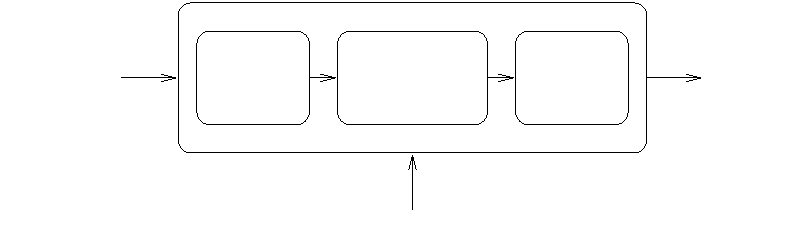
\includegraphics{hiq-arch.ps}
\else
  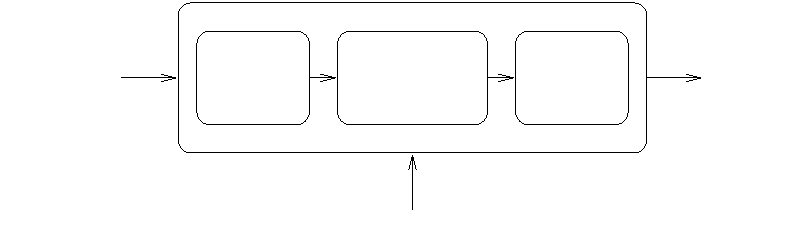
\includegraphics{hiq-arch.pdf}
\fi
\end{picture}
\setlength{\unitlength}{3947sp}%
%
\begingroup\makeatletter\ifx\SetFigFont\undefined%
\gdef\SetFigFont#1#2#3#4#5{%
  \reset@font\fontsize{#1}{#2pt}%
  \fontfamily{#3}\fontseries{#4}\fontshape{#5}%
  \selectfont}%
\fi\endgroup%
\begin{picture}(6374,1941)(376,-1315)
\put(6151,-61){\makebox(0,0)[lb]{\smash{{\SetFigFont{12}{14.4}{\familydefault}{\mddefault}{\updefault}{Results}%
}}}}
\put(376,-61){\makebox(0,0)[lb]{\smash{{\SetFigFont{12}{14.4}{\familydefault}{\mddefault}{\updefault}{Input deck}%
}}}}
\put(2701,-1261){\makebox(0,0)[lb]{\smash{{\SetFigFont{12}{14.4}{\familydefault}{\mddefault}{\updefault}{Programmatic user interface}%
}}}}
\put(2026,-61){\makebox(0,0)[lb]{\smash{{\SetFigFont{12}{14.4}{\familydefault}{\mddefault}{\updefault}{Models}%
}}}}
\put(3151,-61){\makebox(0,0)[lb]{\smash{{\SetFigFont{12}{14.4}{\familydefault}{\mddefault}{\updefault}{Assembly}%
}}}}
\put(4576,-61){\makebox(0,0)[lb]{\smash{{\SetFigFont{12}{14.4}{\familydefault}{\mddefault}{\updefault}{Solvers}%
}}}}
\end{picture}%
 }
  \end{center}
  \caption{Architecture of \hiq}
\end{figure}

The main components of \hiq\ are as follows.

\begin{itemize}
\item The mesh description language

The main way to describe devices in \hiq\ is to write a mesh input
deck using the Lua programming language (\ttt{http://www.lua.org}).
Because meshes are generated programmatically, it is easy to create
parameterized descriptions with hierarchies and arrays.

\item The programmatic user interfaces

There are two versions of the user interface: the MATLAB interface and
the standalone interface.  When using the MATLAB interface, a user has
access to the full range of MATLAB's numerical solvers and graphics
routines.  When using the standalone interface, a user does not have
as many built-in capabilities; but because the standalone interface
does not rely on MATLAB, it takes less memory and can solve larger
problems.  Like the mesh description interface, the user interface is
written in the Lua language, and is fully programmable.  We describe
both the MATLAB interface and the standalone interface in this manual.

\item The element model library

The element library includes linear, quadratic, and cubic quad and
brick elements for elastic problems and coupled thermoelastic problems
in plane strain, plane stress, axisymmetry, or three dimensions.  The
code also provides scalar wave equation elements in one, two, or three
dimensions.  For both scalar and elastic waves, the code supports
\emph{perfectly matched layer} sbsorbing boundaries to mimic the
effect of infinite domains.

\item The solver library

The solver library includes code for
\begin{itemize}
  \item Modal analysis of structures with anchor loss and
    thermoelastic damping.
  \item Forced response analysis, including forced response
    visualization and Bode plot construction.  The forced response
    analysis routines incorporate reduced order models.
\end{itemize}

\end{itemize}


\subsection{Download and basic setup}

The fastest way to get started with \hiq\ is to use the pre-compiled
version, available for Linux or Windows machines.  You can download
the source code and pre-compiled executables at
\begin{verbatim}
   http://www.cs.berkeley.edu/~dbindel/hiqlab/
\end{verbatim}
If you wish to run \hiq\ with the MATLAB interface, you will need
MATLAB version 6 or later.

If you wish to build your own version of \hiq, you will need
\begin{itemize}
  \item A C/C++ compiler and a FORTRAN 77 compiler (we have used the
    GNU compiler on Linux and Windows, and the Intel compilers on
    Itanium)
  \item Perl 5.002 or later
  \item LAPACK and BLAS (Basic Linear Algebra Subroutine) libraries.
    If you are compiling the MATLAB front-end for \hiq, these are
    already provided.
  \item UMFPACK (a linear system solver)
  \item ARPACK (an iterative eigenvalue solver)
\end{itemize}
If these packages are installed, you should be able to configure and
compile the software by running the following commands from the \hiq\
top-level directory:
\begin{verbatim}
  ./configure
  make
\end{verbatim}

At the time this manual is being written, \hiq\ is \emph{alpha}
software.  The code is still changing rapidly, and if you have trouble
setting up the program and running basic examples, please check to
make sure you have the most recent version.


\subsubsection{Running in MATLAB}

Once you have downloaded the pre-compiled version of the code (or once
you have built your own version), start MATLAB and run the file
\ttt{init.m}.  You should see something like the following:
\begin{verbatim}
 
                              < M A T L A B >
                  Copyright 1984-2001 The MathWorks, Inc.
                       Version 6.1.0.450 Release 12.1
                                May 18 2001
 
  
  To get started, type one of these: helpwin, helpdesk, or demo.
  For product information, visit www.mathworks.com.
  
>> init
HiQlab 0.2
Copyright   : Regents of the University of California
Build system: i686-pc-linux-gnu
Build date  : Tue Mar  1 12:51:22 PST 2005
Bug reports : dbindel@cs.berkeley.edu
>>
\end{verbatim}

\emph{You must run \ttt{init} before using \hiq from MATLAB.}  The
\ttt{init} script sets the MATLAB path variable so that MATLAB can
find the files \hiq\ needs for its analyses.

If you run \ttt{init} and see the \hiq\ banner, that means that you
have a working version of the MATLAB \hiq\ interface for your
machine.  If there is an error message when you run \ttt{init},
please send an e-mail including the exact error message, operating
system version, and MATLAB version.


\subsubsection{Running in standalone mode}

If you want to use the standalone version, look for an executable file
called \ttt{hiqlab} in the \ttt{src/lua} subdirectory.  When you
run \ttt{hiqlab} with no arguments, you should see an banner with
program information and a control prompt:
\begin{verbatim}
[dbindel@localhost lua]$ ./hiqlab
-------------------------------------------------------
HiQlab 0.2
Copyright   : Regents of the University of California
Build system: i686-pc-linux-gnu
Build date  : Thu Mar  3 19:29:03 PST 2005
Bug reports : dbindel@cs.berkeley.edu
 
Lua 5.0.2  Copyright (C) 1994-2004 Tecgraf, PUC-Rio
-------------------------------------------------------
 
>
\end{verbatim}%$
To end the \hiq\ session, press Ctrl-D on the keyboard.  \hiq\ may
also be run non-interactively: if \ttt{batch.lua} is a script that
runs an analysis and prints it out, for example, you might run
\begin{verbatim}
hiqlab batch.lua
\end{verbatim}

Like the MATLAB interface, the standalone user interface needs to know
where to find files.  The \ttt{init.lua} file in the \hiq\ main
directory specifies these files.  The first line of \ttt{init.lua}
has the form
\begin{verbatim}
HOME='/my/hiq/directory'
\end{verbatim}
where ``my hiq directory'' should be replaced by the directory
where \hiq\ is installed.  This is usually done automatically at
configuration time.  You can ensure that \hiq\ executes
\ttt{init.lua} when it starts in one of two ways:
\begin{enumerate}
\item Set the \ttt{HIQ\_INIT} environment variable to point to the
  full path for \ttt{init.lua}.  \hiq\ calls any files specified in
  the \hiq\ directory
\item Specify \ttt{init.lua} using the \ttt{-l} argument to
  \hiq.  For example, to execute \ttt{init.lua} before running
  \hiq\ in interactive mode,
\begin{verbatim}
hiqlab -l /my/hiq/directory/init.lua -i
\end{verbatim}
  and to run a batch script,
\begin{verbatim}
hiqlab -l /my/hiq/directory/init.lua batch.lua
\end{verbatim}
\end{enumerate}


\subsection{``Hello world'' in \hiq}

\subsubsection{Describing a cantilever beam}

\begin{figure}
\begin{verbatim}
require 'common.lua'
 
l = 10e-6         -- Beam length
w = 2e-6          -- Beam width
dense = 0.5e-6    -- Approximate element size (for block generator)
order = 2         -- Order of elements
 
mesh  = Mesh:new(2)
mat   = make_material('silicon2', 'planestrain')
mesh:blocks2d( { 0, l }, { -w/2.0, w/2.0 }, mat )
 
mesh:set_bc(function(x,y)
  if x == 0 then return 'uu', 0, 0; end
end)
\end{verbatim}
\caption{The complete mesh input file for a cantilever beam}
\label{mesh-input-fig}
\end{figure}

Figure~\ref{mesh-input-fig} shows the input file used to describe a
simple cantilever beam.  We now describe the input file in detail.  

\begin{itemize}

\item Including common support files:
\begin{verbatim}
require 'common.lua'
\end{verbatim}

Typically, input files will start with one or more \ttt{require}
statements, which are used to load function definitions, material
databases, and other data.  The \ttt{require} statement is much
like an include statement in C or Fortran, except that
\ttt{require} loads each file \emph{once}.  For example, the file
\ttt{common.lua} begins by requiring \ttt{material.lua}; if my
input file also started with a line \ttt{require 'material.lua'},
I would not end up with two copies of the material definitions file.

When the interpreter encounters a \ttt{require} statement, it
searches through a standard path to find a file with a matching name.
We will say more about the search path in
Section~\ref{require-section}.  The file \ttt{common.lua}, which is
defined in \ttt{models/common.lua} provides functions that are
useful for defining element types; \ttt{common.lua} should be
included in most mesh description files.

\item Defining geometric parameters:
\begin{verbatim}
l = 10e-6         -- Beam length
w = 2e-6          -- Beam width
\end{verbatim}

A two-dimensional beam model must have a length and a width.  These
two lines give the beam length (10 \mum) and width (2 \mum) in MKS
units.  Giving names to geometric parameters makes the input file
easier to read than it would otherwise be.  In
Section~\ref{parameterization-section}, we describe how named
parameters can be set from outside the input file in order to simplify
parameter studies.

\item Defining mesh generation parameters:
\begin{verbatim}
dense = 0.5e-6    -- Approximate element size (for block generator)
order = 2         -- Order of elements
\end{verbatim}

The mesh file must describe both the geometry of the device and the
parameters that define the mesh.  \hiq\ includes several functions
that define regular ``blocks'' that can be tied together to form a
mesh.  The \texttt{dense} and \texttt{order} parameters control how
\hiq\ builds these blocks.  The \texttt{order} parameter is the order
of polynomial interpolation used within each element: linear,
quadratic, and cubic elements are available.  The \texttt{dense}
parameter describes the element size.

\item Creating a mesh object:
\begin{verbatim}
mesh = Mesh:new(2)
\end{verbatim}

All information about the mesh is stored in a mesh object.  The mesh
constructor has a single argument, the dimension of the ambient space
for the problem.  The mesh object should be called \ttt{mesh}.

\item Defining a material:
\begin{verbatim}
mat = make_material('silicon2', 'planestrain')
\end{verbatim}

Build an element type for computing the response of silicon in plane
strain.  The first argument refers to an entry in \ttt{materials.lua}
which defines material arguments like Young's modulus and the Poission
ratio; subsequent arguments define the type of analysis (plane stress,
plane strain, axisymmetric, or three-dimensional).


\item Defining the mesh:
\begin{verbatim}
mesh:blocks2d( { 0, l }, { -w/2.0, w/2.0 }, mat )
\end{verbatim}

The mesh for a cantilever beam is simple: it covers the rectangular
region $[0,l] \times [-w/2,w/2]$.  The \ttt{blocks2d} generator
creates such a region and adds it to the mesh; the element size and
order are determined by the global variables \ttt{dense} and
\ttt{order} defined earlier, and the \ttt{mat} parameter from the
previous line defines which material should be used.


\item Defining boundary conditions:
\begin{verbatim}
mesh:set_bc(function(x,y)
  if x == 0 then return 'uu', 0, 0; end
end)
\end{verbatim}

By calling \ttt{mesh:set\_bc(myfunc)}, we define boundary conditions
for the problem.  \ttt{myfunc} may be an anonymous function (a
function without an explicitly assigned name), which is what we use
for this problem.  The function is called at every node in the mesh.
If the call returns nothing, then no boundary conditions are applied;
otherwise, the call returns a string which defines whether essential
or natural (displacement or flux) boundary conditions are applied.  In
this example, displacement boundary conditions (denoted by 'u') are
given for both the $x$ and $y$ displacements.  The two numeric
arguments after the string indicate that the $x$ and $y$ displacements
are set to zero.

\end{itemize}

\subsubsection{Eigenvalue analysis in MATLAB}
\subsubsection{Eigenvalue analysis in standalone mode}

\subsection{Getting help}

\newpage
\section{Basic features from Lua}
\emph{Write about and or features!!}

\subsection{Variable types}
Since Lua is a dynamically typed language, there
are no type definitions in the language. In other
words, the type is defined by the variable assigned. 
There are eight basic types in Lua. Of these the
{\tt HiQLab} user should be aware of the following 6.
\begin{enumerate}
\item {\tt nil}: This is the type that is assigned to all variables
by default. {\tt nil} can be assigned to a variable as,
\begin{verbatim}
   a = nil
\end{verbatim}
\item {\tt boolean}: This has two types, {\tt true}and {\tt false}. 
In Lua, any value may represent a condition. In conditionals,
\emph{ONLY} {\tt false} and {\tt nil} are considered false, and everything
else is considered true. Beware that the value zero and empty string
both represent \emph{TRUE}. 
\item {\tt number}: Lua has only one number type, real double-precision
floating point numbers. There are \emph{NO} integer types. Valid types
of number representations are,
\begin{verbatim}
            4     0.4    4.57e-3   0.3e12   5e+20
\end{verbatim}
\item {\tt string}: Strings have the usual meaning, a sequence of 
characters. The string can be assigned by putting them between 
single quotes or double quotes. They can be assigned to a variable 
by the following statement.
\begin{verbatim}
   a = "a line"
   b = 'another line'
\end{verbatim}
Strings in Lua can contain the following C-like escape sequences:
\begin{table}[htbp]
\caption{C-like escape sequences}
\centering
\begin{tabular}{c|c}
{\tt \textbackslash b} & : back space \\
{\tt \textbackslash n} & : newline \\
{\tt \textbackslash t} & : horizontal tab \\
{\tt \textbackslash v} & : vertical tab \\
{\tt \textbackslash\textbackslash} & : back slash \\
{\tt \textbackslash '} & : single quote \\
{\tt \textbackslash "} & : double quote 
\end{tabular}
\end{table}

Strings can be concatenated by the operator {\tt ..}.
\begin{verbatim}
   a = "Hello"
   b = "World"
   c = a..b
   d = a.." "..b
   print(c)         --> HelloWorld
   print(d)         --> Hello World
\end{verbatim}

\item {\tt table}: This type is used to implement associative arrays.
An associative array is an array that can be indexed not only with
numbers, but also with strings or any other value of the language. 
Moreover, tables have no fixed size, and the size is adjusted dynamically.
Thus a single Lua table can contain different types of data.
\begin{verbatim}
   a    = {}               -- create a table
   a[1] = 4                -- store double
   a[21]= 'Hello world'    -- store string
   print(a[1])             --> 4

   a['A']    = a           -- Index with character
   a['John'] = Doe         -- Index with string
   print(a['John'])        --> Doe
   print(a[John])          --> nil
\end{verbatim}
Tables in Lua are treated as objects similar to Java. Thus a
program that manipulates tables, only manipulates references
or pointer to them. 
\begin{verbatim}
   b =  a                  -- the reference to the table that 'a'
                          -- points to is passed
\end{verbatim}

Additionally, since tables are like objects,
{\tt a.name} cna be used as syntactic sugar for {\tt a["name"]}.
\begin{verbatim}
   a      = {}
   a["x"] = 4 
   print(a["x"])           --> 4
   print(a.x)              --> 4
\end{verbatim}
Tables can be initialied with values by the following argument,
in which case the keys to the corresponding values start from
one (and not with zero, as in C).
\begin{verbatim}
   a      = { 10, 11, 12}
   print(a[1])             --> 10
\end{verbatim}

\item {\tt function} This aspect will further be explained in
section ????.

\end{enumerate}

WHAT YOU SHOULD KNOW(Zentei Chishiki).

\subsection{Ending a line}
A statement in Lua is called a {\tt chunk},
and is simply a sequence of statements. 
This {\tt chunk} can take a single line,
multiple lines, or can even span multiple files.
A semicolon may optionally follow any statement,
but this is just a convention. Thus, the following
four chunks are equivalent.
\begin{verbatim}
   -- Chunk 1
   a = 1
   b = a*2

   -- Chunk 2
   a = 1;
   b = a*2

   -- Chunk 3
   a = 1; b = a*2

   -- Chunk 4
   a = 1  b = a*2
\end{verbatim}


\subsection{Print statement}
All variable types can be printed to the screen through
the command {\tt print}
\begin{verbatim}
   a = 4
   print(a)     --> 4
   b = "Hello World"
   print(b)     --> Hello World
   c = false
   print(c)     --> false
   d = {4, 5, 6}
   print(d)     --> table: 0x8067d90
                 (The reference is printed in this case)
   print(d[2])  --> 5
\end{verbatim}


\subsection{Comments}
A comment starts anywhere with a double hyphen (--)
and runs until the end of the line. Lua also offers
block comments, starting with {\tt --[[} and run till
{\tt --]]}.
\begin{verbatim}
   -- This is a commented line

   --[[
      print(10)             --This is a commented block
   --]]
\end{verbatim}

\subsection{For loops}
\ttt{for} loops in Lua are stated by the following 
structure.
\begin{verbatim}
   for var=start_value, end_value, increment do
       do something
   end
\end{verbatim}
The loop will execute \ttt{something} for each value
of \ttt{var} from \ttt{start\_value} to \ttt{end\_value}
with and increment of \ttt{increment}. If \ttt{increment}
is absent, the increment will be assumed one. 

An example for printing the numbers 1 through 10 is 
presented below.  
\begin{verbatim}
for i=1,10 do
  print(i)  
end
\end{verbatim}
One remark that should be made is that in the example
above the index $i$ is declared as a local variable.
This implies that once the for loop is terminated the
value of $i$ will not be retained and cannnot be referenced
to.

\subsection{If statements}
\ttt{if} statements in Lua are defined by the following 
structures.
\begin{verbatim}
   if condition_expression then
      do something
   end
\end{verbatim}
or,
\begin{verbatim}
   if condition_expression then
      do something
   else
      do something else
   end
\end{verbatim}
All other values other than \ttt{false} or \ttt{nil} that
are returned by the \ttt{condition\_expression} will be 
treated as \ttt{true}.

An example code to print the larger of the value \ttt{a,b}
is:
\begin{verbatim}
   if a > b then
      print(a)
   else
      print(b)
   end
\end{verbatim}

To avoid writing nested \ttt{if}s, one can use
\ttt{elseif} in the following structure.
\begin{verbatim}
   if condition_expression then
      do something
   elseif condition_expression
      do something else
   else
      do yet something else
   end
\end{verbatim}

\subsection{Functions}
A function in Lua is defined by the following 
format.
\begin{verbatim}
   function function_name(input_arguments)
      function_body
   end
\end{verbatim}

The input arguments can any type of Lua variable,
and when multiple values are passed, they must be 
seperated by a comma. It is possible to assign
no input arguments.

\ttt{function\_body} will consist of the standard
Lua chunks. For the function to return an output 
value the \ttt{return} command must be placed.
\begin{verbatim}
   function function_name(input_arguments)
      function_body
      return output_arguments
   end
\end{verbatim}
\ttt{output\_arguments} may return any type of Lua
variable, and when multiple values are returned, they
must be seperated by a comma.

An example of a function which takes two numbers \ttt{a,b}
as the input and returns their sum is 
shown below.
\begin{verbatim}
   function add(a,b)

      sum_ab = a + b

      return sum_ab
   end
\end{verbatim} 
The method of calling this function is the following.
\begin{verbatim}
   a = 4
   b =-2.11
   sum_ab = add(a,b)
   print(sum_ab)      -> 1.89
\end{verbatim}
The function above can be modified to also return the difference
by the following code.
\begin{verbatim}
   function add_diff(a,b)

      sum_ab = a + b
      diff_ab= a - b

      return sum_ab, diff_ab
   end
\end{verbatim} 
The method of calling this function is the following.
\begin{verbatim}
   a = 4
   b =-2.11
   sum_ab, diff_ab = add_diff(a,b)
   print(sum_ab)      -> 1.89
   print(diff_ab)     -> 6.11
\end{verbatim}


\newpage
\section{Mesh description (Lua)}
\subsection{\ttt{require} statements and common files}
\label{require-section}
\emph{Need directory tree diagram or something}

Typically, mesh input files will start with one or more \ttt{require}
statements, which are used to load function definitions, material
databases, and other data.  The \ttt{require} statement is much
like an include statement in C or Fortran, except that
\ttt{require} loads each file \emph{once}.  For example, the file
\ttt{common.lua} begins by requiring \ttt{material.lua}; if my
input file also started with a line \ttt{require 'material.lua'},
I would not end up with two copies of the material definitions file.
When the interpreter encounters this \ttt{require} statement, it
searches through a standard path to find a file with a matching name.

The file \ttt{common.lua}, which is
defined in \ttt{models/common.lua} provides functions that are
useful for defining element types; \ttt{common.lua} should be
included in most mesh description files. The 
functions contained in \ttt{common.lua} are sorted by functionality
and presented in table \ref{table:FunctionsInCommonDotLua}. Further
details on the input and output arguments of the function are 
given in the section?? related with non-dimensionalization and 
section??? related with material models.

The file \ttt{material.lua}, which is
defined in \ttt{models/material.lua} provides a material database
which is useful for defining element types; \ttt{materials.lua} is
automatically incorporated by including the file \ttt{common.lua}. The 
functions contained in \ttt{materials.lua} are sorted by functionality
and presented in table \ref{table:FunctionsInMaterialsDotLua}. 
The materials in the database are sorted by the type of analysis they
are capable of in table \ref{table:MaterialsInMaterialsDotLua}.
Further details on the input and output arguments of the functions and
properties of the materials are 
given in the section?? related with material models.

\begin{table}[htbp]
\caption{Functions contained in \ttt{common.lua}}
\label{table:FunctionsInCommonDotLua}
\vspace{0.1in}
\centering
\begin{tabular}{m{2in}|m{3in}}
\hline
\multicolumn{1}{c|}{\tbf{Functionality}} & 
\multicolumn{1}{c}{\tbf{Function name}} \\
\hline
\hline
Retrieve material property values &
\ttt{get\_material(mtype)} \\
\hline
Set characteristic scales for non-dimensionalization &
\ttt{mech\_nondim(mtype,cL)},
\ttt{ted\_nondim(mtype,cL)},
\ttt{pz\_nondim(mtype,cL)},
\ttt{em\_nondim(mtype,cL,eps)} \\
\hline
Non-dimensionlize material properties &
\ttt{mech\_material\_normalize(mtype)},
\ttt{ted\_material\_normalize(mtype)},
\ttt{pz\_material\_normalize(mtype)} \\
\hline
Construct element with \ttt{mtype} material property &
\ttt{make\_material(mtype,etype,wafer,angle)},
\ttt{make\_material\_te(mtype,etype,wafer,angle)},
\ttt{make\_material\_pz(mtype,etype,wafer,angle)},
\ttt{make\_material\_couple\_em2d(eps,etype)}\\
\hline
\end{tabular}
\end{table}

\begin{table}[htbp]
\caption{Functions contained in \ttt{materials.lua}}
\label{table:FunctionsInMaterialsDotLua}
\vspace{0.1in}
\centering
\begin{tabular}{m{2in}|m{2in}}
\hline
\multicolumn{1}{c|}{\tbf{Functionality}} & 
\multicolumn{1}{c}{\tbf{Function name}} \\
\hline
\hline
Assign proper mechanical variables if non-existent&
\ttt{fill\_mech(mtype)} \\
\hline
Assign proper piezoelectric variables if non-existent &
\ttt{fill\_piezo(mtype)} \\
\hline
\end{tabular}
\end{table}

\begin{table}[htbp]
\caption{Materials contained in \ttt{materials.lua}}
\label{table:MaterialsInMaterialsDotLua}
\vspace{0.1in}
\centering
\begin{tabular}{l|c|c|c|c|c}
\hline
\multicolumn{1}{c|}{\tbf{Material name}} &
\multicolumn{1}{c|}{\tbf{Crystal}}       &
\multicolumn{4}{c}{\tbf{Analysis}} \\
\cline{3-6}
  &  &  \ttt{mech}  & \ttt{thermoelastic} 
     &  \ttt{piezo} & \ttt{electromech} \\
\hline
\hline
\ttt{sc\_silicon}   & cubic 
& $\bigcirc$ & $\bigcirc$ & $\times$ & $\bigcirc$ \\
\ttt{poly\_silicon} & isotropic 
& $\bigcirc$ & $\bigcirc$ & $\times$ & $\bigcirc$ \\
\ttt{amor\_silicon} & cubic
& $\bigcirc$ & $\bigcirc$ & $\times$ & $\bigcirc$ \\
\ttt{silicon} & isotropic
& $\bigcirc$ & $\times$   & $\times$ & $\bigcirc$ \\
\ttt{silicon2} & isotropic 
& $\bigcirc$ & $\bigcirc$ & $\times$ & $\bigcirc$ \\
\hline
\ttt{hfo2}   & isotropic 
& $\bigcirc$ & $\times$   & $\times$ & $\bigcirc$ \\
\ttt{sic}    & isotropic 
& $\bigcirc$ & $\times$   & $\times$ & $\bigcirc$ \\
\ttt{sige}   & isotropic 
& $\bigcirc$ & $\times$   & $\times$ & $\bigcirc$ \\
\ttt{siox}   & isotropic 
& $\bigcirc$ & $\times$   & $\times$ & $\bigcirc$ \\
\ttt{diamond}& isotropic 
& $\bigcirc$ & $\times$   & $\times$ & $\bigcirc$ \\
\hline
\ttt{aln}    & hexagonal
& $\bigcirc$ & $\times$   & $\bigcirc$& $\times$ \\
\ttt{aln\_isotropic}    & isotropic
& $\bigcirc$ & $\times$   & $\bigcirc$& $\times$ \\
\ttt{aln\_piazza}    & hexagonal
& $\bigcirc$ & $\times$   & $\bigcirc$& $\times$ \\
\ttt{pt\_piazza}    & isotropic
& $\bigcirc$ & $\times$   & $\times$& $\bigcirc$ \\
\ttt{al\_piazza}    & isotropic
& $\bigcirc$ & $\times$   & $\times$& $\bigcirc$ \\
\hline
\end{tabular}
\end{table}

\clearpage
\subsection{Constructing the \tt{Mesh} object}

All the information about the mesh is stored in a 
mesh object. The mesh constructor has a single argument,
the dimension of the ambient space for the problem. 
\begin{codelist}
  \item{Mesh(ndm)} A mesh object with \ttt{ndm} dimensions
  for the ambient space. 
\end{codelist}
The mesh object should be called \ttt{mesh}. The mesh is
usually constructed by the following statement.
\begin{verbatim}
   mesh = Mesh:new(ndm)
\end{verbatim}

\subsection{Adding nodes}
Nodal points must be defined in order to construct the mesh.
There are two primitive operations to add nodes to the mesh geometry.
\begin{codelist}

  \item[add\_node(x)]
    Adds a single node with positions listed consecutively in the
    array \ttt{x=\{x1,y1\}}, and returns the identifier of the node.
  \item[add\_node(x,n)]
    Adds \ttt{n} nodes with positions listed consecutively in the
    array \ttt{x=\{x$_1$,$\ldots$,x$_{n}$\}}, and returns the 
    identifier of the first node.

\end{codelist}
It must be noted that the identifier of the nodes are 0 based in the
Lua environment. Thus the the identifier returned after adding the
very first node will be \emph{0}.

The nodes can be added to \ttt{mesh} by the following statements.
\begin{verbatim}
   x = {x1, y1,
        x2, y2,
        x3, y3}

   identifier_for_first_node = mesh:add_node(x,3)
\end{verbatim}

\subsection{Adding elements}
\subsubsection{Element types}
HiQLab currently supports line, quad, and brick elements for 
mechanical, thermomechanical, piezoelectric mechanical, and 
electromechanical problems. Details of implementation and
capabilities of each element are noted in section \ref{section:ElementLibrary},
which explains the element library.   

\subsubsection{Line, quad, and brick node ordering}
The current shape function library supports linear, quadratic, 
and cubic; and bilinear, biquadratic, and
bicubic quads; and trilinear, triquadratic, and tricubic bricks.  The
ordering is non-standard. For lines, the nodes are listed in
increasing order starting from one end node. This is shown in
Figure \ref{fig:NodeOrderingLine}.  

For quads, the nodes are listed in
increasing order by their coordinates, with the $y$ coordinate varying
fastest.  
For example, for 4-node,9-node, and 16-node quads, we use the
ordering shown in Figure~\ref{fig:NodeOrderingQuad}.  

The ordering in the
3D brick case is similar, but with the $z$ coordinate varying fastest, the
$y$ coordinate second-fastest, and the $x$ coordinate most slowly.
For example, for 8-node and 27-node bricks, we use the
ordering shown in Figure~\ref{fig:NodeOrderingBrick}.  

So long as the ordering in the spatial domain is consistent with the
ordering in the parent domain, the isoparametric mapping will be
well-behaved (so long as element distortion is not too great).  The
\ttt{add\_block} commands described in the section
\ref{section:BlockGenerators} produce node orderings which are
consistent with our convention.

The primary advantage of the node ordering we have chosen is that it
becomes trivial to write loops to construct 2D and 3D tensor product
shape functions out of simple 1D Lagrangian shape functions.  Also, it
becomes simple to write the loops used to convert a mesh of higher
order elements into four-node quads or eight-node bricks for
visualization (see Section~\ref{section-opendx}).

\devnote{Currently, the number of Gauss points used by the element
  library is fixed at compile time.  It might be wise to allow the
  user to change that.}

\subsubsection{Adding elements to mesh}
In order to add an element to the mesh, we must first 
construct an element object. This can be done by the
following statement.
\begin{verbatim}
   etype = mesh:Element(arguments)
\end{verbatim}
To construct a \ttt{PMLElastic2D} element, \ttt{Element}
is replaced by the following,
\begin{verbatim}
   etype = mesh:PMLElastic2d( E, nu, rho, analysis_type);
\end{verbatim}
Once this element object is constructed we must define the
connectivity of a particular element and add this to the
\ttt{mesh} object by the command:
\begin{codelist}

  \item[add\_element(con,etype,nen,num)]
    Adds \ttt{n} elements of type \ttt{etype} with node lists of
    length \ttt{nen} listed consecutively in the array \ttt{con},
    and returns the identifier of the first element added.

\end{codelist}
It must be noted that the identifier of the elements are 0 based in the
Lua environment. Thus the the identifier returned after adding the
very first element will be \emph{0}.

A sample code for adding one 4-noded quad element to the mesh 
would look like,
\begin{verbatim}
   con = { node_num1, node_num2, node_num3, node_num4}
   identifier_for_first_element = mesh:add_element(con, etype, 4, 1)
\end{verbatim}

\clearpage
\begin{figure}[htbp]
\centering
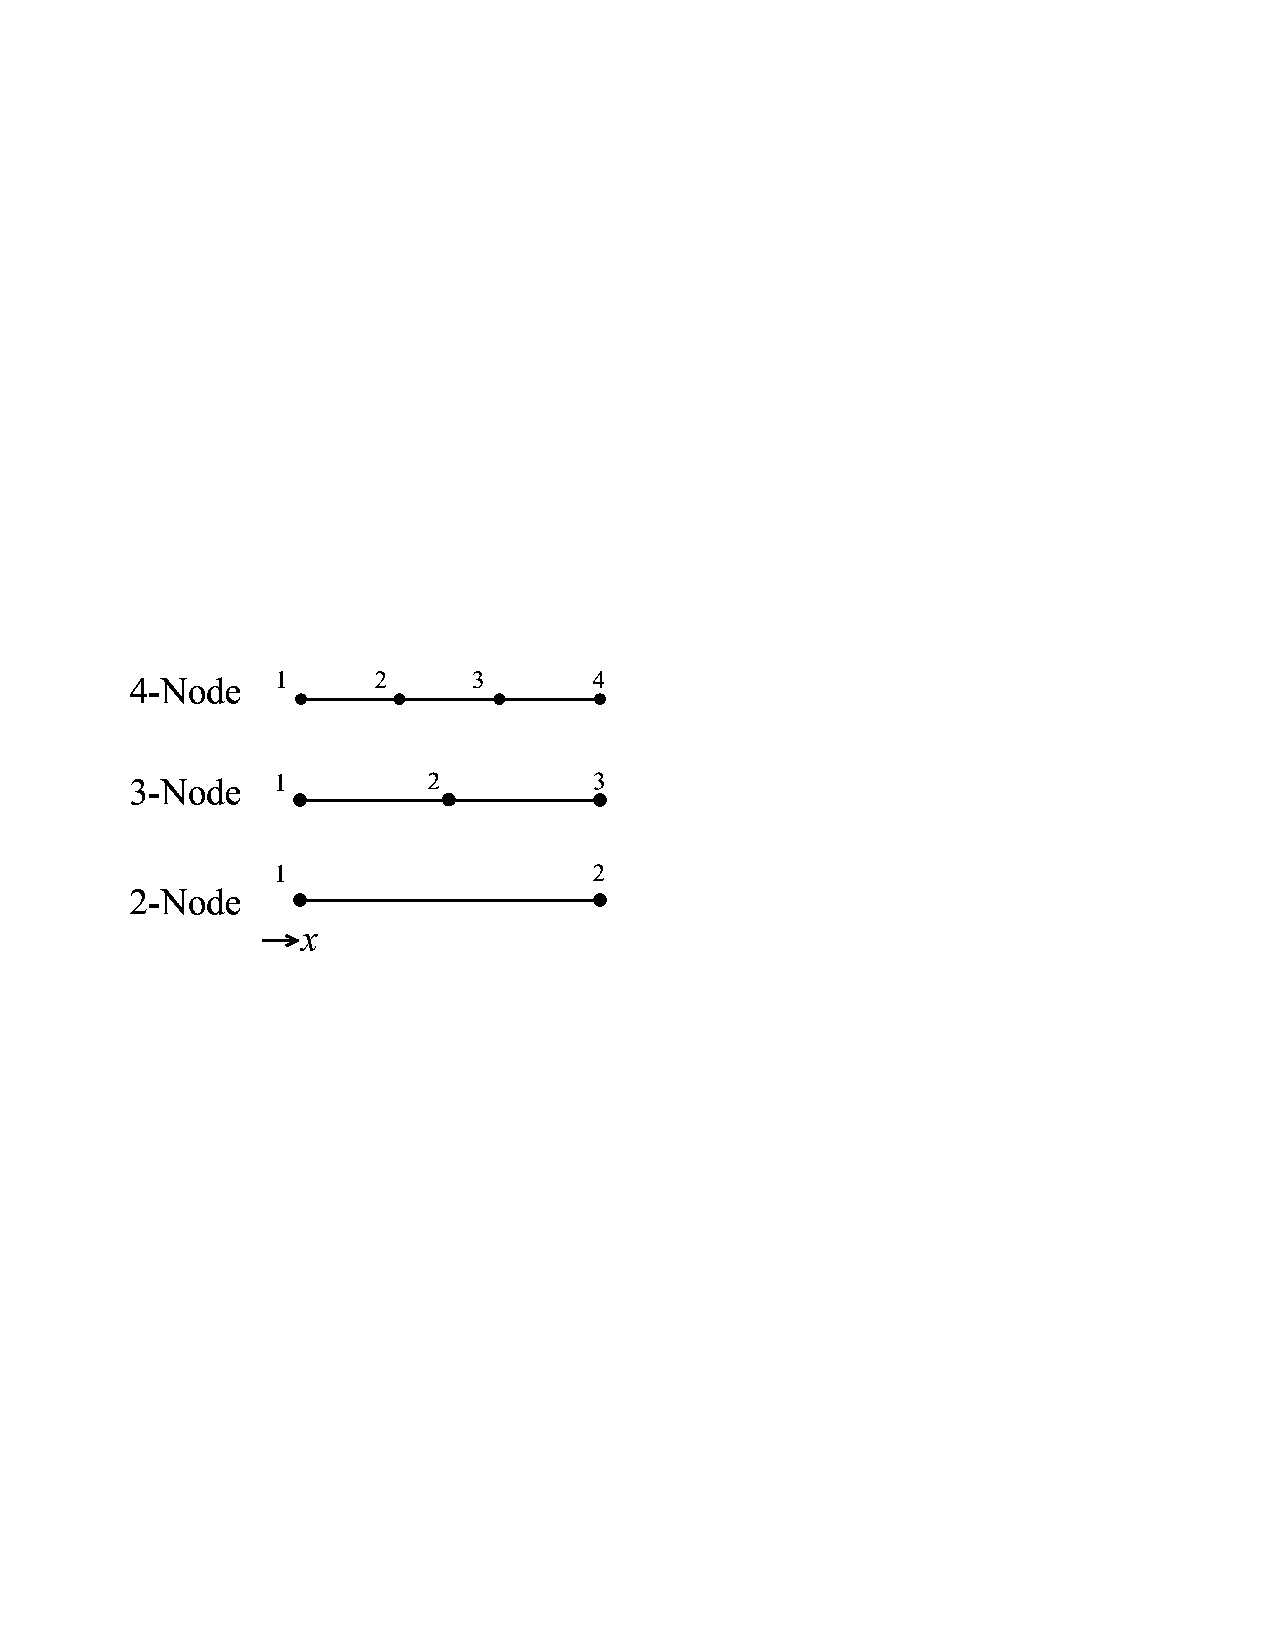
\includegraphics[trim=0.5in 4.5in 4.0in 4.0in, clip, height=1.6in]{fig/nodeordering1D.pdf}
\caption{Node ordering for 2-node, 3-node, and 4-node line elements}
\label{fig:NodeOrderingLine}
%\end{figure}
%\begin{figure}[htbp]
\begin{minipage}{\linewidth}
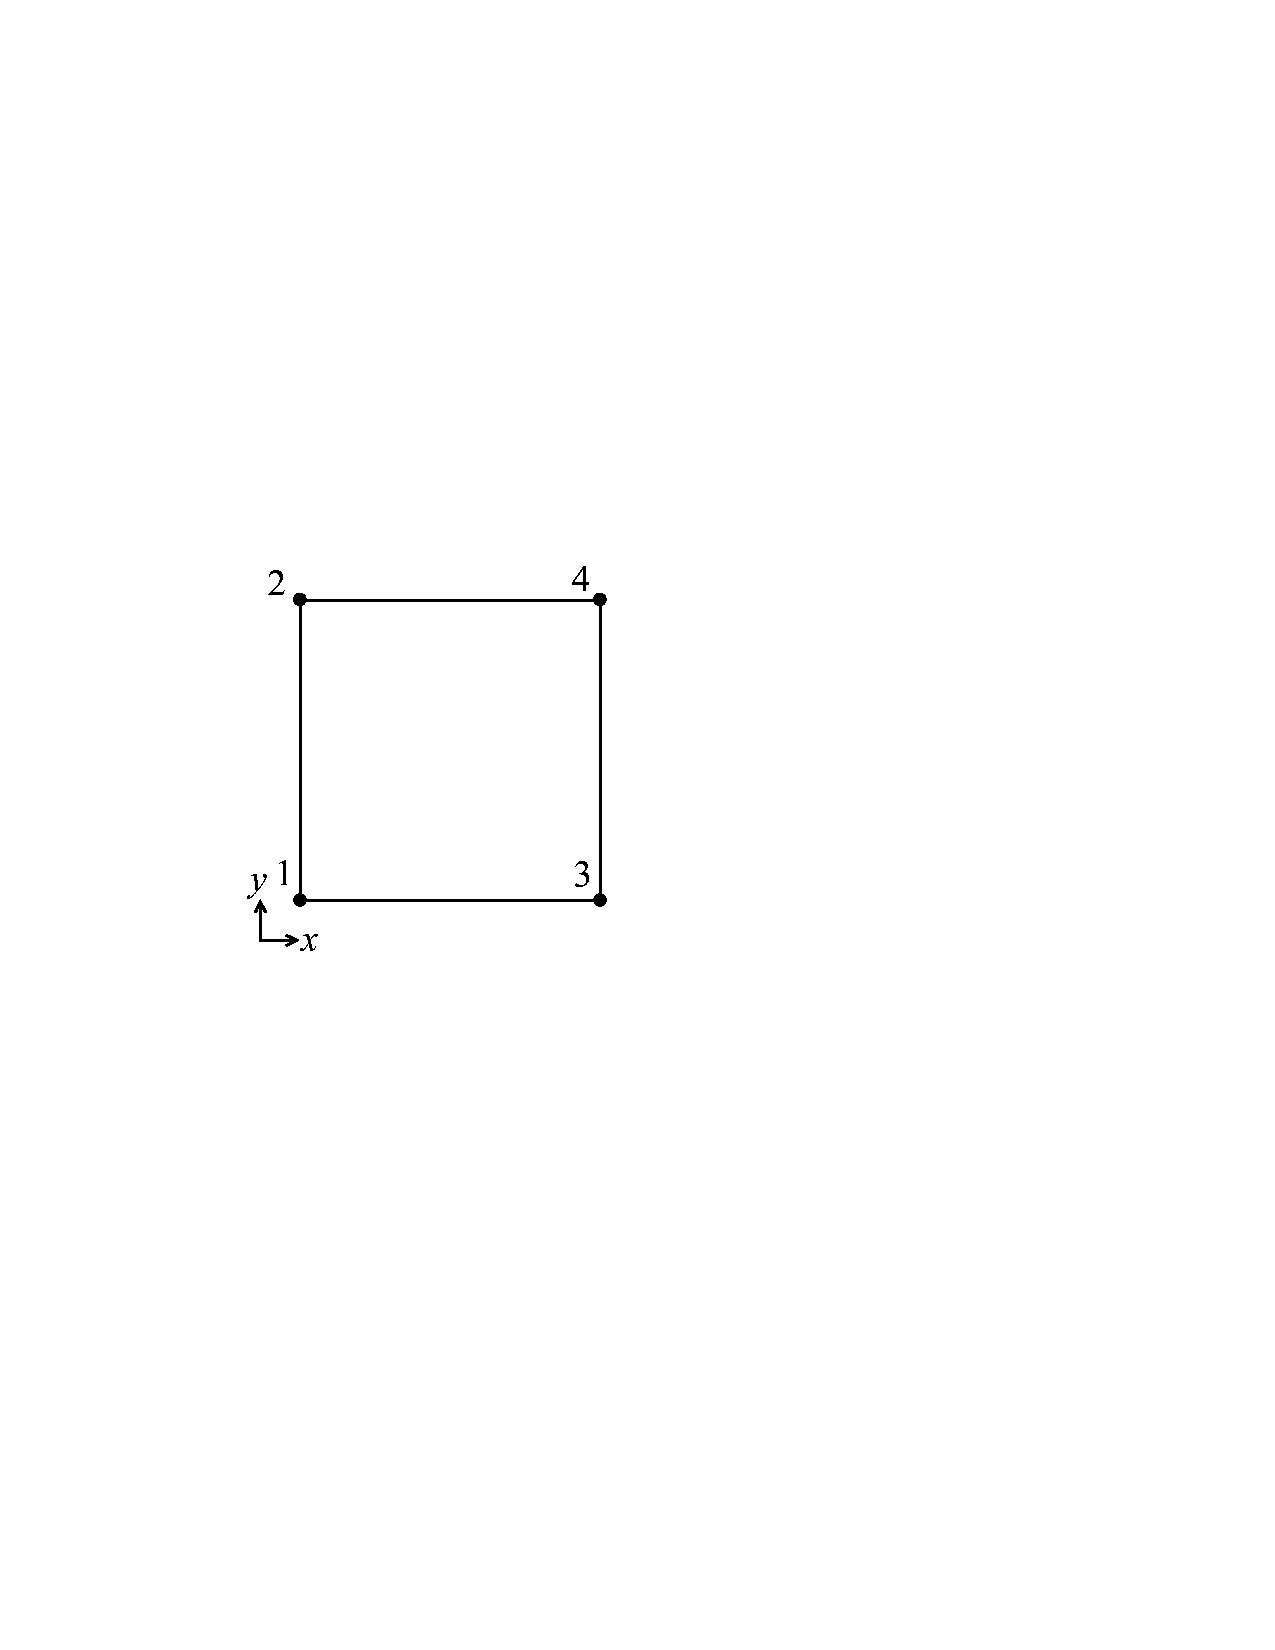
\includegraphics[trim=1.5in 4.5in 4.2in 3.5in, clip, height=2in]{fig/nodeordering2D_4.pdf}
\hfill
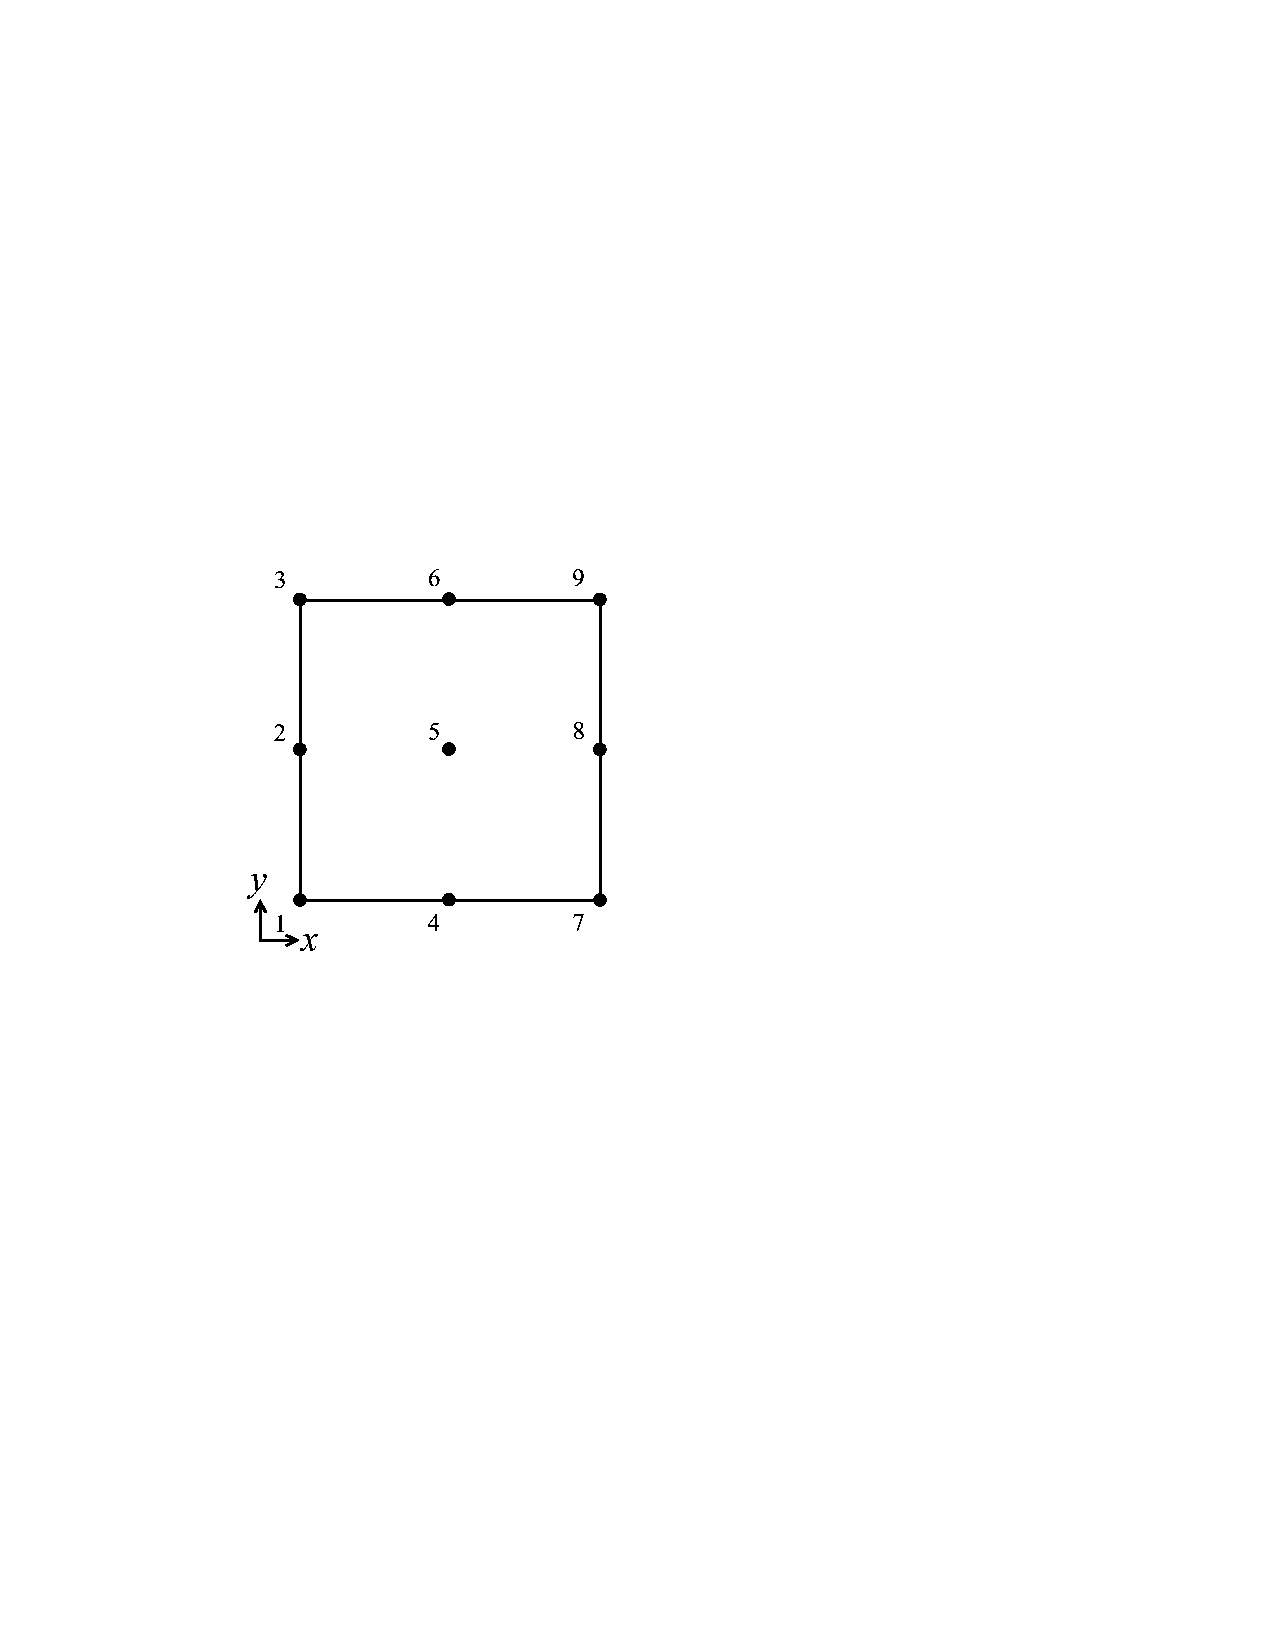
\includegraphics[trim=1.5in 4.5in 4.2in 3.5in, clip, height=2in]{fig/nodeordering2D_9.pdf}
\hfill
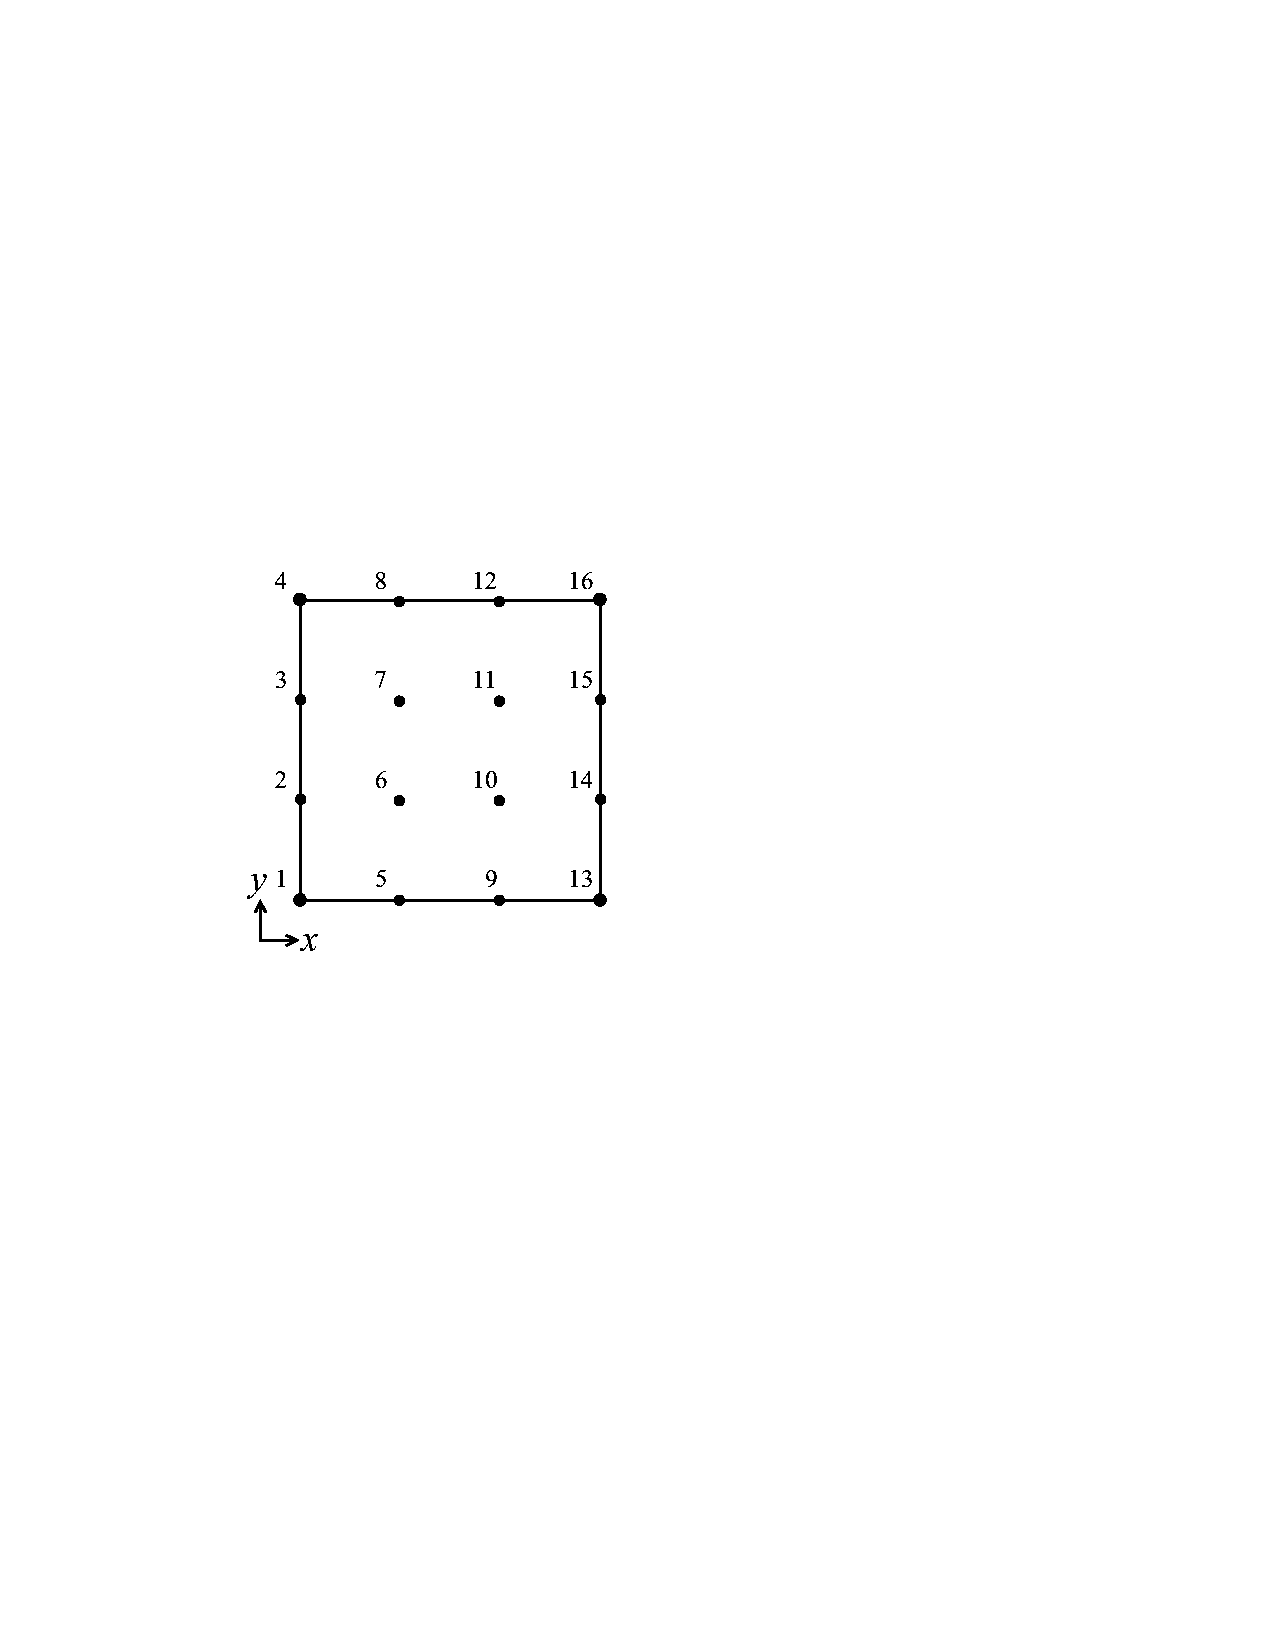
\includegraphics[trim=1.5in 4.5in 4.2in 3.5in, clip, height=2in]{fig/nodeordering2D_16.pdf}
\caption{Node ordering for 4-node, 9-node, and 16-node quads}
\label{fig:NodeOrderingQuad}
\end{minipage}
%\end{figure}
%\begin{figure}[htbp]
\centering
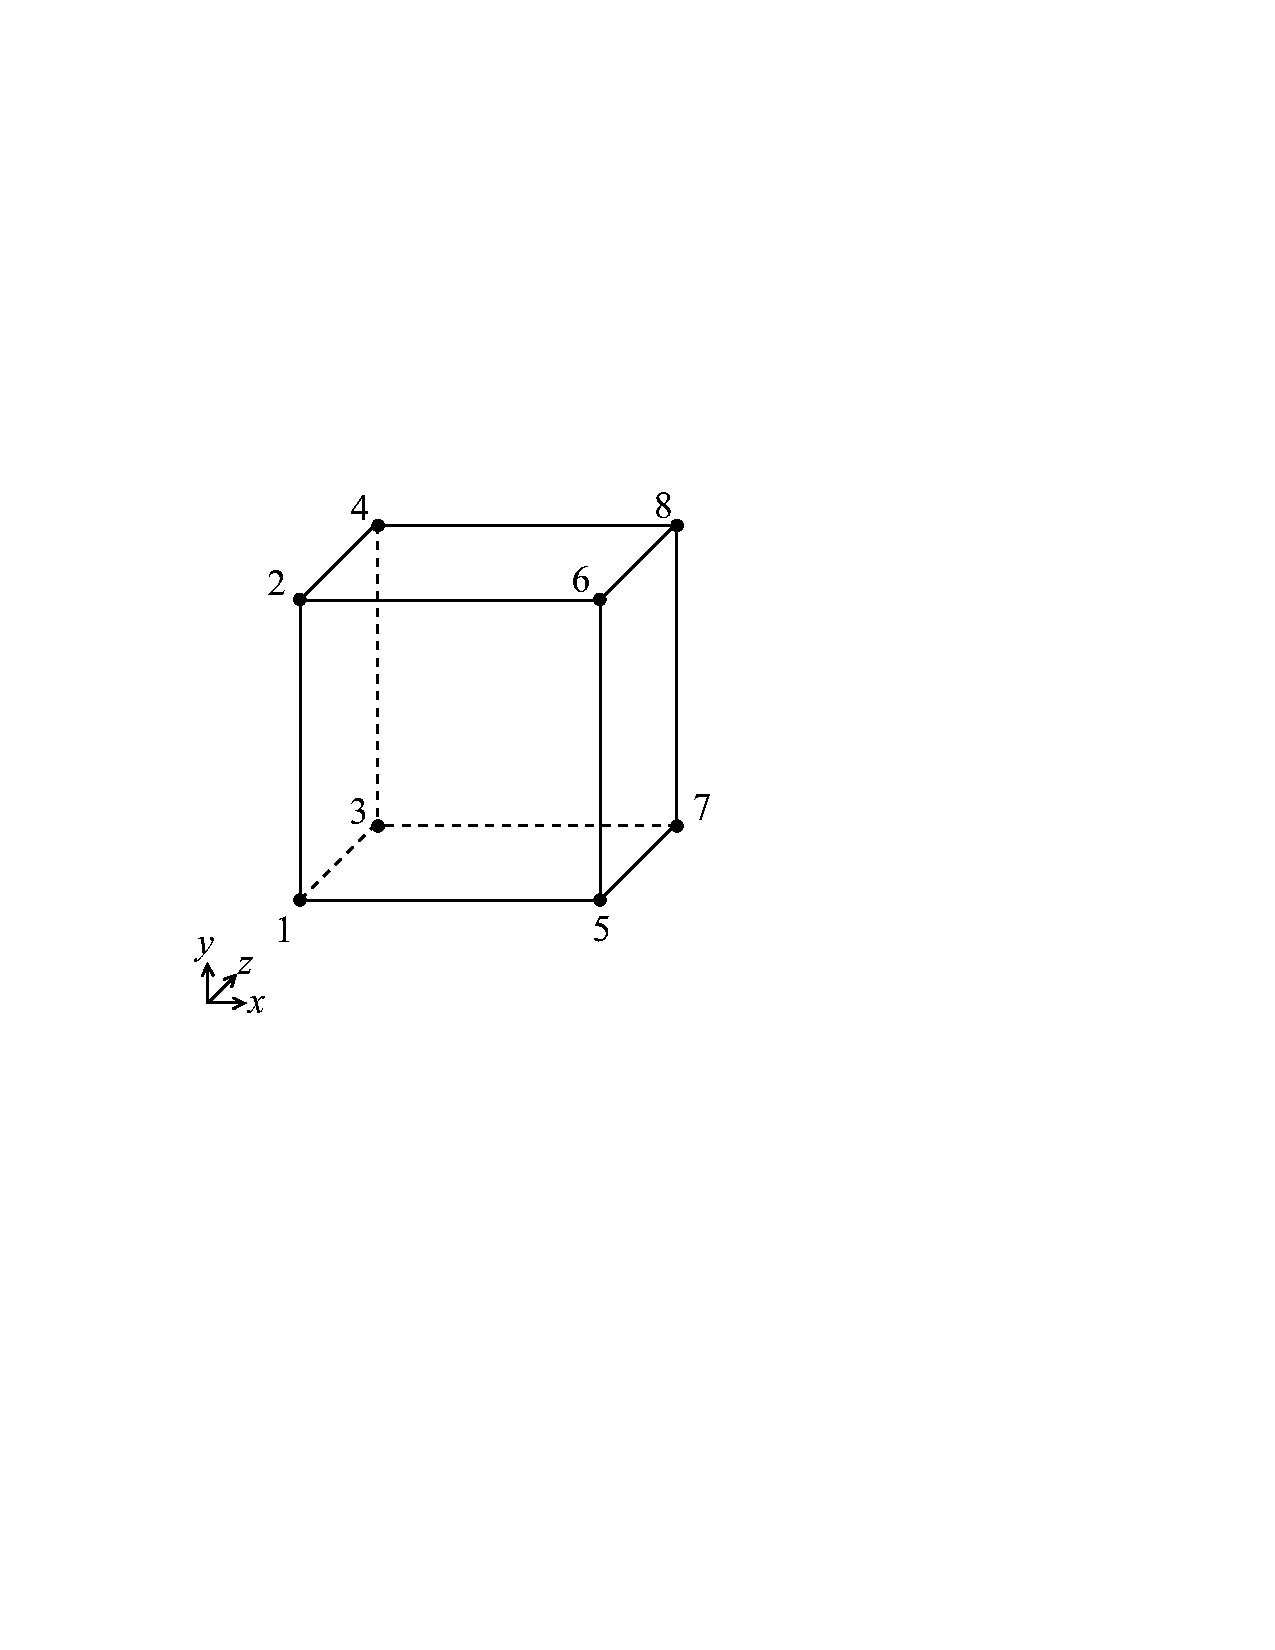
\includegraphics[trim=1.2in 4.2in 3.5in 3.0in, clip, height=2in]{fig/nodeordering3D_8.pdf}
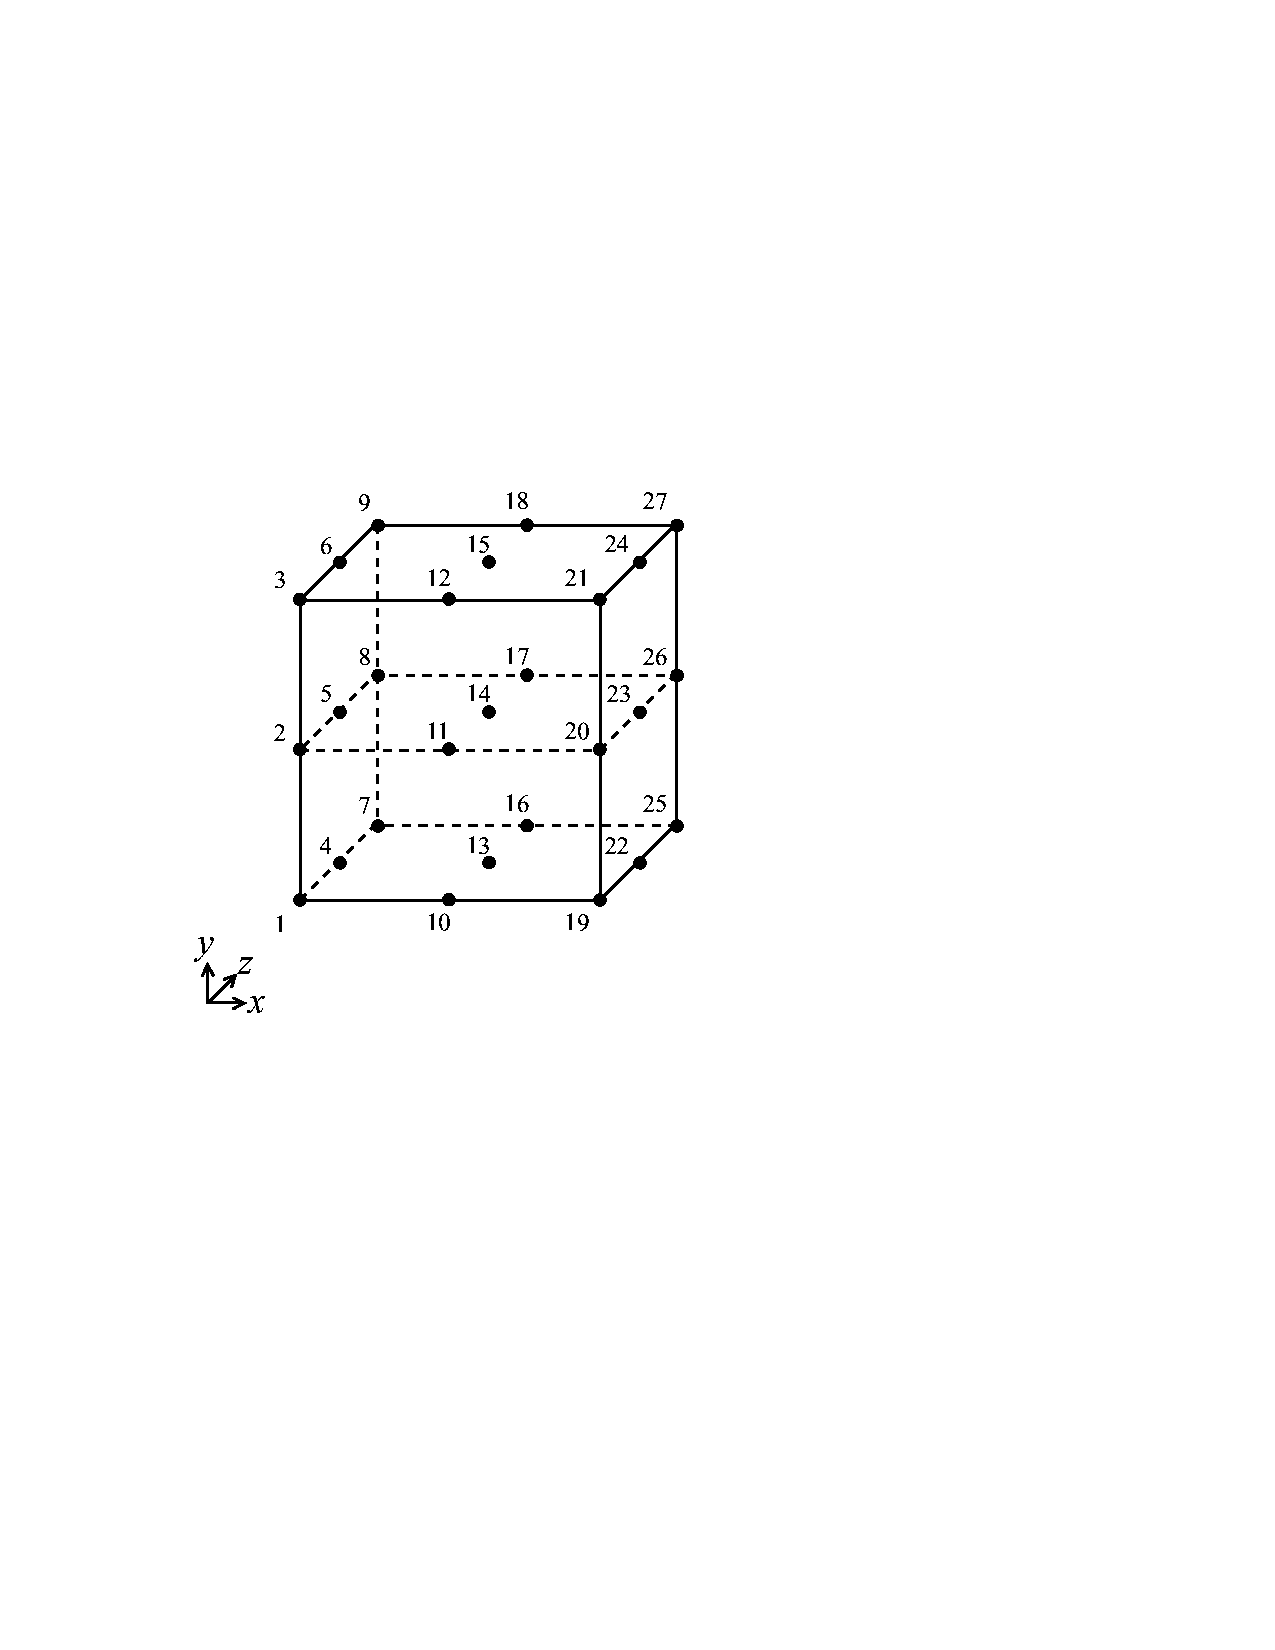
\includegraphics[trim=1.2in 4.2in 3.5in 3.0in, clip, height=2in]{fig/nodeordering3D_27.pdf}
\caption{Node ordering for 8-node and 27-node brick}
\label{fig:NodeOrderingBrick}
\end{figure}

\clearpage
\subsection{Block generators}
\label{section:BlockGenerators}
Thought the methods introduced above for adding nodes and 
elements are general, they can be tedious to use when defining
complicated geometry or for parametric mesh refinement analyses.
Mesh generation can be simplified by using the block generator
commands introduced in this section.

\subsubsection{Simple block generators}
\begin{codelist}
  \item[add\_block(x1,x2,nx,etype,order)]
    The \ttt{add\_block} methods allow you to add a Cartesian strip of
    elements.  This method takes two end points \ttt{x1,x2} and the 
    number of points along the edge (including end points), and constructs 
    a mesh of the strip $[x_{\min}, x_{\max}] \times$.  It is possible to
    remap the bricks later by directly manipulating the mesh \ttt{x}
    array.  Each element has a specified order, and the number of points
    along each edge should be one greater than a multiple of that order.
    Thus \ttt{nx} and \ttt{order} should satisfy the relation,
    \begin{eqnarray}
      \text{nx} &=& \text{order} \times
                    \text{(number of elements between end points)}
                    + 1 \nonumber
    \end{eqnarray}
    The case where we have 7 nodes (\ttt{nx=7}) with varying order of
    elements is shown in Figure \ref{fig:AddBlock1D}.
    \begin{figure}[htbp]
    \centering
    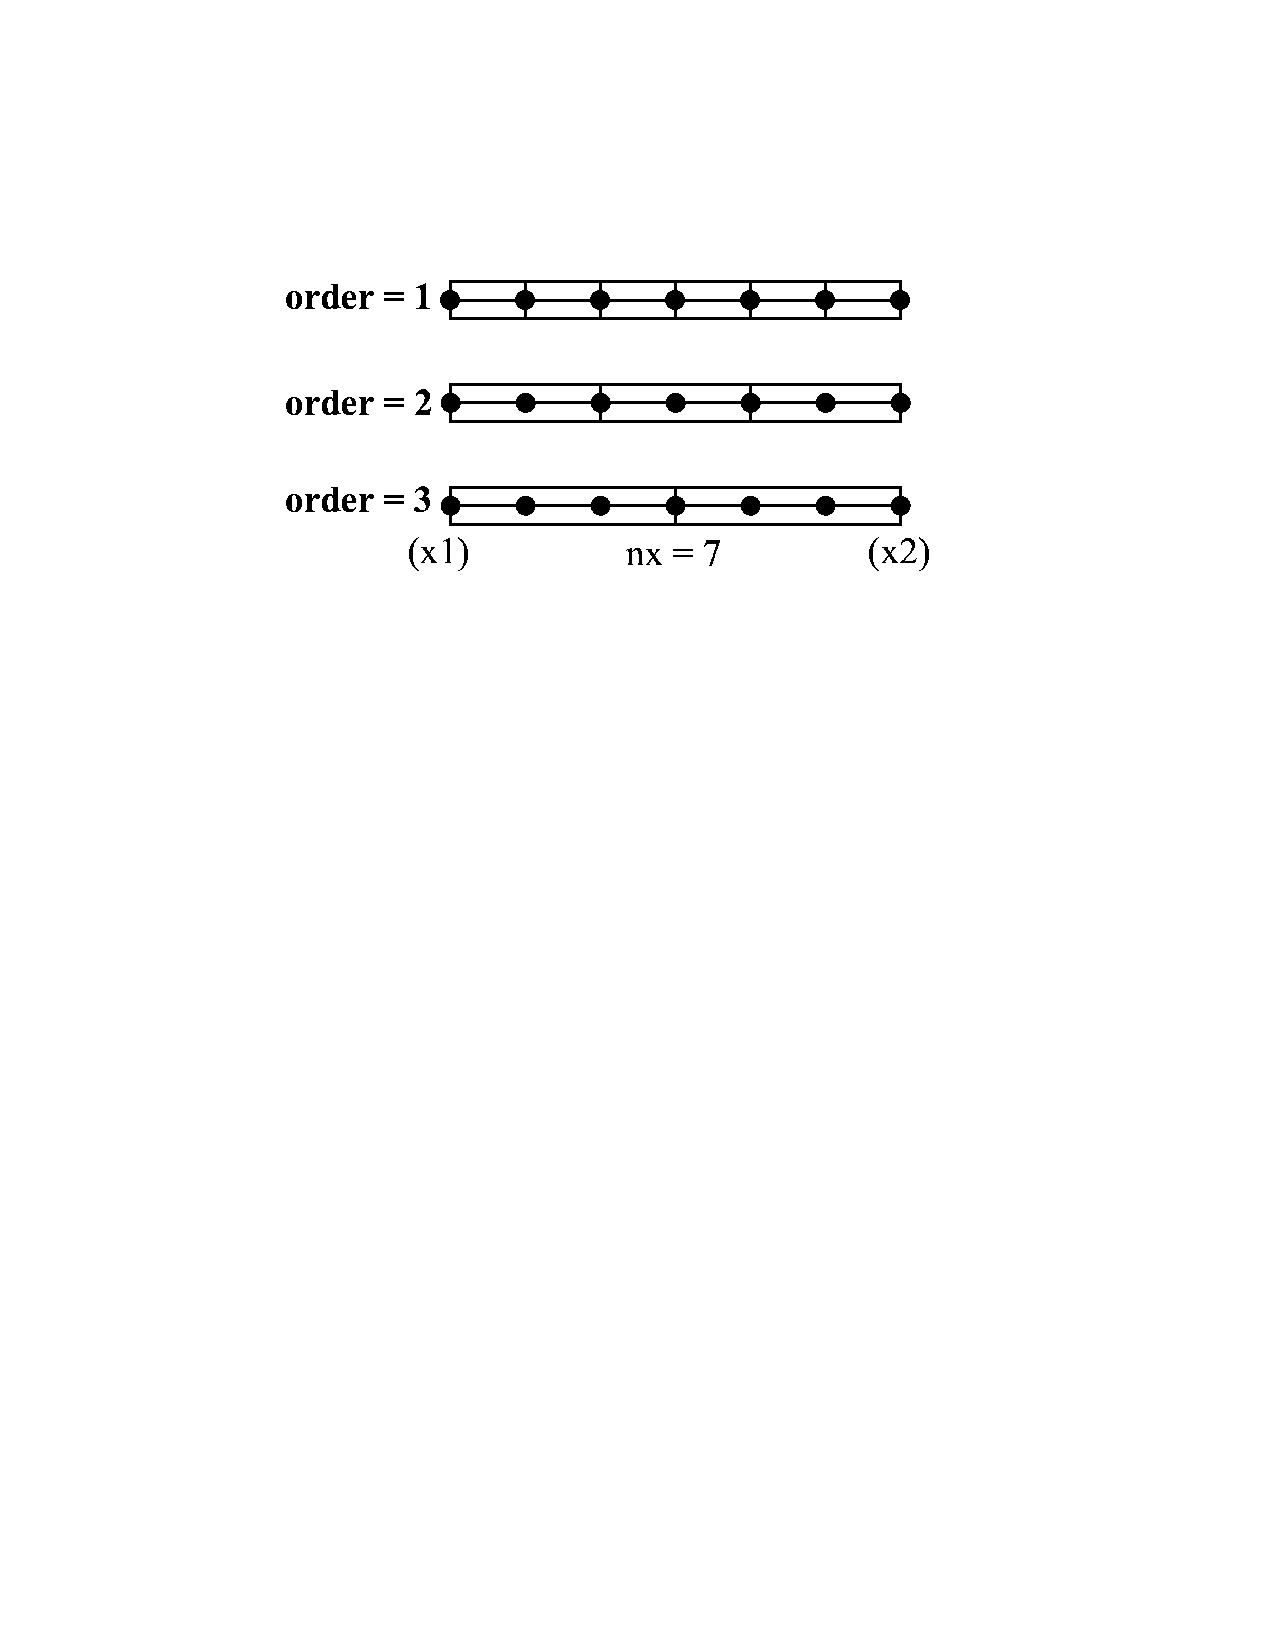
\includegraphics[trim=1.5in 6.5in 2.0in 1.6in, clip, height=2in]{fig/add_blocks1d.pdf}
    \caption{add\_block(x1,x2,nx=7,etype,order=1,2,3)}
    \label{fig:AddBlock1D}
    \end{figure}

\clearpage
  \item[add\_block(x1,y1,x2,y2,nx,ny,etype,order)]
    This is a 2D version of the \ttt{add\_block} generator.

    The case where we have 7 nodes (\ttt{nx=7}) by 3 nodes (\ttt{ny=3}) 
    with varying order of elements is shown in Figure \ref{fig:AddBlock2D}.
    We see here in this case that \ttt{nx,ny} both must satisfy the relation,
    \begin{eqnarray}
      \text{nx} &=& \text{order} \times
                    \text{(number of elements between end points)}
                    + 1 \nonumber \\
      \text{ny} &=& \text{order} \times
                    \text{(number of elements between end points)}
                    + 1 \nonumber
    \end{eqnarray}
    \begin{figure}[htbp]
    \centering
    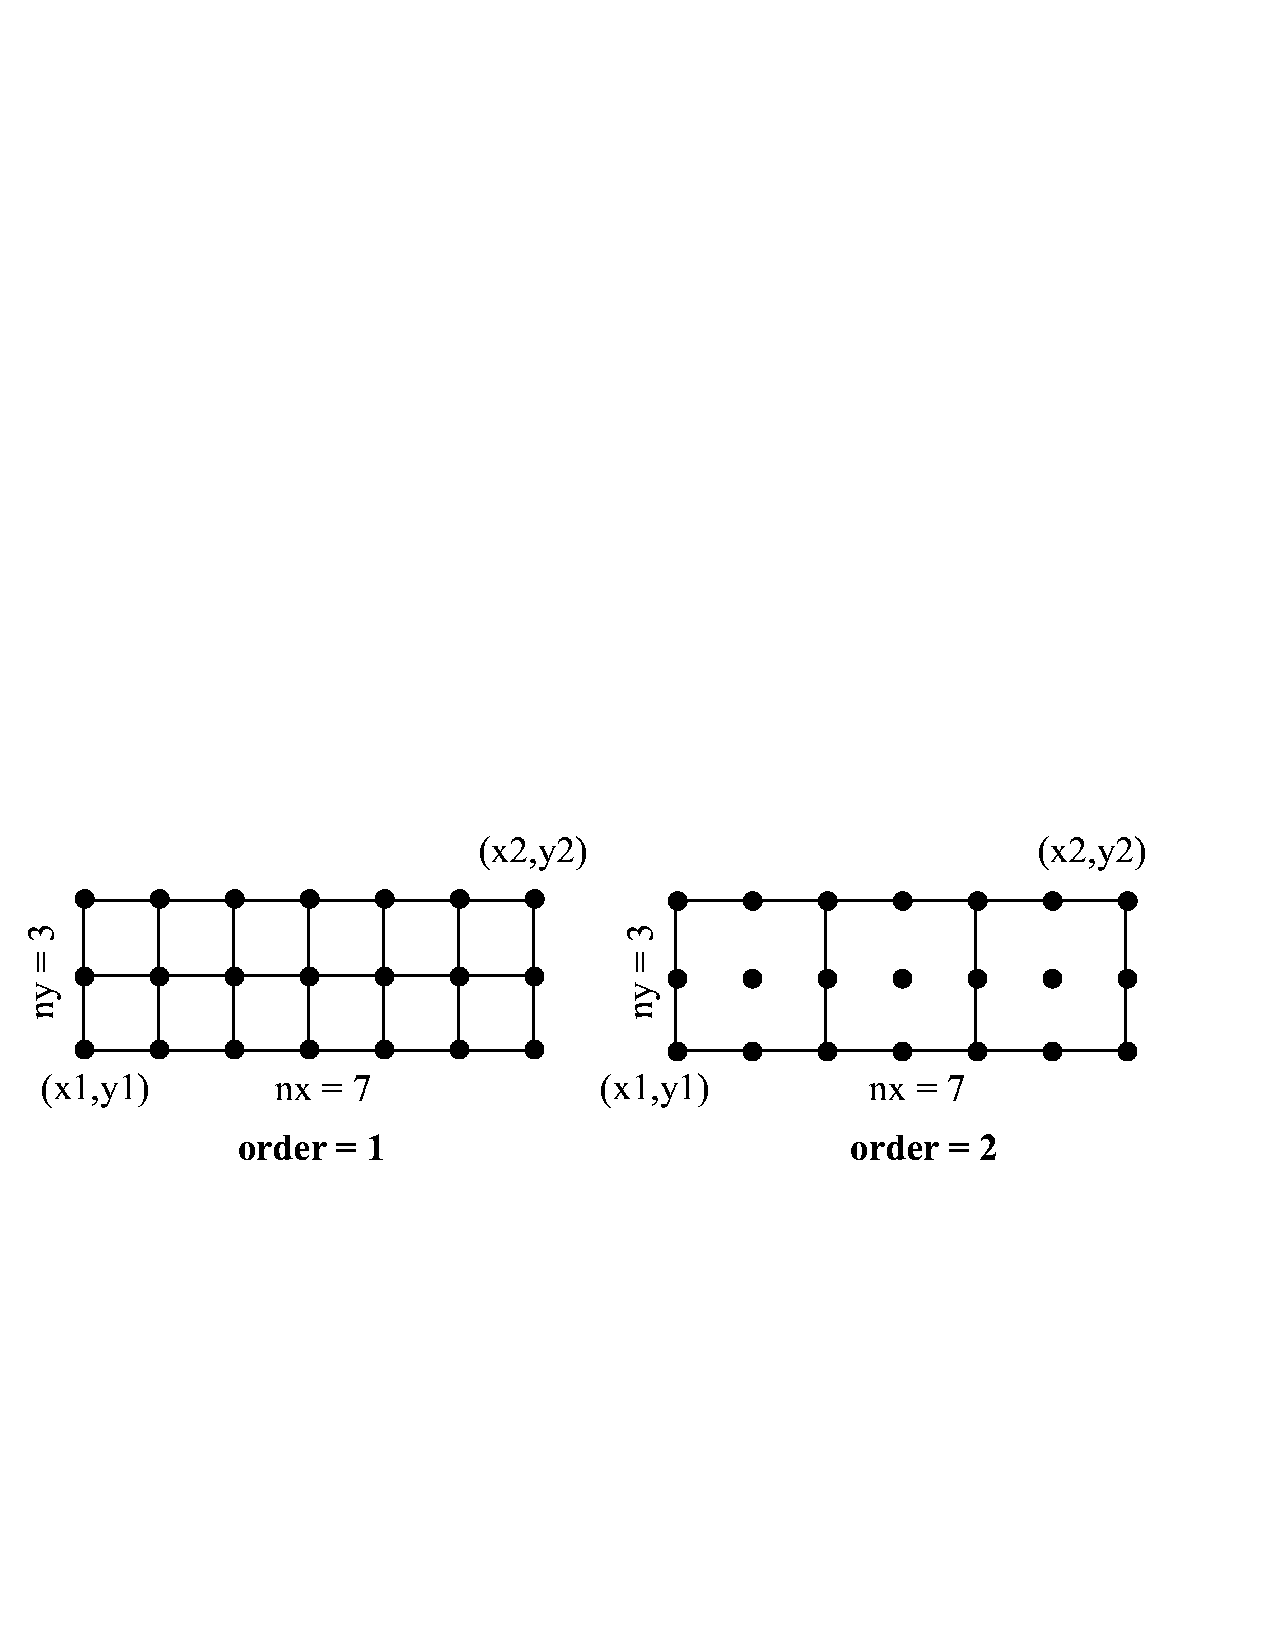
\includegraphics[trim=0.0in 3.0in 0.5in 5.3in, clip, height=1.7in]{fig/add_blocks2d.pdf}
    \caption{add\_block(x1,y1,x2,y2,nx=7,ny=3,etype,order=1,2)}
    \label{fig:AddBlock2D}
    \end{figure}

  \item[add\_block(x1,y1,z1,x2,y2,z2,nx,ny,nz,etype,order)]
    This is a 3D version of the \ttt{add\_block} generator. 
\end{codelist}

\clearpage
\subsubsection{Multiple block generators}
The block generators listed in this section can be understood 
as conducting multiple \ttt{add\_blocks} simultaneously.
This is done by passing an array of controls points along each edge,
and specifying the number of nodes along the edge between these
control points.
\begin{codelist}
  \item[blocks1dn(xlist,rlist,etype,order)]
    Creates a 1D strip of elements with specified nodes
    along the edge \ttt{xlist=\{x$_1$,...,x$_m$    \}}, and specified
    number of nodes along the edge between specified nodes
                   \ttt{rlist=\{r$_1$,...,r$_{m-1}$\}}.
    \ttt{r$_k$}($k=1,\ldots,m-1$) and \ttt{order} must satisfy the 
    relation stated in the generator \ttt{add\_block}. 

    The case where we have 3 control nodes, with 5 and 3 nodes along
    the edges between these nodes and varying order of elements, 
    is shown in Figure \ref{fig:Blocks1dn}.
    \begin{figure}[htbp]
    \centering
    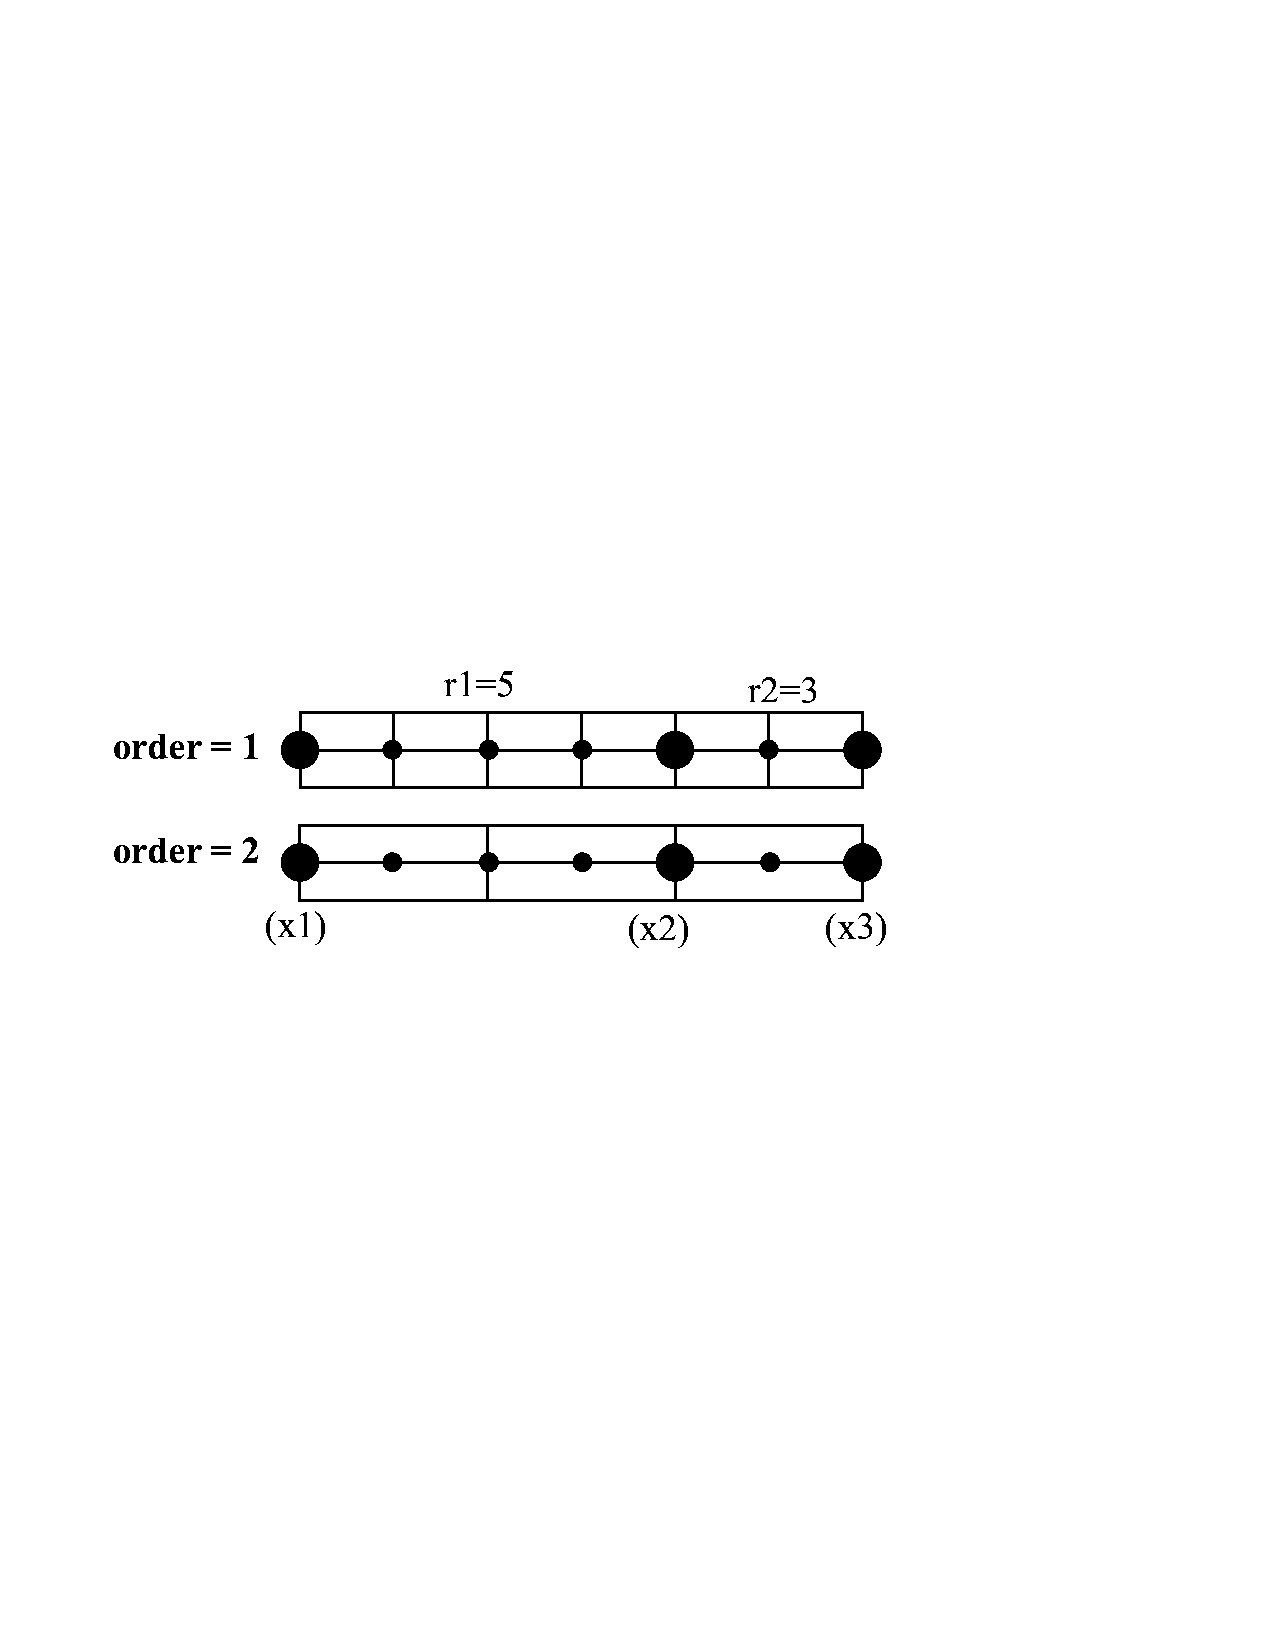
\includegraphics[trim=0.0in 4.5in 2.0in 4.2in, clip, height=1.5in]{fig/blocks1dn.pdf}
    \caption{blocks1dn(\{x1,x2,x3\},\{r1=5,r2=3\},etype,order=1,2)}
    \label{fig:Blocks1dn}
    \end{figure}

  \item[blocks2dn(xlist,rlist,ylist,slist,etype,order)]
    Creates a 2D block of elements with specified nodes
    along the edges 
    \ttt{xlist=\{x$_1$,...,x$_m$    \}}, 
    \ttt{ylist=\{y$_1$,...,y$_n$    \}}, and specified
    number of nodes along each edge between specified nodes
                   \ttt{rlist=\{r$_1$,...,r$_{m-1}$\}},
                   \ttt{slist=\{s$_1$,...,s$_{n-1}$\}}.
    Both \ttt{r$_k$}($k=1,\ldots,m-1$),\ttt{s$_k$}($k=1,\ldots,n-1$) 
    and \ttt{order} must satisfy the relation stated in the generator 
    \ttt{add\_block}. 

  \item[blocks3dn(xlist,rlist,ylist,slist,zlist,tlist,etype,order)]
    Creates a 3D block of elements with specified nodes
    along the edges 
    \ttt{xlist=\{x$_1$,...,x$_m$    \}}, 
    \ttt{ylist=\{y$_1$,...,y$_n$    \}}, 
    \ttt{zlist=\{z$_1$,...,z$_p$    \}}, and specified
    number of nodes along each edge between specified nodes
                   \ttt{rlist=\{r$_1$,...,r$_{m-1}$\}},
                   \ttt{slist=\{s$_1$,...,s$_{n-1}$\}},
                   \ttt{tlist=\{t$_1$,...,t$_{p-1}$\}}.
    Both \ttt{r$_k$}($k=1,\ldots,m-1$),\ttt{s$_k$}($k=1,\ldots,n-1$),
         \ttt{t$_k$}($k=1,\ldots,p-1$) 
    and \ttt{order} must satisfy the relation stated in the generator 
    \ttt{add\_block}. 
\end{codelist}

\newpage
\begin{codelist}
  \item[blocks1d(xlist,etype,order,dense1)]
    Creates a 1D strip of elements with specified nodes
    along the edge \ttt{xlist=\{x$_1$,...,x$_m$    \}}. Nodes
    are inserted between these nodes according to the parameter
    \ttt{dense1}, which specifies the approximate size of the
    element. The method will fit $r_k$ number of elements with
    \ttt{order} between the specified nodes, where $r_k~~(k=1,\ldots,m-1)$ 
    is defined by the equation,
    \begin{eqnarray}
    r_k &=& \text{order} * \text{ceil}\left(\frac{x_{k+1}-x_k}
                                                 {\text{dense1}}\right)
                         + 1~. \nonumber
    \end{eqnarray} 
    The function \text{ceil} rounds to the nearest integer towards infinity.
    If the parameter \ttt{order} or \ttt{dense1} is not specified, the
    method will look for a global variable with the name \ttt{order} and
    \ttt{dense}. If these are supplied, the method will execute with no
    error.  

    The case where we have 3 control nodes with specified \ttt{dense1} 
    is shown in Figure \ref{fig:Blocks1d}. Since the number of elements is
    specified by \ttt{dense1}, we can see that as we increase the order of 
    each element, the number of nodes increases. 
    \begin{figure}[htbp]
    \centering
    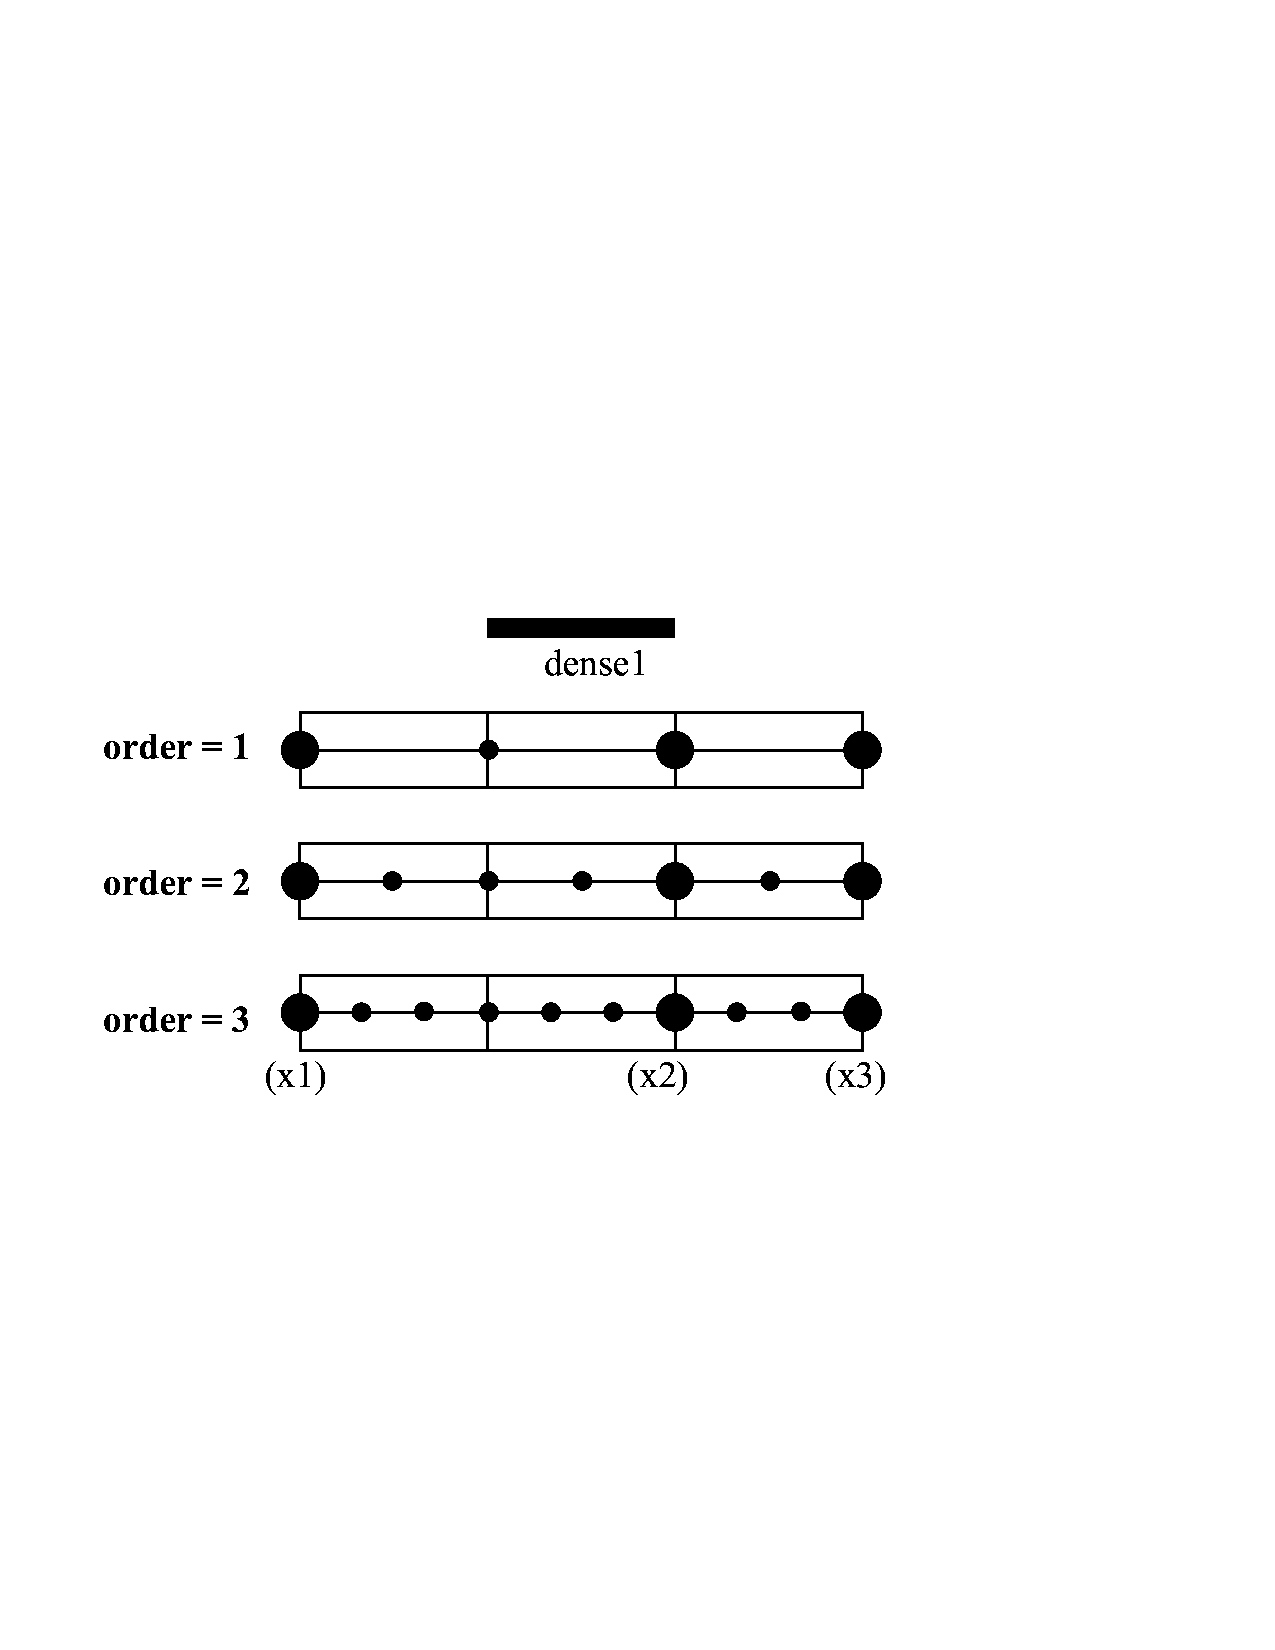
\includegraphics[trim=0.0in 3.5in 2.0in 4.0in, clip, height=1.7in]{fig/blocks1d.pdf}
    \caption{blocks1d(x=\{x1,x2,x3\},etype,order=1,2,3,dense1)}
    \label{fig:Blocks1d}
    \end{figure}
\end{codelist}
\clearpage
\begin{codelist} 
 \item[blocks2d(xlist,ylist,etype,order,dense1,dense2)]
    Creates a 2D block of elements with specified nodes
    along the edge 
    \ttt{xlist=\{x$_1$,...,x$_m$    \}},
    \ttt{ylist=\{y$_1$,...,y$_n$    \}}.
    Nodes are inserted between these nodes according to the parameter
    \ttt{dense1,dense2}, which specify the approximate size of the
    element. The method will fit $r_k$ number of elements in the $x$
    direction with \ttt{order} between the specified nodes, 
    and $s_k$ number of elements in the $y$
    direction with \ttt{order} between the specified nodes,
    where $r_k~~(k=1,\ldots,m-1)$, $s_k~~(k=1,\ldots,n-1)$ 
    is defined by the equation,
    \begin{eqnarray}
    r_k &=& \text{order} * \text{ceil}\left(\frac{x_{k+1}-x_k}
                                                 {\text{dense1}}\right)
                         + 1   \nonumber \\
    s_k &=& \text{order} * \text{ceil}\left(\frac{y_{k+1}-y_k}
                                                 {\text{dense2}}\right)
                         + 1~. \nonumber
    \end{eqnarray} 
    The function \text{ceil} rounds to the nearest integer towards infinity.
    If the parameter \ttt{order} or \ttt{dense1} \ttt{dense2} is not 
    specified, the method will look for a global variable with the name 
    \ttt{order} and \ttt{dense}. If these are supplied, the method will 
    assume \ttt{order = order }, \ttt{dense1 = dense}, and \ttt{dense2 = dense}
    and execute with no error.  

    The case where we have 3 control nodes along the $x$ direction and 
    2 control nodes along the $y$ direction with specified \ttt{dense1,dense2} 
    is shown in Figure \ref{fig:Blocks2d}. Since the number of elements is
    specified by \ttt{dense1,dense2}, we can see that as we increase the 
    order of each element, the number of nodes increases. 
    \begin{figure}[htbp]
    \centering
    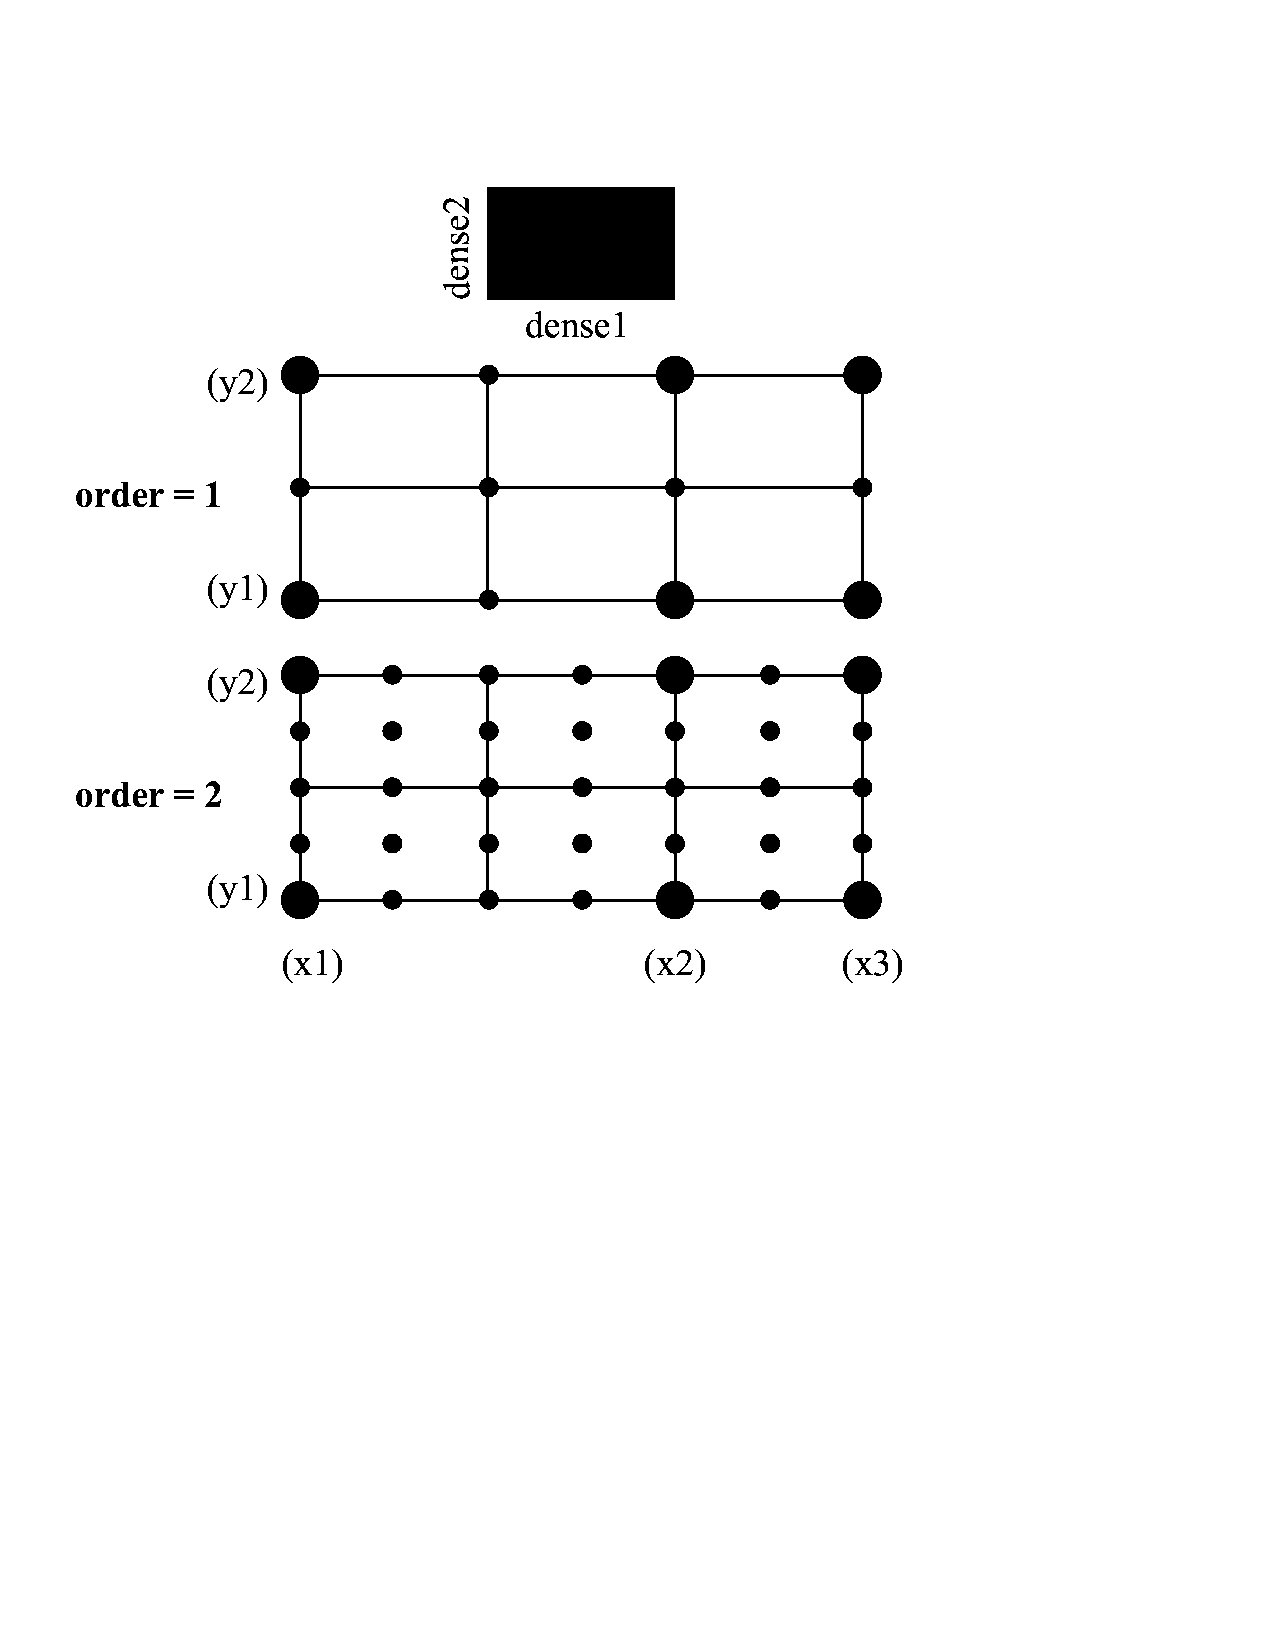
\includegraphics[trim=0.0in 4.5in 2.5in 1.0in, clip, height=2.5in]{fig/blocks2d.pdf}
    \caption{blocks2d(m=3,n=4,etype,order=1,func)}
    \caption{blocks2d(x=\{x1,x2,x3\},y=\{y1,y2\},etype,order=1,2,dense1,dense2)}
    \label{fig:Blocks2d}
    \end{figure}
  \item[blocks3d(xlist,ylist,zlist,etype,order,dense1,dense2,dense3)]
    Creates a 3D block of elements with specified nodes
    along the edge. 3D version of the function above. 

\end{codelist}

\clearpage
\subsubsection{Transformed block generation in Lua}
The block generators introduced in the previous two sections
are limitted to constructing square rectanglur mesh regions
which lacks flexibility. The generators presented in this 
section are versions of the \ttt{add\_block} command which can 
construct curved or non-rectangular blocks.
\begin{codelist}
  \item[add\_block\_shape(m,n,p,etype,order,pts)] 
    Creates a 3D (or 2D if \ttt{p} is omitted) quad block with node
    positions on $[-1,1]^ndm$ and transforms them using an isoparametric
    mapping with points specified in the \ttt{pts} array.  For
    example, for \ttt{pts = \{0,0, 0,1, 1,0, 1,1\}}, we would get a
    mesh for $[0,1]^2$.
    \ttt{m,n,p} and \ttt{order} must satisfy the relation stated in the 
    generator \ttt{add\_block}. 

    An example of a $[-1,1]^2$ region with 3 nodes along the x direction and
    4 nodes along the y direction mapped to a 4-noded polygon with 
    specified nodal points is presented in Figure \ref{fig:AddBlockShape}.
    \begin{figure}[htbp]
    \centering
    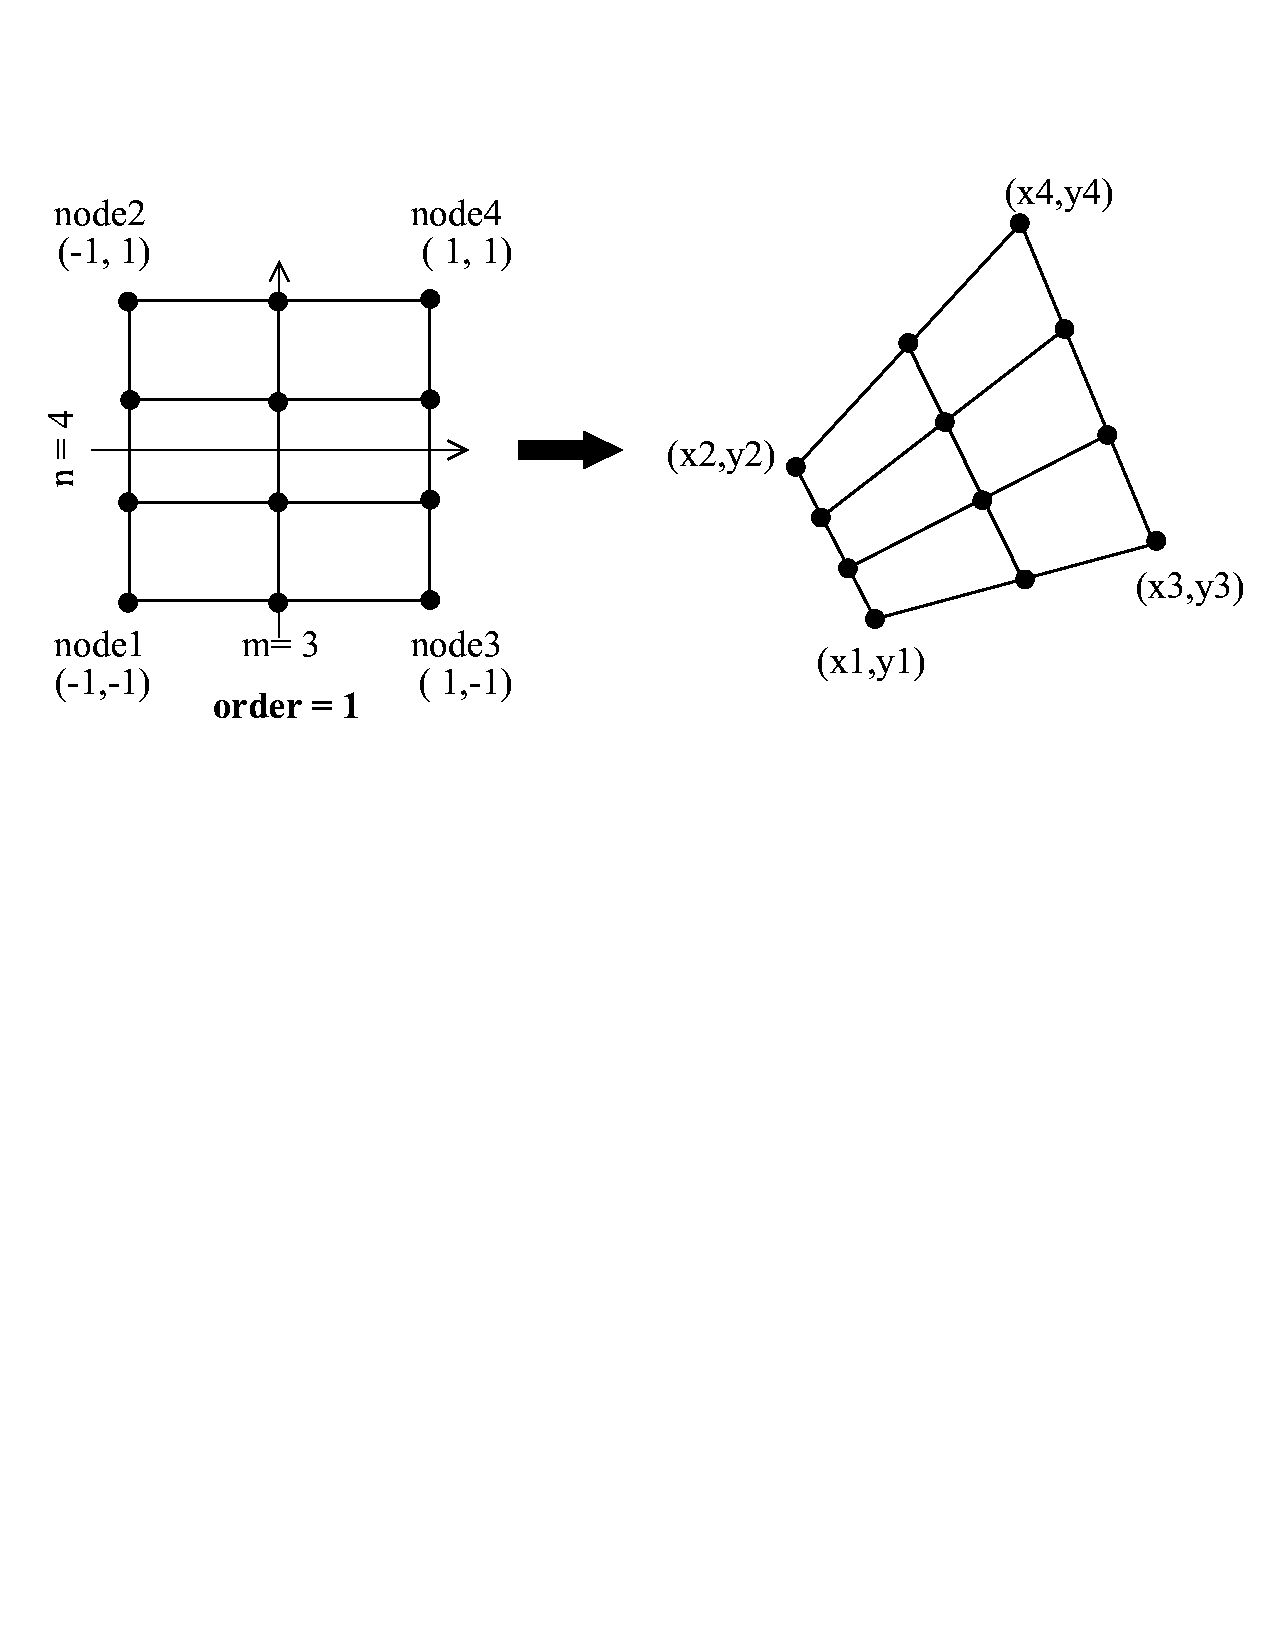
\includegraphics[trim=0.0in 5.5in 0.0in 1.0in, clip, height=1.7in]{fig/block_shape.pdf}
    \caption{add\_\_block\_shape(m=3,n=4,etype,order=1,pts)}
    \label{fig:AddBlockShape}
    \end{figure}

  \item[add\_block\_transform(m,n,p,etype,order,func)] 
    Creates a 3D (or 2D if \ttt{p} is omitted) quad block with node
    positions on $[-1,1]^ndm$ and transforms them using the specified
    function. The function \ttt{func} must have the following form for 2D,
    \begin{verbatim}
       function func(x,y)
         -- Compute mapped coordinates (new_x,new_y) from (x,y)
         return new_x,new_y
       end
    \end{verbatim}
    and for 3D,
    \begin{verbatim}
       function func(x,y,z)
         -- Compute mapped coordinates (new_x,new_y,new_z) from (x,y,z)
         return new_x,new_y,new_z
       end
    \end{verbatim}
    \ttt{m,n,p} and \ttt{order} must satisfy the relation stated in the 
    generator \ttt{add\_block}. 

    An example of a $[-1,1]^2$ region with 3 nodes along the x direction and
    4 nodes along the y direction mapped to a curved block according to a 
    polar mapping is presented in Figure \ref{fig:AddBlockTransform}.
    \begin{figure}[htbp]
    \centering
    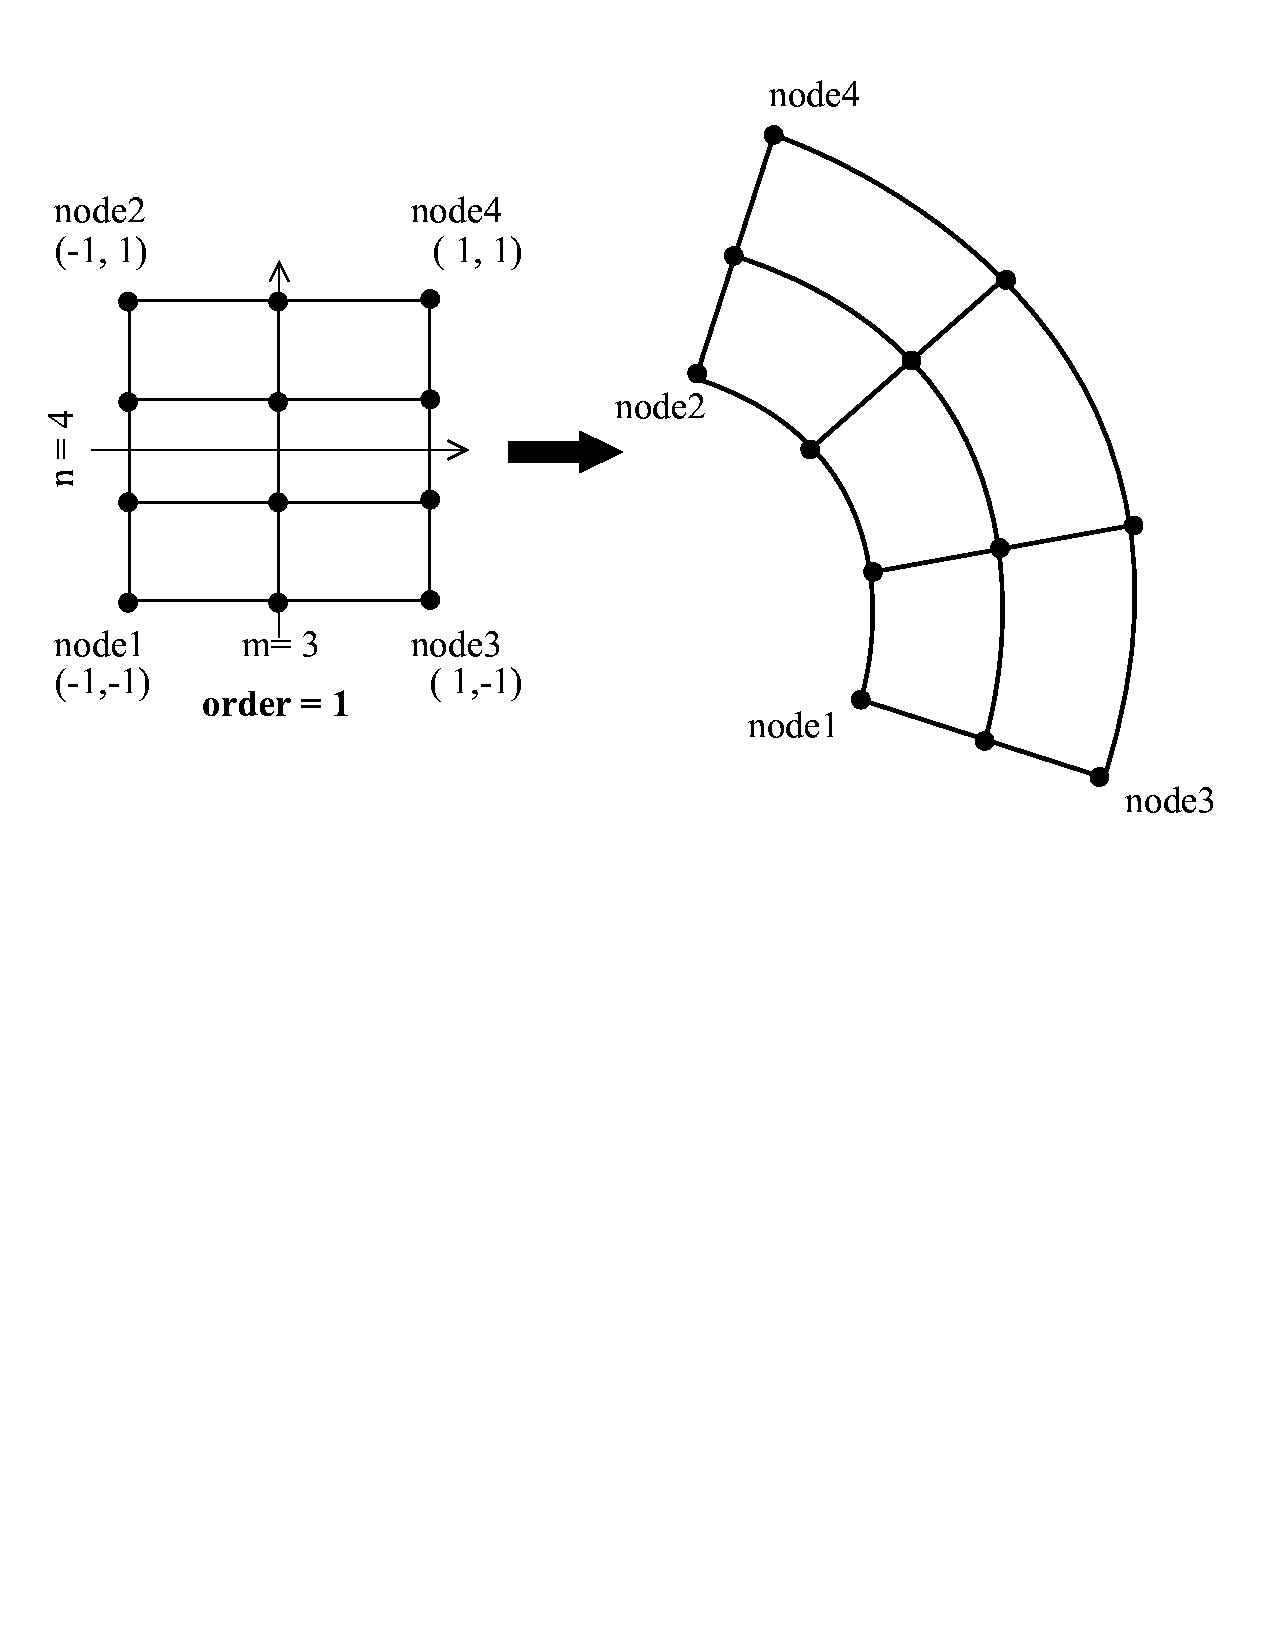
\includegraphics[trim=0.0in 5.5in 0.0in 0.5in, clip, height=1.7in]{fig/block_transform.pdf}
    \caption{add\_\_block\_transform(m=3,n=4,etype,order=1,func)}
    \label{fig:AddBlockTransform}
    \end{figure}

  \item[add\_curved\_block\_shape2d(m,n,etype,order,pts,curv)]
    Creates a 2D quad block with nodes positions on $[-1,1]^2$, 
    \ttt{m} node points along the $x$ direction and \ttt{n} node
    points along the $y$ direction, both including edge points. 
    \ttt{m,n} and \ttt{order} must satisfy the relation stated in
    the generator \ttt{add\_block}. The nodes on the corner of the 
    quad block are mapped to the 4 node points stored in the table
    \ttt{pts=\{x1,y1,x2,y2,x3,y3,x4,y4\}}. The table 
    \ttt{curv=\{curv1,curv2,curv3,curv4\}} contains the curvature
    on each edge, positive values specifying outward curvature and 
    negative values inward curvature.
    \ttt{m,n} and \ttt{order} must satisfy the relation stated in the 
    generator \ttt{add\_block}. 

    An example of a $[-1,1]^2$ region with 3 nodes along the x direction and
    4 nodes along the y direction mapped to a curved block with 4 control
    nodes and various curvatures on the edges is presented in 
    Figure \ref{fig:AddCurvedBlockShape2D}.
    \begin{figure}[htbp]
    \centering
    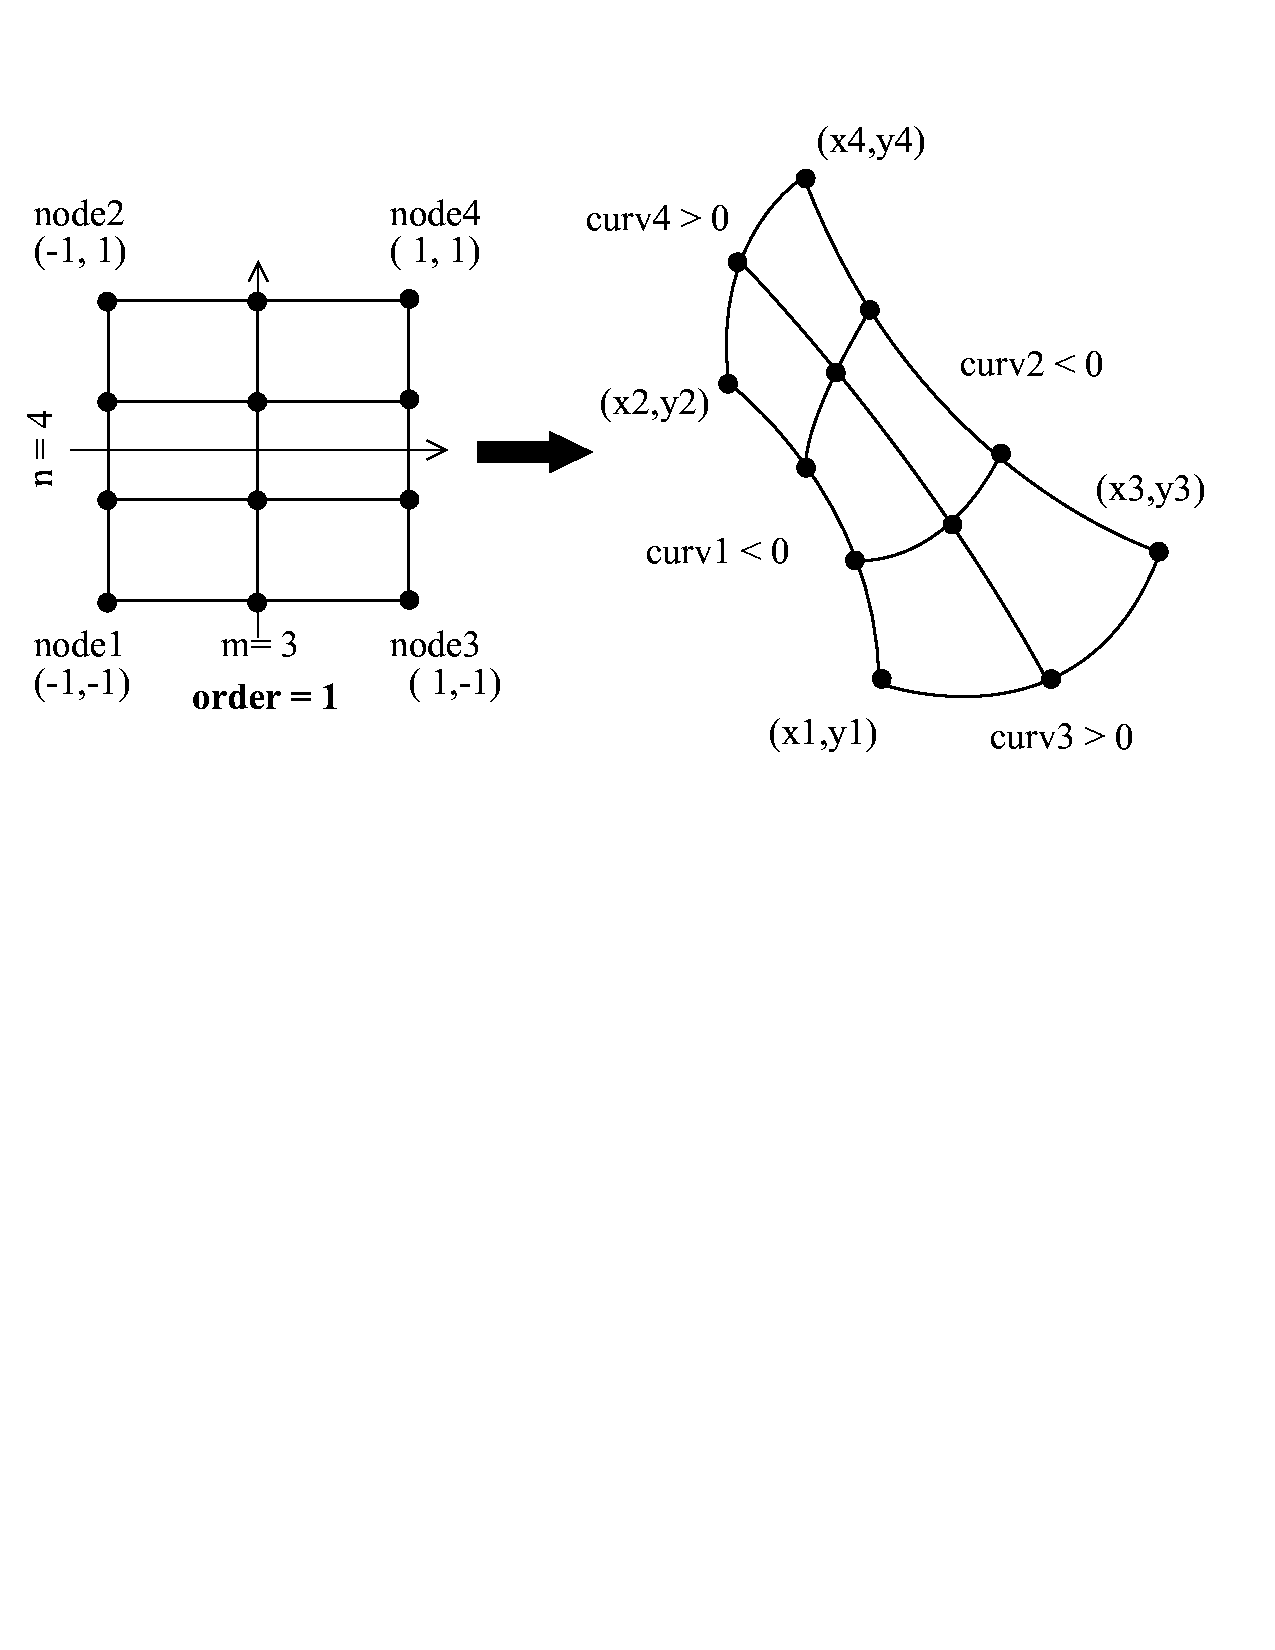
\includegraphics[trim=0.0in 5.5in 0.0in 0.5in, clip, height=1.7in]{fig/block_curved_block.pdf}
    \caption{add\_curved\_block\_shape2d(m=3,n=4,etype,order=1,pts,curv)}
    \label{fig:AddCurvedBlockShape2D}
    \end{figure}
\end{codelist}

\clearpage
\subsection{Tie command}
The mesh class also has a \ttt{tie} method which ``merges'' nodes
which are close to each other.  
\begin{codelist}
  \item[tie(tol)] The \ttt{tie} method takes a
  tolerance \ttt{tol} to try to tie nodes together. If this argument isn't
  specified, the method will look for a global parameter named \ttt{meshtol}.
  When this is given, the method will execute without error.
  If \ttt{tie} finds that nodes $i$ and $j$ in the specified range are
  within the given tolerance of each other, the \ttt{ix} array is
  rewritten so that references to either $i$ or $j$ become references to
  $\min(i,j)$.
\end{codelist}

The \ttt{tie} method acts as though the relation ``node $i$ is
within the tolerance of node $j$'' were an equivalence relation.  But
while this relation is reflexive and symmetric, it does \emph{not}
have to be transitive for general meshes: that is, if $x_i$, $x_j$,
and $x_k$ are three node positions, you might have
\[
  \|x_i - x_j\| < \mathrm{tol} \mbox{ and }
  \|x_j - x_k\| < \mathrm{tol} \mbox{ and }
  \|x_i - x_k\| > \mathrm{tol}.
\]
The behavior of the \ttt{tie} algorithm is undefined in this case.
Make sure it does not happen in your mesh.

\devnote{The right thing to do here is to make the semantics explicit
  (by using the transitive closure of the above relationship, for
  instance) and warn the user if there were any places where the
  behavior of the tie command is not obvious.}

\subsection{Applying boundary conditions}
There are three types of boundary conditions that can be set.
\begin{itemize}
\item Nodal boundary conditions: These are set on the degrees of 
      freedom of each node in the mesh.
\item Global variable boundary conditions: These are set on the 
      global degrees of freedom that can be set. (See section on
      global variables for details).
\item Element variable boundary conditions: These are set on the
      variables that pertain to a specific element. 
\end{itemize}
For each case they are set by specifying functions and passing them
into the mesh through the command,
\begin{codelist}

  \item[set\_bc(func)] Passes a single nodal boundary condition 
  function \ttt{func}.

  \item[set\_bc(func\_table)] Passes a table of nodal boundary condition
  functions \ttt{func\_table=\{func$_1$,$\ldots$,func$_n$\}}.

  \item[set\_globals\_bc(func)] Passes a single global variable boundary 
  condition function \ttt{func}.

  \item[set\_globals\_bc(func\_table)] Passes a table of global variable
  boundary condition functions 
  \ttt{func\_table=\{func$_1$,$\ldots$,func$_n$\}}.

  \item[set\_elements\_bc(func)] Passes a single element variable boundary 
  condition function \ttt{func}.
  
  \item[set\_elements\_bc(func\_table)] Passes a table of element variable
  boundary condition functions 
  \ttt{func\_table=\{func$_1$,$\ldots$,func$_n$\}}.

\end{codelist}

\subsubsection{Nodal boundary conditions}
The Lua function passed to \ttt{set\_bc} should take as input the
coordinates of the nodal point (the number depends on \ttt{ndm}),
and should return a string describing which variables at that node are
subject to force or displacement boundary conditions.  If there are
any nonzero boundary conditions, they should be specified by
additional return arguments.  For example, the following function
applies zero displacement boundary conditions to the first degree of
freedom and nonzero force conditions (of $-1$) to the third degree of
freedom along the line $x = 0$:
\begin{verbatim}
  function bcfunc(x,y)
    if x == 0 then return 'u f', 0, -1; end
  end
\end{verbatim}
If no boundary condition is specified (as occurs at $x \neq 0$ in the
above example), then we assume that there is no boundary condition.
If a boundary condition \emph{is} specified, but without a specific
value, then we assume the corresponding force or displacement should
be zero.  Run time errors result in a user warning, as described in
Section~\ref{section-lua-error-handling}.

The \ttt{bcfunc} defined above is passed to the mesh through the sample
code,
\begin{verbatim}
   mesh:set_bc(bcfunc)
\end{verbatim}

\subsubsection{Global variable boundary conditions}
The Lua function passed to \ttt{set\_globals\_bc} should take as input the
index of the global variable. This index is returned when the global
variable is set to the mesh with the function \ttt{add\_global}.
(See section on global variables for details.)
The function should return a string describing whether the global variable
is subject to a force or displacement boundary condition.  If there are
any nonzero boundary conditions, they should be specified by
additional return arguments.  For example, the following function
applies zero displacement boundary conditions to the global variable
with index equal to 3:
\begin{verbatim}
  function global_variable_bcfunc(ind)
    if ind == 3 then return 'u', 0; end
  end
\end{verbatim}
If no boundary condition is specified then we assume that there 
is no boundary condition.
If a boundary condition \emph{is} specified, but without a specific
value, then we assume the corresponding force or displacement should
be zero.  Run time errors result in a user warning, as described in
Section~\ref{section-lua-error-handling}.

The \ttt{global\_variable\_bcfunc} defined above is passed to the mesh 
through the sample code,
\begin{verbatim}
   mesh:set_globals_bc(global_variable_bcfunc)
\end{verbatim}

\subsubsection{Element variable boundary conditions}
The Lua function passed to \ttt{set\_elements\_bc} should take as input the
number of the element. This number is returned when the element 
is set to the mesh with the function \ttt{add\_element}.
(See section on elements for details.)
The function should return a string describing whether the element variables
are subject to a force or displacement boundary condition.  If there are
any nonzero boundary conditions, they should be specified by
additional return arguments.  For example, the following function
applies a unit forced boundary conditions to the 2nd element variable
of element number 42:
\begin{verbatim}
  function element_variable_bcfunc(elemnum)
    if elemnum == 42 then return ' f', 1; end
  end
\end{verbatim}
If no boundary condition is specified then we assume that there 
is no boundary condition.
If a boundary condition \emph{is} specified, but without a specific
value, then we assume the corresponding force or displacement should
be zero.  Run time errors result in a user warning, as described in
Section~\ref{section-lua-error-handling}.

The \ttt{element\_variable\_bcfunc} defined above is passed to the mesh 
through the sample code,
\begin{verbatim}
   mesh:set_elements_bc(element_variable_bcfunc)
\end{verbatim}

\subsection{Helper Lua commands}
\subsubsection{Numerical value comparison commands}
The methods stated here exist to mitigate the error 
introduced by numerical roundoff errors. When defining
parameters and nodes for mesh information, addition,
multiplication, and division give rise to situations
where a variable $x$ and $y$ take the value,
\begin{verbatim}
   x = 4.0 
   y = 4.000000000000003 
\end{verbatim}
If we compare these two values, the statement
\begin{verbatim}
   x == y
\end{verbatim}
will return false, though actually they are the same value
to the extent that we are interested in. Comparissons of
numerical values such as these arise in boundary condition
functions, pml stretch functions, and many more and can cause
error. This can be alleviated by using the following comparison
functions which take a certain tolerance in the comparison.
For each function, if \ttt{tol} is not specified, it will search
for a global variable named \ttt{meshtol}. If this variable is
found the function will execute properly. 
\begin{codelist}
  \item[mesheq(x,y,tol)] Returns true if $|x-y| < \text{tol}$ and 
  false otherwise. 
  \item[meshleq(x,y,tol)] Returns true if $ x < y + \text{tol}$ and 
  false otherwise.
  \item[meshsl(x,y,tol)] Returns true if $ x < y - \text{tol}$ and 
  false otherwise.
  \item[meshgeq(x,y,tol)] Returns true if $ x + \text{tol} > y$ and
  false otherwise.
  \item[meshsg(x,y,tol)] Returns true if $ x - \text{tol} > y$ and
  false otherwise.
  \item[meshbetween(x,xmin,xmax,tol)] Returns true if 
  $ xmin - \text{tol} < x < xmax + \text{tol}$ and false otherwise.
  \item[meshsbetween(x,xmin,xmax,tol)] Returns true if 
  $ xmin + \text{tol} < x < xmax - \text{tol}$ and false otherwise.
\end{codelist}


\newpage
\section{Global variables}
\label{section:GlobalVariables}
\subsection{Concept of a global variable}
Introducing a global variable can be understood as 
a means to specify constraints among individual 
nodal degrees of freedom much like a lagrange
multiplier. It allows one to specify a mode shape
for selected nodal degrees of freedom and assigns
a general degree of freedom for that mode.

The following simple example of a three degree of
freedom spring mass mechanical system may clarify
this concept. The equation of motion for the system
can be written as,
\begin{eqnarray}
\left[
\begin{array}{ccc}
m_1 & 0   & 0   \\
0   & m_2 & 0   \\
0   & 0   & m_3 
\end{array}
\right]
\left(
\begin{array}{c}
\ddot{u}_1(t) \\
\ddot{u}_2(t) \\
\ddot{u}_3(t)
\end{array}
\right)
+
\left[
\begin{array}{ccc}
k_1+k_2 & -k_2       &    0 \\
-k_2    &  k_2 + k_3 & -k_3 \\
-k_2    &  k_2 - k_3 &  k_3 
\end{array}
\right]
\left(
\begin{array}{c}
{u}_1(t) \\
{u}_2(t) \\
{u}_3(t)
\end{array}
\right)
=
\left(
\begin{array}{c}
{F}_1(t) \\
{F}_2(t) \\
{F}_3(t)
\end{array}
\right)
\end{eqnarray}
or in more compact form,
\begin{eqnarray}
\bfM\ddot{\bfu}(t) + \bfK\bfu(t) &=& \bfF(t)
\end{eqnarray}
If we assume that the 2 and 3 degrees of freedom
are connected by a rigid element, then the
degrees of freedom can be expressed by one 
general degree of freedom as follows,
\begin{eqnarray}
\left(
\begin{array}{c}
{u}_1(t) \\
{u}_2(t) \\
{u}_3(t)
\end{array}
\right)
&=& 
\left(
\begin{array}{c}
1  \\
0  \\
0 
\end{array}
\right)
u_1(t)
+
\left(
\begin{array}{c}
0 \\
1 \\
1
\end{array}
\right)
z(t) \nonumber\\
&=& 
\bfe_1 u_1(t) + \bfV_z z(t) \nonumber\\
&=&
\left[
\begin{array}{cc}
\bfe_1 & \bfV_z
\end{array}
\right]
\left(
\begin{array}{c}
u_1(t) \\
z(t) 
\end{array}
\right) \nonumber\\
&=& 
\bfW 
\left(
\begin{array}{c}
u_1(t) \\
z(t) 
\end{array}
\right) 
\end{eqnarray}
Inserting this expression and restricting the error to be 
orthogonal to this subspace spanned by the column vectors of 
$\bfW$ results in the two degree of freedom system,
\begin{eqnarray}
\bfW^*\bfM\bfW
\left(
\begin{array}{c}
\ddot{u}_1(t) \\
\ddot{z}(t) 
\end{array}
\right) 
+ \bfW^*\bfK\bfW 
\left(
\begin{array}{c}
u_1(t) \\
z(t) 
\end{array}
\right) 
&=& \bfW^*\bfF(t)
\end{eqnarray}
that must be solved. 

\subsection{Creating and defining global variables}
The key to creating a global variable is to construct the
shape vector $\bfV_z$ pertaining to the global variable.
This is conducted by specifying a function which is evaluated at
each nodal degree of freedom, similar to the form of the
nodal boundary conditions without the initial string. There
is also an additional restriction that a number must be assigned
for each nodal degree of freedom. As an example the shape
function for the first example would have the form,
\begin{verbatim}
      function shape_func_global_variable(x)
          if x==2 then return 1; end
          if x==3 then return 1; end
      end
\end{verbatim}

The general constructor for adding global variables to the
mesh is:
\begin{codelist}

  \item[index = Mesh:add\_global(shapeg,s\_1,s\_2)]
  \ttt{shapeg} must be a function of the form presented above.
  The variables \ttt{s\_1,s\_2} are optional and are the nondimensionalization
  parameters for the global variable. They can be numbers or strings
  that are predefined in the table \ttt{dim\_scales}. (See section on
  non-dimensionalization for details). The function returns the \ttt{index}
  of the global variable.

  \item[{Mesh:set\_globals()}]
  Once all the global variables required are added they must be 
  set to the mesh. Unless this function is called, the process will
  not be complete.

\end{codelist}
For the case presented in the previous section adding the global 
variable would take the process,
\begin{verbatim}
      index = mesh:add_global(shape_func_global_variable,'L','F')
      mesh:set_globals()
\end{verbatim}
The value for the strings \ttt{'L'} and \ttt{'F'} must be set
in \ttt{dim\_scales}.



\newpage
\section{Element library}
\label{section:ElementLibrary}
\subsection{PML elements}

\emph{Perfectly matched layers} (PMLs) are what is used to model
the effect of energy loss through supports or anchor loss.
PMLs mimic the effect of an infinite or semi-infinite medium,
by applying complex-value coordinate transformations.
PMLs fit naturally
into a finite element framework, but to implement them, we need some
way to describe the exact form of the coordinate transformation.
This coordinate-stretching function used in a PML is is defined as a
Lua function and set to the set to the element that
the PML is imposed by the following function:
\begin{codelist}

  \item[set\_stretch(stretch\_func)]
    Use a Lua function \ttt{stretch\_func} to describe the coordinate 
    transformation.  
    The coordinate stretching function in 2D should have the form
    \begin{verbatim}
  function stretch_func(x,y)
    -- Compute stretching parameters sx and sy
    return sx, sy
  end
    \end{verbatim}
    If no stretch values are returned, they are assumed to be zero.
    The PML element should stretch the $x$ and $y$ coordinates by
    $(1-is_x)$ and $(1-is_y)$, respectively.  The 3D case is handled
    similarly.

    This function is set to the element in the following manner.
    \begin{verbatim}
  element_to_apply_pml:set_stretch(stretch_func)
    \end{verbatim}

    The stretching function is only ever evaluated at node positions.

\end{codelist}
If there are no calls to either form of \ttt{set\_stretch}, the PML
element does not stretch the spatial coordinate at all, and so the
element behaves exactly like an ordinary (non-PML) element.

For the exact form of this coordinate transformation function and
details in implementation, see the PML example in the Examples
Manual.

\clearpage
\subsection{Laplace elements}

The \ttt{PMLScalar1d}, \ttt{PMLScalar2d}, \ttt{PMLScalar3d}, 
and \ttt{PMLScalarAxis}
classes implement scalar wave equation elements with an optional PML.
The general constructor takes the form,
\begin{codelist}
  \item[etype = make\_material\_s(mtype,analysistype)]
\end{codelist}
The variable \ttt{mtype} must contain the fields
\ttt{rho}(mass density) and \ttt{E}(material stiffness).
The variable \ttt{analysis\_type} can take one of the 
following strings,
\begin{itemize}
\item \ttt{1d}: 1 dimensional analysis
\item \ttt{2d}: 2 dimensional analysis
\item \ttt{3d}: 3 dimensional analysis
\item \ttt{axis}: Axis symmetric analysis
\end{itemize}
The scalar wave equation has the form,
\begin{eqnarray}
\rho \frac{\del^2 u}{\del t^2} &=& 
              \bfnabla\cdot \left( \bkappa \bfnabla u \right)
\end{eqnarray}
where $u$ is the scalar displacement, $\rho$ is the density, 
and $\bkappa$ is the stiffness. 
If no coordinate stretching is 
defined, the elements will generate standard (real) mass and 
stiffness matrices.
The class provides the following constructors:

\begin{codelist}

  \item[PMLScalar1d(kappa,rho)] 
    Creates an isotropic 1D scalar wave equation element with material
    property $\kappa$ and mass density $\rho$.  

  \item[PMLScalar2d(kappa,rho)] 
    Creates an isotropic 2D scalar wave equation element with material
    property $\kappa$ and mass density $\rho$. 

  \item[PMLScalar2d(D,rho)]
    Creates a 2D anisotropic element with a 2-by-2 property matrix
    \ttt{D}.  Other than the material properties, this constructor is
    identical to the previous one.

  \item[PMLScalarAxis(kappa,rho)]
    Creates an isotropic axisymmetric scalar wave equation element
    with material property $\kappa$ and mass density $\rho$.  

  \item[PMLElasticAxis(D,rho)]
    Creates a 2D anisotropic element with a 2-by-2 property matrix
    \ttt{D}.  Other than the material properties, this constructor is
    identical to the previous one.

  \item[PMLScalar3d(kappa,rho)] 
    Creates an isotropic 3D scalar wave equation element with material
    property $\kappa$ and mass density $\rho$.  

  \item[PMLScalar3d(D,rho)]
    Creates a 3D anisotropic element with a 3-by-3 property matrix
    \ttt{D}.  Other than the material properties, this constructor is
    identical to the previous one.

\end{codelist}

\clearpage
\subsection{Elastic elements}

The \ttt{PMLElastic2d}, \ttt{PMLElastic3d}, and \ttt{PMLElasticAxis}
classes implement elasticity (Solid) elements with an optional PML
transformation. 
The general constructor takes the form,
\begin{codelist}
  \item[etype = make\_material\_e(mtype,analysistype)]
  \item[etype = make\_material\_e(mtype, etype, wafer, angle)]
    Constructs and returns a \ttt{PMLElastic} element, depending on the
    given arguments. The material type \ttt{mtype} (string or table containing
    material mechanical properties) and element type
    \ttt{etype}(\ttt{planestrain,planestress,axis,3d}) must be given. 
    The arguments defining wafer orientation \ttt{wafer}(\ttt{'100'} or
    \ttt{'111'}) and orientation angle \ttt{angle} [rad] are optional.
    The table of mechanical properties \ttt{mtype} should contain the 
    fields \ttt{rho, E, nu} for isotropic material, and \ttt{lambda, mu,
    alpha} for cubic material.
    (Currently this element can only treat cubic and isotropic mechanical
     material).
\end{codelist}
The variable \ttt{mtype} must be an elastic materail containing
different fields depending on the symmetry of the crystal considered.
In the case of anisotropic material the second constructor is used,
which defines the wafer orientation and angle.
The variable \ttt{analysis\_type} can take one of the 
following strings,
\begin{itemize}
\item \ttt{planestrain}: 2 dimensional planestrain analysis
\item \ttt{planestress}: 2 dimensional planestress analysis
\item \ttt{3d}: 3 dimensional analysis
\item \ttt{axis}: Axis symmetric analysis
\end{itemize}
These elements solve the following equation,
\begin{eqnarray}
\rho \frac{\del^2 \bfu}{\del t^2}
&=& \bfnabla\cdot\bsig \\
\bsig &=& \bbC:\beps \\
\beps &=& \bfnabla_\text{sym}\bfu
\end{eqnarray}
Here, $\rho$ is the density, $\bsig$ is the stress, $\bbC$ is the
material stiffness tensor, $\beps$ is the infinitesimal strain, and
$\bfu$ is the displacement vector. In the case of an isotropic material,
$\bbC$ will depend only on two variables: the Youngs modulus $E$ and 
Poisson ratio $\nu$. Otherwise the material property can be expressed
by a matrix via Voigt notation. (See section on material models for
further information).
 If no coordinate stretching is 
defined, the elements will generate standard (real) mass and 
stiffness matrices.
The classes provides the following constructors:
\begin{codelist}

  \item[PMLElastic2d(E,nu,rho,plane\_type)]
    Creates a plane strain (\ttt{plane\_type = 0}) or plane stress
    (\ttt{plane\_type = 1}) isotropic elasticity element with
    Young's modulus \ttt{E}, Poisson ratio \ttt{nu}, and mass
    density \ttt{rho}.  

  \item[PMLElastic2d(D,rho)]
    Creates a 2D element with a 3-by-3 elastic property matrix
    \ttt{D}.  Other than the elastic properties, this constructor
    is identical to the previous one.

  \item[PMLElastic2d(lua\_State* L, lua\_Object func)]
    Creates a 2D element with material parameters defined by a
    Lua function \ttt{func}. This function is accessed via the 
    Lua state \ttt{L}. \ttt{func} must take one of the following
    forms. 
    \begin{verbatim}
  function material_function(x,y)
    -- Compute 3-by-3 elastic property matrix D and 
    --                mass density rho
    return D, rho
  end
    \end{verbatim}
    or,
    \begin{verbatim}
  function material_function(x,y)
    -- Compute Young's modulus E, Poisson ration nu, 
    --         mass density rho, and analysis plane_type
    return E, nu, rho, plane_type
  end
    \end{verbatim}
  
  \item[PMLElasticAxis(E,nu,rho)]
    Creates an isotropic axisymmetric elasticity element with
    Young's modulus \ttt{E}, Poisson ratio \ttt{nu}, and mass
    density \ttt{rho}.  

  \item[PMLElasticAxis(D,rho)]
    Creates an element with a 4-by-4 elastic property matrix
    \ttt{D}.  Other than the elastic properties, this constructor
    is identical to the previous one.

  \item[PMLElasticTAxis(E,nu,rho,ltheta)]
    Creates an isotropic axisymmetric elasticity element with
    Young's modulus \ttt{E}, Poisson ratio \ttt{nu}, mass
    density \ttt{rho}, and wave number \ttt{ltheta}.

  \item[PMLElasticTAxis(D,rho,ltheta)]
    Creates an element with a 6-by-6(????) elastic property matrix
    \ttt{D}.  Other than the elastic properties, this constructor
    is identical to the previous one.

  \item[PMLElastic3d(E,nu,rho)] 
    Creates an isotropic 3D elasticity element with Young's modulus
    \ttt{E}, Poisson ratio \ttt{nu}, and mass density
    \ttt{rho}.  

  \item[PMLElastic3d(D,rho)]
    Creates an element with a 6-by-6 elastic property matrix
    \ttt{D}.  Other than the elastic properties, this constructor
    is identical to the previous one.

\end{codelist}

\clearpage
\subsection{Thermoelastic Elements}

The \ttt{PMLElastic2d\_te}, \ttt{PMLElastic3d\_te}, 
and \ttt{PMLElasticAxis\_te}
classes implement thermoelasticity (Solid) elements with an optional PML
transformation. 
The general constructor takes the form,
\begin{codelist}
  \item[etype = make\_material\_te(mtype,analysistype)]
  \item[etype = make\_material\_te(mtype,analysistype,wafer,angle)]
    Constructs and returns a \ttt{PMLElastic\_te} element, depending on the
    given arguments. The material type \ttt{mtype} (string or table containing
    material thermomechanical properties) and element type
    \ttt{etype}(\ttt{planestrain,planestress,axis,3d}) must be given. 
    The arguments defining wafer orientation \ttt{wafer}(\ttt{'100'} or
    \ttt{'111'}) and orientation angle \ttt{angle} [rad] are optional.
    The table of thermomechanical properties \ttt{mtype} should contain the 
    fields \ttt{rho, E, nu} for isotropic material, and \ttt{lambda, mu,
    alpha} for cubic material. For both cases it should contain the fields
    \ttt{at, cp, kt} and \ttt{T0}.
    (Currently this element can only treat cubic and isotropic thermomechanical
     material).
\end{codelist}
The variable \ttt{mtype} must be an elastic materail containing
different fields depending on the symmetry of the crystal considered.
In the case of anisotropic material the second constructor is used,
which defines the wafer orientation and angle.
The variable \ttt{analysis\_type} can take one of the 
following strings,
\begin{itemize}
\item \ttt{planestrain}: 2 dimensional planestrain analysis
\item \ttt{planestress}: 2 dimensional planestress analysis
\item \ttt{3d}: 3 dimensional analysis
\item \ttt{axis}: Axis symmetric analysis
\end{itemize}
These elements solve the following coupled equation,
\begin{eqnarray}
\rho \frac{\del^2 \bfu}{\del t^2}
&=& \bfnabla\cdot\bsig \\
\rho c_v \dot{\theta} 
&=& \bfnabla\cdot\left(\bkappa_T\bfnabla \theta\right)
   - T_0 \dot{\beps}:\bbC:\balpha_T\\
\bsig &=& \bbC:\left(\beps - \balpha_T \theta \right)\\
\beps &=& \bfnabla_\text{sym}\bfu
\end{eqnarray}
Here, $\rho$ is the density, $\bsig$ is the stress, $\bbC$ is the
material stiffness tensor, $\beps$ is the infinitesimal strain, 
$\bfu$ is the displacement vector and $\theta$ is the temperature
fluctuation from $T_0$, which is the referential temperature.
In the case of an isotropic material,
$\bbC$ will depend only on two variables: the Youngs modulus $E$ and 
Poisson ratio $\nu$. In the case of a cubic material, it will depend
on three variables: $\lambda$, $\mu$, and $\alpha$.  In both cases 
the material property can be expressed by a matrix via Voigt notation. 
(See section on material models for further information). The constants
related with the thermal field are, $\bkappa_T$ the thermal conductivity
tensor, $c_v$ the specific heat at constant volume, and $\balpha_T$ which
is the linear coefficient of thermal expansion tensor. 
If no coordinate stretching is defined, the elements will generate 
standard (real) mass and stiffness matrices.
The classes provides the following constructors:
\begin{codelist}
  \item[PMLElastic2d\_te(E,nu,rho,at,cp,kt,T0,plane\_type)]
    Creates a plane strain (\ttt{plane\_type = 0}) or plane stress
    (\ttt{plane\_type = 1}) isotropic thermoelasticity element with
    Young's modulus \ttt{E}, Poisson ratio \ttt{nu}, mass
    density \ttt{rho}, coefficient of thermal expansion \ttt{at},
    thermal capacity at constant pressure \ttt{cp}, thermal conductivity
    at \ttt{kt}, and reference temperature \ttt{T0}.

  \item[PMLElastic2d\_te(Db,rho,at,cp,kt,T0)]
    Creates a 2D element with a 4-by-4 thermoelastic property matrix
    \ttt{D}.  Other than the thermoelastic properties, this constructor
    is identical to the previous one.

  \item[PMLElastic3d\_te(E,nu,rho,at,cp,kt,T0)]
    Creates an isotropic 3D thermoelasticity element with Young's modulus
    \ttt{E}, Poisson ratio \ttt{nu}, mass density \ttt{rho},
    coefficient of thermal expansion \ttt{at},
    thermal capacity at constant pressure \ttt{cp}, thermal conductivity
    at \ttt{kt}, and reference temperature \ttt{T0}.

  \item[PMLElastic3d\_te(Db,rho,at,cp,kt,T0)]
    Creates a 3D element with a 7-by-7 thermoelastic property matrix
    \ttt{D}.  Other than the thermoelastic properties, this constructor
    is identical to the previous one.

  \item[PMLElasticAxis\_te(E,nu,rho,at,cp,kt,T0)]
    Creates an isotropic axisymmetric elasticity element with
    Young's modulus \ttt{E}, Poisson ratio \ttt{nu}, mass density \ttt{rho},
    coefficient of thermal expansion \ttt{at},
    thermal capacity at constant pressure \ttt{cp}, thermal conductivity
    at \ttt{kt}, and reference temperature \ttt{T0}.

  \item[PMLElasticAxis\_te(Db,rho,at,cp,kt,T0)]
    Creates an element with a 5-by-5 thermoelastic property matrix
    \ttt{D}.  Other than the thermoelastic properties, this constructor
    is identical to the previous one.
\end{codelist}

\clearpage
\subsection{Piezoelectric elements}
The \ttt{PMLElastic2d\_pz}, \ttt{PMLElastic3d\_pz}, 
and \ttt{PMLElasticAxis\_pz}
classes implement piezoelectric elasticity (Solid) elements with an 
optional PML transformation. 
The general constructor takes the form,
\begin{codelist}
  \item[etype = make\_material\_pz(mtype,analysistype)]
  \item[etype = make\_material\_pz(mtype,analysistype,wafer,angle)]
    Constructs and returns a \ttt{PMLElastic\_pz} element, depending on the
    given arguments. The material type \ttt{mtype} (string or table containing
    material thermomechanical properties) and element type
    \ttt{etype}(\ttt{planestrain,planestress,2hd,3d}) must be given. 
    The arguments defining wafer orientation \ttt{wafer}(\ttt{'100'} or
    \ttt{'111'}) and orientation angle \ttt{angle} [rad] are optional.
    The table of thermomechanical properties \ttt{mtype} should contain the 
    fields \ttt{c11, c12, c13, c33, c55, d16, d31, d33, kds1, kds3} for a 
    hexagonal material.
    (Currently this element can only treat hexagonal piezoelectric mechanical
     material).
\end{codelist}
The variable \ttt{mtype} must be an elastic material containing
different fields depending on the symmetry of the crystal considered.
In the case of anisotropic material the second constructor is used,
which defines the wafer orientation and angle.
The variable \ttt{analysis\_type} can take one of the 
following strings,
\begin{itemize}
\item \ttt{planestrain}: 2 dimensional planestrain analysis
\item \ttt{planestress}: 2 dimensional planestress analysis
\item \ttt{3d}: 3 dimensional analysis
\item \ttt{axis}: Axis symmetric analysis
\end{itemize}
These elements solve the following 
coupled equation,
\begin{eqnarray}
\rho \frac{\del^2 \bfu}{\del t^2}
&=& \bfnabla\cdot\bsig \\
0
&=& \bfnabla\cdot\bfD \\
\bsig &=& \bbC:\left(\beps - \bfd^T\bfE \right)\\
      &=& \bbC:\beps - \bfe^T\bfE \\
\bfD  &=& \bfd:\bsig + \bkappa_{d\bsig}\bfE \\
      &=& \bfe:\beps + \bkappa_{d\beps}\bfE \\
\beps &=& \bfnabla_\text{sym}\bfu \\
\bfE  &=&-\bfnabla\phi
\end{eqnarray}
Here, $\rho$ is the density, $\bsig$ is the stress, $\bbC$ is the
material stiffness tensor, $\beps$ is the infinitesimal strain, 
$\bfu$ is the displacement vector and $\phi$ is the voltage potential.
In the case of an isotropic material,
$\bbC$ will depend only on two variables: the Youngs modulus $E$ and 
Poisson ratio $\nu$. In the case of a hexagonal material, it will depend
on five variables: $c_{11},c_{12},c_{13},c_{33},c_{55}$.  In both cases 
the material property can be expressed by a matrix via Voigt notation. 
(See section on material models for further information). The constants
related with the electric field are, $\bkappa_{d\bsig}$ the permittivity
tensor at constant stress, $\bkappa_{d\beps}$ the permittivity tensor
at constant strain, $\bfd$ the piezoelectric strain coefficients,
and $\bfe$ the piezoelectric stress coefficients. 
If no coordinate stretching is defined, the elements will generate 
standard (real) mass and stiffness matrices.
The classes provides the following constructors:
\begin{codelist}
  \item[PMLElastic2d\_pz(E,nu,rho,pz,kds,plane\_type)]
    Creates a plane strain (\ttt{plane\_type = 0}) or plane stress
    (\ttt{plane\_type = 1}) isotropic piezoelectric elasticity element with
    Young's modulus \ttt{E}, Poisson ratio \ttt{nu}, mass
    density \ttt{rho}, piezoelectric coefficients(6-by-3), and isotropic
    dielectric constant \ttt{kds}(constant stress) or \ttt{kde}
    (constant strain). A piezoelectric crystal is generally anisotropic 
    but here we have assumed mechanical isotropy.

  \item[PMLElastic2d\_pz(Db,rho)]
    Creates a 2D element with a 5-by-5 piezoelectric elastic property matrix
    \ttt{Db}.  Other than the piezoelectric elastic properties, this constructor
    is identical to the previous one.

  \item[PMLElastic2hd\_pz(E,nu,rho,pz,kds)]
    Creates a plane stress
    isotropic piezoelectric elasticity element with
    Young's modulus \ttt{E}, Poisson ratio \ttt{nu}, mass
    density \ttt{rho}, piezoelectric coefficients(6-by-3), and isotropic
    dielectric constant \ttt{kds}(constant stress) or \ttt{kde}
    (constant strain). A piezoelectric crystal is generally anisotropic 
    but here we have assumed mechanical isotropy. This element is for 
    piezoelectric actuation by an electric field orthogonal to the 
    plane of analysis.

  \item[PMLElastic2hd\_pz(Db,rho)]
    Creates a 2D element with a 4-by-4 piezoelectric elastic property matrix
    \ttt{Db}.  Other than the piezoelectric elastic properties, this constructor
    is identical to the previous one.

  \item[PMLElastic3d\_pz(E,nu,rho,pz,kds)]
    Creates an isotropic 3D piezoelectric elasticity element 
    with Young's modulus
    \ttt{E}, Poisson ratio \ttt{nu}, mass density \ttt{rho},
    piezoelectric coefficients(6-by-3), and isotropic
    dielectric constant \ttt{kds}(constant stress) or \ttt{kde}
    (constant strain). A piezoelectric crystal is generally anisotropic 
    but here we have assumed mechanical isotropy.

  \item[PMLElastic3d\_pz(Db,rho)]
    Creates a 3D element with a 9-by-9 piezoelectric elastic property matrix
    \ttt{Db}.  Other than the piezoelectric elastic properties, this constructor
    is identical to the previous one.
\end{codelist}

\clearpage
\subsection{Electromechanical coupling elements}
The \ttt{CoupleEM2d} classes implements electromechanical
coupling elements. Currently only a 2D implementation is available.
The general constructor takes the form,
\begin{codelist}
  \item[etype = make\_material\_couple\_em(eps,analysistype)]
    Constructs and returns a \ttt{CoupleEM2d} element, depending on the
    given arguments. \ttt{eps} is the material permitivity,
    and \ttt{etype} which is the element type may be either 
    \ttt{planestrain} or \ttt{planestress}.
\end{codelist}
The variable \ttt{eps} is the element permitivity.
The variable \ttt{analysis\_type} can take one of the 
following strings,
\begin{itemize}
\item \ttt{planestrain}: 2 dimensional planestrain analysis
\item \ttt{planestress}: 2 dimensional planestress analysis
\end{itemize}
These elements solve the following equation,
\begin{eqnarray}
0
&=& \bfnabla\cdot\bfD \\
\bfD  &=& \bkappa_{d\bsig}\bfE \\
\bfE  &=&-\bfnabla\phi
\end{eqnarray}
on a domain that can deform finitely. This is the only element that
implemented that considers finite deformation. This is because
the electromechanical coupling is a second order effect and does
not arise in linear theory where we assume that the domain does not
deform.
Here, $\bfD$ is the electric displacement, $\bfE$ is the electric field,
$\bkappa_{d\bsig}$ is the permittivity at constant stress, and 
$\phi$ is the voltage potential.

This element alone can not solve the electromechanical problem. It must
be overlayed with one of the elastic elements presented in the previous
section. 

The classes provides the following constructors:
\begin{codelist}
  \item[CoupleEM2d(kappa)] Creates a 2D element with \ttt{kappa} the 
  permittivity at constant stress of the element.
\end{codelist}

\clearpage
\subsection{Discrete circuit elements}
The \ttt{resistor}, \ttt{capacitor}, \ttt{inductor}, and \ttt{VIsrc}
classes implement 1D line elements which enable nodal
analysis of circuits. 
The general constructor takes the form,
\begin{codelist}

  \item[etype = make\_material\_circuit\_LRC(mtype,analysistype)]
  The variable \ttt{analysistype} takes a string 
  \ttt{resistor, capacitor, inductor} and constructs the appropriate
  element.
  The variable \ttt{mtype} defines the numerical value of the component.
  It can be a real number or a table which contains the real and imaginary
  part of the number.

  \item[etype = make\_material\_circuit\_wire()]
  This constructs a short circuit element. By defining the element
  variables of this element, it can be converted to a voltage or current
  source.

\end{codelist}
Used alone, they can solve simple circuits, but
the usage in HiQLab is to connect these to mechanical resonator meshes.

\subsubsection*{Resistor element}
The equation governing this element is,
\begin{eqnarray}
\frac{1}{R}\left(V_1-V_2\right) &=& I
\end{eqnarray}
  and the matrix representation is,
\begin{eqnarray}
\left[
\begin{array}{rr}
 1/R & -1/R   \\
-1/R &  1/R
\end{array}
\right]
\left[
\begin{array}{c}
{V}_1 \\
{V}_2
\end{array}
\right]
=
\left[
\begin{array}{c}
0 \\
0
\end{array}
\right]
\end{eqnarray}
The constructors for this element are:
\begin{codelist}

  \item[Resistor(resist)] 
  Creates a 1D lumped resistor element with resistance \ttt{resist}. 

  \item[Resistor(resist\_table)] 
  Creates a 1D lumped resistor element
  with complex resistance. The value is extracted from the table
  \ttt{resist\_table=\{resist\_r,resist\_i\}} and is given as
  (\ttt{resist\_r} + {\it i}\ttt{resist\_i}).

\end{codelist}

\subsubsection*{Capacitor element}
The equation governing this element is,
\begin{eqnarray}
Q &=& CV  \\
I &=& \frac{dQ}{dt}= C\frac{dV}{dt}
\end{eqnarray}
Since the capacitor is a short circuit, the terms only appear in 
the first derivative for the matrix formulation.
\begin{eqnarray}
\left[
\begin{array}{rr}
C  & -C \\
-C & C
\end{array}
\right]
\left[
\begin{array}{c}
\dot{V}_1 \\
\dot{V}_2
\end{array}
\right]
+
\left[
\begin{array}{cc}
0  &  0 \\
0  &  0
\end{array}
\right]
\left[
\begin{array}{c}
{V}_1 \\
{V}_2
\end{array}
\right]
=
\left[
\begin{array}{c}
0 \\
0
\end{array}
\right]
\end{eqnarray}
The constructors for this element are:
\begin{codelist}

  \item[Capacitor(cap)]
  Creates a 1D lumped capacitor element with capacitance \ttt{cap}. 

  \item[Capacitor(cap\_table)]
  Creates a 1D lumped capacitor element
  with complex capacitance. The value is extracted from the table
  \ttt{cap\_table=\{cap\_r,cap\_i\}} and is given as
  (\ttt{cap\_r} + {\it i}\ttt{cap\_i}).

\end{codelist}

\subsubsection*{Inductor element}
The equation governing this element is,
\begin{eqnarray}
V_1-V_2 &=& L\frac{dI}{dt}
\end{eqnarray}
The matrix representation becomes,
\begin{eqnarray}
\left[
\begin{array}{ccc}
0 & 0 & 0  \\
0 & 0 & 0  \\
0 & 0 &-L  \\
\end{array}
\right]
\left[
\begin{array}{c}
\dot{V}_1 \\
\dot{V}_2 \\
\dot{I}_e
\end{array}
\right]
+
\left[
\begin{array}{rrr}
0  &  0 & 1  \\
0  &  0 &-1  \\
1  & -1 & 0
\end{array}
\right]
\left[
\begin{array}{c}
{V}_1 \\
{V}_2 \\
{I}_e
\end{array}
\right]
=
\left[
\begin{array}{c}
0 \\
0 \\
0
\end{array}
\right]
\end{eqnarray}
The constructors for this element are:
\begin{codelist}

  \item[Inductor(induct)]
  Creates a 1D lumped inductor element with inductance \ttt{induct}. 

  \item[Inductor(induct\_table)]
  Creates a 1D lumped inductor element
  with complex inductance. The value is extracted from the table
  \ttt{induct\_table=\{induct\_r,induct\_i\}} and is given as
  (\ttt{induct\_r} + {\it i}\ttt{induct\_i}).

\end{codelist}

\subsubsection*{Short circuit, Voltage source, and Current source element}
The equation governing this element is,
\begin{eqnarray}
V_1-V_2 &=& E
\end{eqnarray}
The matrix representation becomes,
\begin{eqnarray}
\left[
\begin{array}{rrr}
0 & 0 &  1 \\
0 & 0 & -1 \\
1 &-1 &  0
\end{array}
\right]
\left[
\begin{array}{r}
V_1 \\
V_2 \\
I
\end{array}
\right]
=
\left[
\begin{array}{r}
0 \\
0 \\
E
\end{array}
\right]
\end{eqnarray}
where an element variable $I$ which represents the current has
been introduced. This element can represent different states
by the following procedures.
\begin{enumerate}

\item Short circuit(default): Set the value $E$ to zero. Since this is a
      force boundary condition of zero, it is done by default when
      the element is constructed.

\item Voltage source: Set the value $E$ to the desired voltage
      through specifying a force boundary condtion of value $E$ on 
      the element variable through the \ttt{set\_elements\_bc}
      function. (See section on boundary conditions for details).

\item Current source: Set the value $I$ to the desired current
      through specifying a displacement boundary condtion of value $I$ on 
      the element variable through the \ttt{set\_elements\_bc}
      function. (See section on boundary conditions for details).

\end{enumerate}
The constructors for this element are:
\begin{codelist}
  \item[VIsrc()]
  Creates a 1D lumped voltage source, current source, or short circuited
  wire.

\end{codelist}

\clearpage
\subsection{Electrode}
These elements are the key to the coupled resonator circut analysis 
available. They serve as an interface element between the discrete circuit
elements and finite element meshes.
The general constructor takes the form,
\begin{codelist}

  \item[eltnum,index = add\_electrode(etype,nodenum,efunc,lt)]
  The variable \ttt{etype} refers to the type of electrode
  element to be used. Though there are two available,
  \ttt{electrode,electrode2}, only support for the first is
  available. \ttt{efunc} must be a global function which ties
  multiple potential variables of the finite element mesh together
  to one global variable. \ttt{nodenum} refers to the node number 
  of the voltage variable that the global variable is tied together 
  with. The last argument \ttt{lt} is optional. In the case of 2D
  analysis, this variable is used to link the difference between the
  displacements and force variables which are given per unit normalized
  length. Thus for the 2D plane stress case, \ttt{lt} must equal
  \ttt{layer\_thickness/characteritic\_length}. The index of this 
  global variable is returned by \ttt{index} as well as the element 
  number \ttt{eltnum}.

  \item[elt,index = make\_material\_electrode(etype,efunc,lt)]
  This constructor conducts the same procedure as above but does
  not take in the \ttt{nodenum}, and thus does not add the electrode
  element to the mesh. Instead it will just return the global
  index number \ttt{index} and the element \ttt{elt}. The user
  is recommended to use the previous constructor. 
  
\end{codelist}
A schematic of this electrode is shown in the figure.
\begin{figure}[htbp]
  \centering
  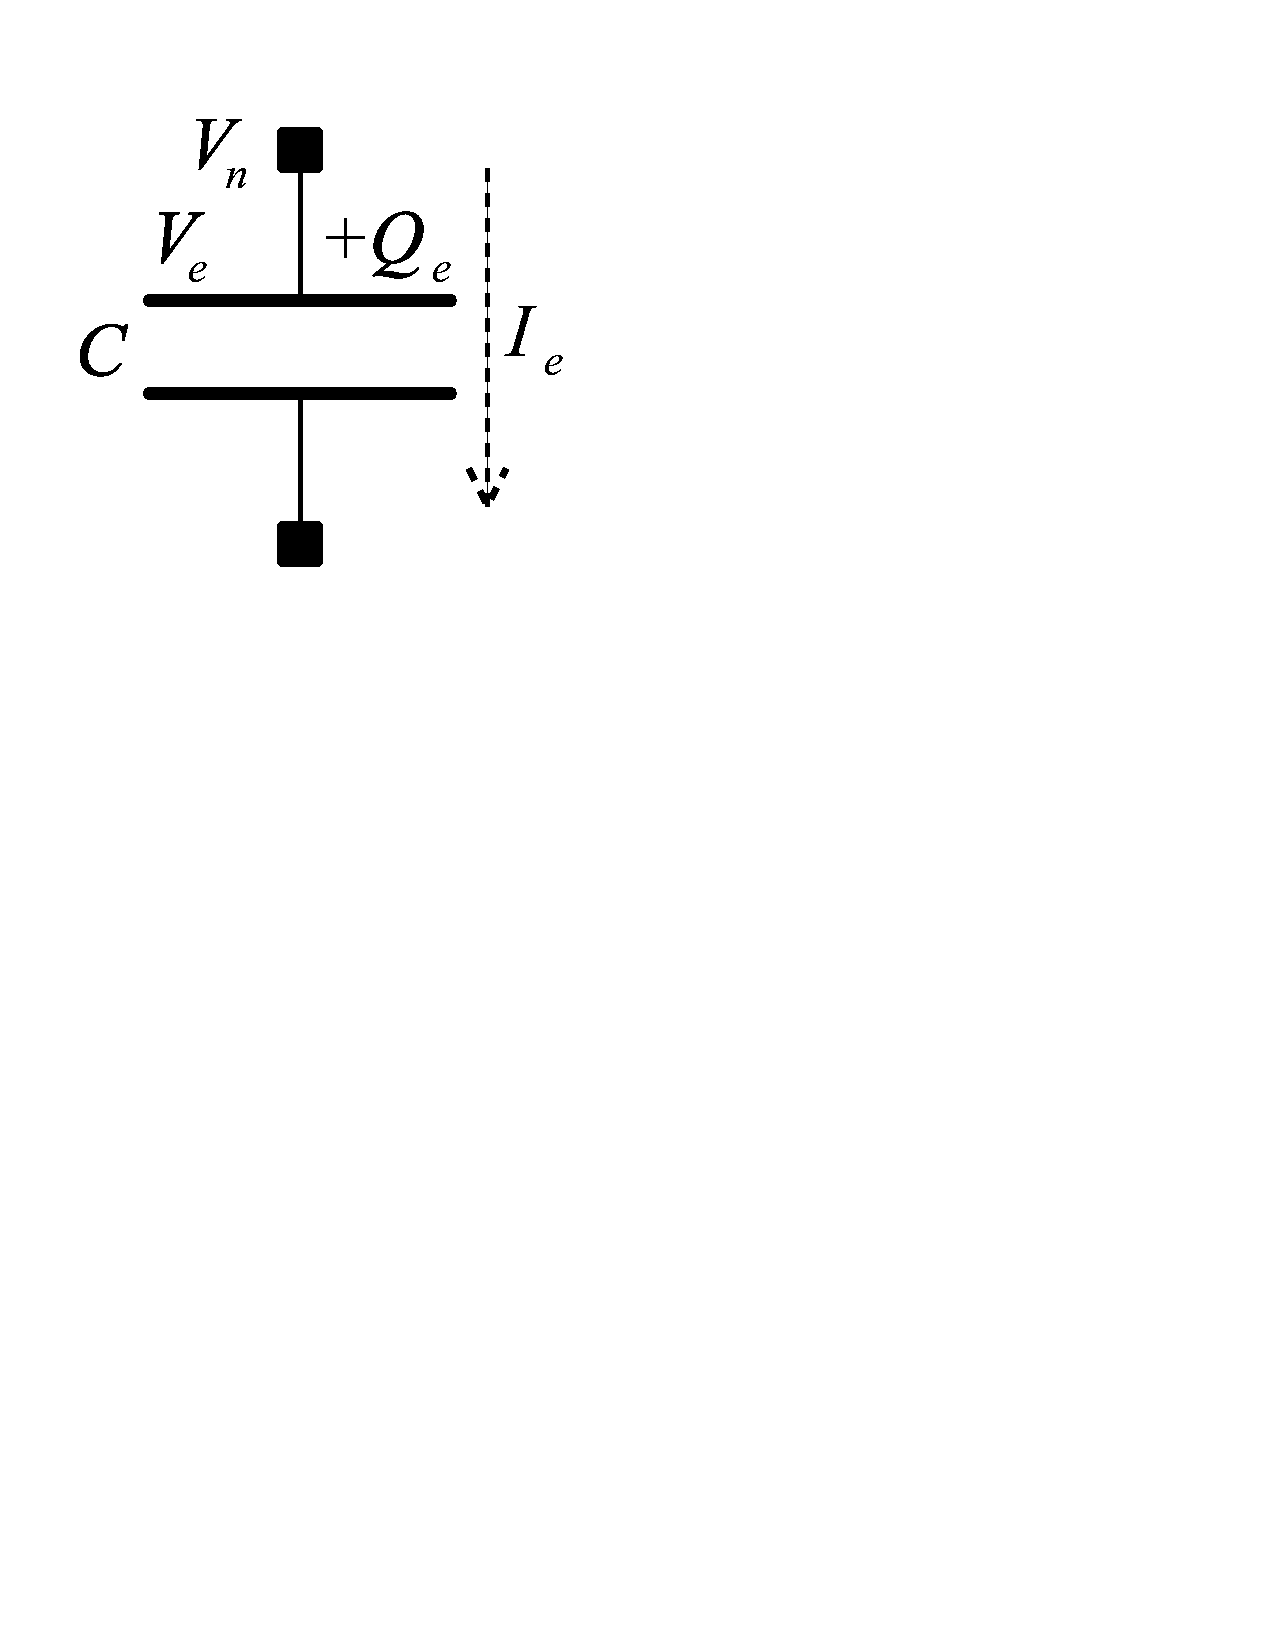
\includegraphics[trim = 0in 7in 4.5in 0in, clip, height=2in]{fig/electrode.pdf}
  \caption{Electrode element}
  \label{fig:Electrode_Element}
\end{figure}
The equation governing this element is,
\begin{eqnarray}
Q_e &=& C_e V_e
\end{eqnarray}
The matrix representation becomes,
\begin{eqnarray}
\left[
\begin{array}{ccc}
0 & 0 & \mathtt{lt}  \\
0 & 0 & 0  \\
0 & 0 & 0  \\
\end{array}
\right]
\left[
\begin{array}{c}
\dot{V}_n \\
\dot{V}_e \\
\dot{Q}_e
\end{array}
\right]
+
\left[
\begin{array}{rrr}
0  &  0 & 0  \\
0  &  0 &-1  \\
1  & -1 & 0
\end{array}
\right]
\left[
\begin{array}{c}
{V}_n \\
{V}_e \\
{Q}_e
\end{array}
\right]
=
\left[
\begin{array}{c}
0 \\
0 \\
0
\end{array}
\right]
\end{eqnarray}
$V_n$ represents the voltage variable at the node which
is linked to the finite element mesh. Two element variables
are introduced, $V_e$ and $Q_e$. 
$V_e$, which is additionally a global variable, is introduced 
to tie the selected
potentials of the finite element mesh to one variable. 
This global variable is then linked to $V_n$. Thus a 
shape function for the global variable must  be specified
for the formulation. $Q_e$ represents the total charge on 
the plate. 

The classes provides the following constructors:
\begin{codelist}

  \item[Electrode(vglobalid)] Creates an Electrode element 
  with \ttt{vglobalid}.

  \item[Electrode2(vglobalid)] Creates an Electrode element 
  with \ttt{vglobalid}.

\end{codelist}


\newpage
\section{Linear material models}
The set of linear models in Voigt notation can be expressed by the following
equation,
\begin{eqnarray}
\beps   &=& \bbD_{\bfE,T}\bsig + \bfd_{\bsig,T}   \bfE + \balpha_{\bsig,\bfE}\Delta T \\
\bfD    &=& \bfd_{\bfE,T}\bsig + \bkappa_{\bsig,T}\bfE + \bfp_{\bsig}\Delta T \\
\Delta S&=& \balpha_{\bfE,T}   + \bfp_{\bsig,T}   \bfE + \frac{C_{\bsig,\bfE}}{T}\Delta T
\end{eqnarray}
or in matrix notation,
\begin{eqnarray}
\left[
\begin{array}{c}
\beps  \\
\bfD   \\
\Delta S
\end{array}
\right]
&=&
\left[
\begin{array}{ccc}
\bbD_{\bfE,T}       & \bfd_{\bsig,T}     & \balpha_{\bsig,\bfE}    \\
\bfd_{\bfE,T}^T    & \bkappa_{\bsig,T}   & \bfp_{\bsig,\bfE}       \\
\balpha_{\bfE,T}^T & \bfp_{\bsig,T}^T    & \frac{C_{\bsig,\bfE}}{T}
\end{array}
\right]
\left[
\begin{array}{c}
\bsig \\
\bfE \\
\Delta T
\end{array}
\right]
\end{eqnarray}
Here,
$\beps$ denotes the linearized strain tensor, $\bsig$ the stress tensor, 
$\bfD$  the electric displacement, $\bfE$ the electric field,
$\Delta S$ the change in entropy, and $\Delta T$ the change in temperature.
The material dependent coeficients are denoted by,
$\bfs$ the compliance tensor, $\bfd$ the piezoelectric strain coeficient,
$\balpha$ the linear thermal expansion coeficient, 
$\bkappa$ the dielectric coeficient, $\bfp$ the pyroelectric coeficient,
$C$ the heat capacity, and $T$ is the reference temperature. The subscripts 
denote the fields which are taken
as constant in evaluating the coeficients.
We assume these coficients are represented in Voigt notation shown 
in Table \ref{table:VoigtNotation}
\begin{table}[htbp]
\caption{Voigt notation}
\label{table:VoigtNotation}
\begin{center}
\begin{tabular}{|c|cccccc|}
\hline
Voigt    &  1    &  2    &  3    &  4    &   5    &  6   \\
\hline
$(i,j)$  & (1,1) & (2,2) & (3,3) & (1,2) &  (2,3) & (3,1)\\
\hline
\end{tabular}
\end{center}
\end{table}
Additionally, the strain tensor in vector form is represented by,
\begin{eqnarray}
\beps &=& \left[ \beps_{11}, \beps_{22}, \beps_{33}, 2\beps_{12}, 2\beps_{23}, 2\beps_{31} \right]^T
\end{eqnarray}

Depending on the fields that are coupled, certain portions of the relation
above are extracted. Often, instead of the compliance $\bbD$, the inverse 
value representing the stiffness $\bbC=\bbD^{-1}$ is used. The number of 
material constants required to represent the material differ depending on
the geometry. 
These are summarized in Table \ref{table:CrystalDependentMaterialConstants}.

\begin{table}[htbp]
\centering
\caption{Material constants for different crystals}
\label{table:CrystalDependentMaterialConstants}
\begin{tabular}{|c||c|c|c|c|c|}
\hline
Crystal & Elastic($\bbC$) & Piezo($\bfd$) & Thermal($\balpha$) & Dielectric($\bkappa$) & Pyro($\bfp$) \\
\hhline{|=||=|=|=|=|=|}
Isotropic & $\bbC_{12}$,$\bbC_{44}$ & (-)   & $\balpha_T$     & $\bkappa$           & (-)          \\
\hline
Cubic     & $\bbC_{11}$,$\bbC_{12}$,$\bbC{44}$ & (-)& $\balpha_T$         & $\bkappa$             & (-)          \\
\hline
Hexagonal & $\bbC_{11}$,$\bbC_{12}$,$\bbC_{13}$,$\bbC_{33}$,$\bbC_{55}$ & $\bfd_{16}$,$\bfd_{31}$,$\bfd_{33}$
                                          & $\balpha_{T1}$,$\balpha_{T2}$ 
                                                               & $\bkappa_1$,$\bkappa_2$& (-)         \\
\hline
\end{tabular}
\end{table}

\clearpage
\subsection{Elasticity }
For elasticity, only the terms relatin stress and strain are 
extracted. The compliance tensor is inverted to obtain stress in
terms of strain as,
\begin{eqnarray}
\bsig = \bbC\beps \\
\bbC  = \bbD^{-1}
\end{eqnarray} 
The number of elastic constants that must be specified differ 
depending on the symmetry of the crystal.

\subsubsection{Isotropic material}
\begin{flushleft}
  \textbf{Required parameters in \ttt{mtype}:}
  [\ttt{E} and \ttt{nu}] or [\ttt{lambda} and \ttt{mu}]
\end{flushleft}

Two numbers define the elastic properties of an isotropic material.
In matrix form the stiffness is,
\begin{eqnarray}
\bbC_\text{isotropic} &=&
\left[
\begin{array}{cccccc}
\bbC_{12}+2\bbC_{44}  & \bbC_{12}  &  \bbC_{12}  &   0   &   0    &  0    \\
\bbC_{12}  & \bbC_{12}+2\bbC_{44} &  \bbC_{12}  &   0   &   0    &  0    \\
\bbC_{12}  & \bbC_{12}  &  \bbC_{12}+2\bbC_{44} &   0   &   0    &  0    \\
    0   &     0   &      0   & \bbC_{44} & 0 & 0 \\
    0   &     0   &      0   &   0   & \bbC_{44} &  0    \\
    0   &     0   &      0   &   0   &   0    & \bbC_{44}
\end{array}
\right] 
\end{eqnarray}
The values $\bbC_{12}$ and $\bbC_{44r}$ correspond to the Lame
constants $\lambda$ and $\mu$ and are related to the Youngs modulus
$E$ and Poisson ratio $\nu$ by,
\begin{eqnarray}
\bbC_{12} &=& \lambda = \frac{\nu E}{(1-2\nu)(1+\nu)} \\
\bbC_{44} &=& \mu     = \frac{E}{2(1+\nu)}
\end{eqnarray}
We can express the material tensors in a coordinate free notation
where given crystal
axes orientation $[\bfa,\bfb,\bfc]$, the elasticity tensor can be
expressed as,
\begin{eqnarray}
\bbC_{cubic} &=&  \bbC_{12}\rkTwoI\otimes\rkTwoI
                +2\bbC_{44}\rkFourIsym  \nonumber
\end{eqnarray}

\subsubsection{Cubic material}
\begin{flushleft}
  \textbf{Required parameters in \ttt{mtype}:}
  [\ttt{alpha}, \ttt{lambda}, and \ttt{mu}]
\end{flushleft}

Two numbers define the elastic properties of an isotropic material.
In matrix form the stiffness is,
\begin{eqnarray}
\bbC_\text{cubic} &=&
\left[
\begin{array}{cccccc}
\bbC_{11}  & \bbC_{12}  &  \bbC_{12}  &   0   &   0    &  0    \\
\bbC_{12}  & \bbC_{11}  &  \bbC_{12}  &   0   &   0    &  0    \\
\bbC_{12}  & \bbC_{12}  &  \bbC_{11}  &   0   &   0    &  0    \\
    0   &     0   &      0   & \bbC_{44} & 0 & 0 \\
    0   &     0   &      0   &   0   & \bbC_{44} &  0    \\
    0   &     0   &      0   &   0   &   0    & \bbC_{44}
\end{array}
\right]
\end{eqnarray}
The cubic coefficients are related to the usual expression for cubic
materials $\lambda, \mu, \alpha$ by the relations,
\begin{eqnarray}
\bbC_{11} &=& \alpha  \nonumber \\
\bbC_{12} &=& \lambda \nonumber \\
\bbC_{44} &=& \mu     \nonumber
\end{eqnarray}

We can express the material tensors in a coordinate free notation
where given
the cubic coeffecients $c_{11},c_{12},c_{c44}$ and crystal
axes orientation $[\bfa,\bfb,\bfc]$, the elasticity tensor can be
expressed as,
\begin{eqnarray}
\bbC_{cubic} &=&  c_{12}\rkTwoI\otimes\rkTwoI
                +2c_{44}\rkFourIsym
                + \left( c_{11}-c_{12}-2c_{44} \right)
                  \left(   \bfa \otimes \bfa \otimes \bfa \otimes \bfa
                         + \bfb \otimes \bfb \otimes \bfb \otimes \bfb
                         + \bfc \otimes \bfc \otimes \bfc \otimes \bfc \right)
                                                  \nonumber
\end{eqnarray}

\subsubsection{Hexagonal material}
\begin{flushleft}
  \textbf{Required parameters in \ttt{mtype}:}
  [\ttt{c11}, \ttt{c12}, \ttt{c13}, \ttt{c33}, and \ttt{c55}]
\end{flushleft}

The crystal has an in plane hexagonal structure giving
it an isotropic property in plane. The material begin piezoelectric
has no center of symmetry(inversion center). A hexagonal
crystal has the following structure for the elasticity tensor
$bbC_{hex}$, piezoelectric strain coefficients $\bfd_{hex}$ and
dielectric constants $\bkappa_{d\bsig}$ in Voigt notation.
The 1,2 axes are assumed to be in the isotropic crystal
plane with the 3 axis perpendicular to this plane.


\begin{eqnarray}
\bbC_{hex} &=&
\left[
\begin{array}{cccccc}
c_{11}  & c_{12}  &  c_{13}  &   0   &   0    &  0    \\
c_{12}  & c_{11}  &  c_{13}  &   0   &   0    &  0    \\
c_{13}  & c_{13}  &  c_{33}  &   0   &   0    &  0    \\
    0   &     0   &      0   & \frac{c_{11}-c_{12}}{2} & 0 & 0 \\
    0   &     0   &      0   &   0   & c_{55} &  0    \\
    0   &     0   &      0   &   0   &   0    & c_{55}
\end{array}
\right] 
\end{eqnarray}

In a hexagonal material, given the stiffness coefficients,
$c_{11},c_{12},c_{13},c_{33},c_{55}$, the elasticity tensor can
be expressed as,
\begin{eqnarray}
\bbC_{hex}  &=&                   c_{12}        \rkTwoI\otimes\rkTwoI
                + \left( c_{11} - c_{12} \right)\rkFourIsym
                                                    \nonumber\\
            & & + \left( c_{33} - c_{11} \right)
                  \left(   \bfc \otimes \bfc \otimes \bfc \otimes \bfc \right)
                                                    \nonumber\\
            & & + \left( c_{13} - c_{12} \right)
                  \left(   \bfa \otimes \bfa \otimes \bfc \otimes \bfc
                         + \bfc \otimes \bfc \otimes \bfa \otimes \bfa
                         + \bfb \otimes \bfb \otimes \bfc \otimes \bfc
                         + \bfc \otimes \bfc \otimes \bfb \otimes \bfb \right)
                                                     \nonumber\\
            & & + \left( c_{55} - \frac{c_{11}-c_{12}}{2} \right)
                  \left(   \bfb \otimes \bfc \otimes \bfb \otimes \bfc
                         + \bfb \otimes \bfc \otimes \bfc \otimes \bfb
                         + \bfc \otimes \bfb \otimes \bfb \otimes \bfc
                         + \bfc \otimes \bfb \otimes \bfc \otimes \bfb \right)
                                                     \nonumber\\
            & & + \left( c_{55} - \frac{c_{11}-c_{12}}{2} \right)
                  \left(   \bfc \otimes \bfa \otimes \bfc \otimes \bfa
                         + \bfc \otimes \bfa \otimes \bfa \otimes \bfc
                         + \bfa \otimes \bfc \otimes \bfc \otimes \bfa
                         + \bfa \otimes \bfc \otimes \bfa \otimes \bfc \right)
                                                     \nonumber
\end{eqnarray}


\clearpage
\subsection{Thermoelasticity }
For thermoelasticity, the terms relating stress,strain,entropy and temperature are
extracted. The compliance tensor is inverted to obtain stress in
terms of strain as,
\begin{eqnarray}
\left[
\begin{array}{c}
\bsig \\
\Delta S 
\end{array}
\right]
&=&
\left[
\begin{array}{cc}
\bbC & -\bbC\balpha \\
\balpha^T\bbC & \frac{C}{T}-\balpha^T\bbC\balpha
\end{array}
\right]
\left[
\begin{array}{c}
\beps \\
\Delta T
\end{array}
\right]
\end{eqnarray}
Additional to this, a constitutive equation must be given
for the heat flux $\bfq$. Standard linear Fourier model is assumed.
\begin{eqnarray}
\bfq = \bkappa_T\bfnabla T
\end{eqnarray}
where, $\bkappa_T$ is the conductivity tensor.

\subsubsection{Isotropic material}
\begin{flushleft}
  \textbf{Required parameters in \ttt{mtype}:}
  Parameters for isotropic elastic material plus [\ttt{at},\ttt{cp}, and \ttt{kt}]
\end{flushleft}
The elasticity tensor takes the form,
\begin{eqnarray}
\bbC &=& \bbC_\text{isotropic}
\end{eqnarray}
The linear thermal coeficient vector becomes,
\begin{eqnarray}
\balpha_T &=& \left[\balpha_T,\balpha_T,\balpha_T,0,0,0  \right]^T
\end{eqnarray}
The conductivity takes the form,
\begin{eqnarray}
\bkappa_T &=&
\left[
\begin{array}{ccc}
\bkappa_T & 0 & 0 \\
0 & \bkappa_T & 0 \\
0 & 0 & \bkappa_T
\end{array}
\right]
\end{eqnarray}

Two numbers define the elastic properties of an isotropic material.
In matrix form the stiffness is,

\subsubsection{Cubic material}
\begin{flushleft}
  \textbf{Required parameters in \ttt{mtype}:}
  Parameters for cubic elastic material plus [\ttt{at},\ttt{cp}, and \ttt{kt}]
\end{flushleft}
The elasticity tensor takes the form,
\begin{eqnarray}
\bbC &=& \bbC_\text{cubic}
\end{eqnarray}
The linear thermal coeficient vector becomes,
\begin{eqnarray}
\balpha_T &=& \left[\balpha_T,\balpha_T,\balpha_T,0,0,0  \right]^T
\end{eqnarray}
The conductivity takes the form,
\begin{eqnarray}
\bkappa_T &=&
\left[
\begin{array}{ccc}
\bkappa_T & 0 & 0 \\
0 & \bkappa_T & 0 \\
0 & 0 & \bkappa_T
\end{array}
\right]
\end{eqnarray}


\clearpage
\subsection{Piezoelectric elasticity }
For piezoelectric elasticity, the terms relating stress,strain,electric displacement and
electric field are
extracted. The compliance tensor is inverted to obtain stress in
terms of strain as,
\begin{eqnarray}
\left[
\begin{array}{c}
\bsig \\
\bfD
\end{array}
\right]
&=&
\left[
\begin{array}{cc}
\bbC & -\bbC\bfd \\
\bfd^T\bbC & \bkappa_{\bsig,T}-\bfd^T\bbC\bfd
\end{array}
\right]
\left[
\begin{array}{c}
\beps \\
\bfE
\end{array}
\right]
\end{eqnarray}

\subsubsection{Hexagonal material}
\begin{flushleft}
  \textbf{Required parameters in \ttt{mtype}:}
  Parameters for hexagonal elastic material plus [\ttt{kds1},\ttt{kds3},\ttt{d16},\ttt{d33} and \ttt{d31}]
\end{flushleft}
The elasticity tensor takes the form,
\begin{eqnarray}
\bbC &=& \bbC_\text{hexagonal}
\end{eqnarray}
The linear piezoelectric coeficient matrix becomes,
\begin{eqnarray}
\bfd &=& 
\left[
\begin{array}{cccccc}
0 & 0 & 0 & 0 & 0         & \bfd_{16} \\
0 & 0 & 0 & 0 & \bfd_{16} & 0         \\
\bfd_{31} & \bfd_{31} & \bfd_{33} & 0 & 0 & 0         
\end{array}
\right]
\end{eqnarray}
The permitivity takes the form,
\begin{eqnarray}
\bkappa_T &=&
\left[
\begin{array}{ccc}
\bkappa_1 & 0 & 0 \\
0 & \bkappa_1 & 0 \\
0 & 0 & \bkappa_3
\end{array}
\right]
\end{eqnarray}


\clearpage
\subsection{Electrostatics }
For an electrostatic problem, the terms relating electric displacement and
electric field are
extracted. 
\begin{eqnarray}
\bfD
&=&
\bkappa_{\bsig,T}
\bfE
\end{eqnarray}

\subsubsection{Isotropic material}
\begin{flushleft}
  \textbf{Required parameters in \ttt{mtype}:}
  Parameters for isotropic elastic material plus [\ttt{at},\ttt{cp}, and \ttt{kt}]
\end{flushleft}
The permitivity takes the form,
\begin{eqnarray}
\bkappa &=&
\left[
\begin{array}{ccc}
\bkappa & 0 & 0 \\
0 & \bkappa & 0 \\
0 & 0 & \bkappa
\end{array}
\right]
\end{eqnarray}

\clearpage
\subsection{Supporting functions}
\begin{codelist}
  \item[get\_material(mtype)] 
    Converts a material name \ttt{mtype} to a table of material
    properties and returns this table.
  \item[wafer\_orientation(wafer,angle)]
    Computes crystal axes for a cubic material given the wafer orientation
    \ttt{wafer}, either \ttt{'100'} or \ttt{'111'}, and the angle [rad]
    between 
    the global coordinate x-axis and a projection of a material axis 
    onto the x-y plane. A
    table \ttt{axis} containing the two 3-dimensional vectors which 
    define the direction of the x-y axes of the crystal will be returned,
    components of the axis1 followed by those of axis2. 
    \begin{figure}[htbp]
    \centering
    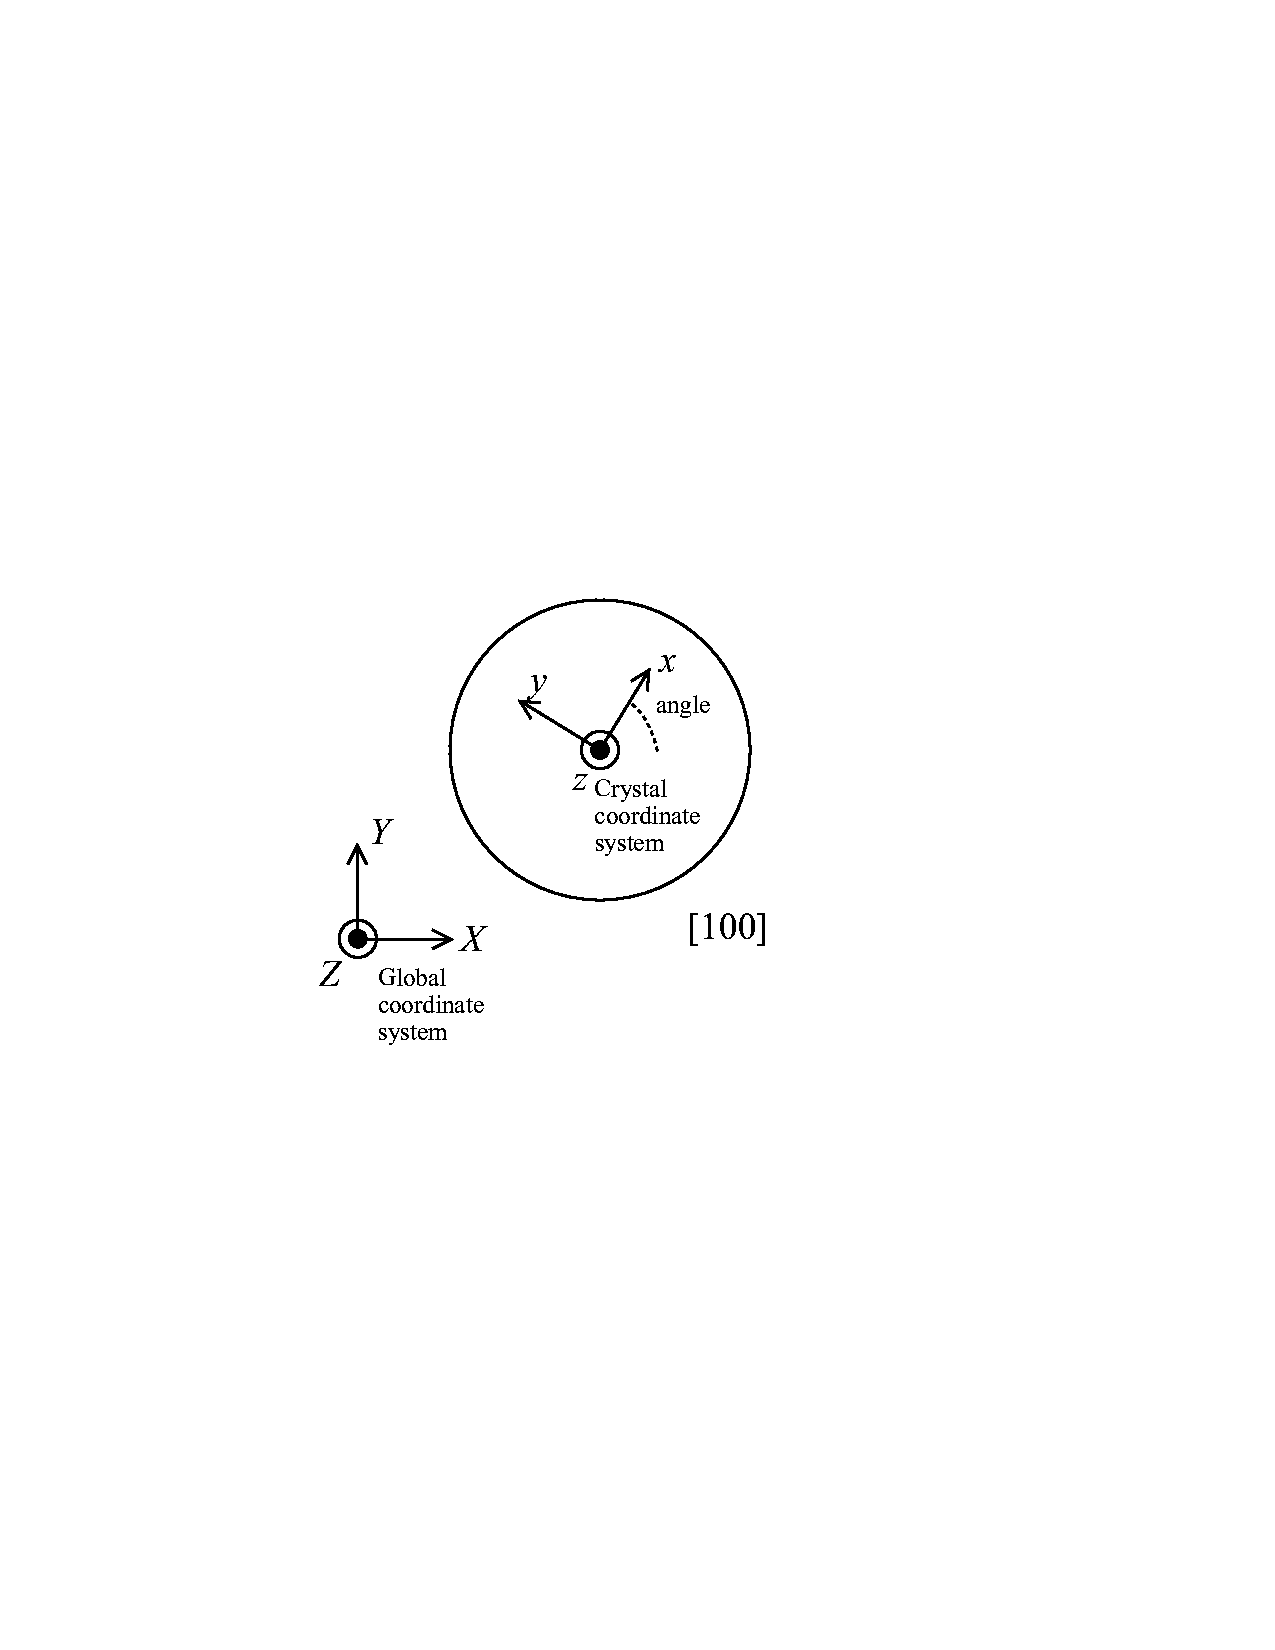
\includegraphics[trim=1.2in 4.0in 3.2in 3.0in, clip, height=2in]{fig/crystalaxis100.pdf}
    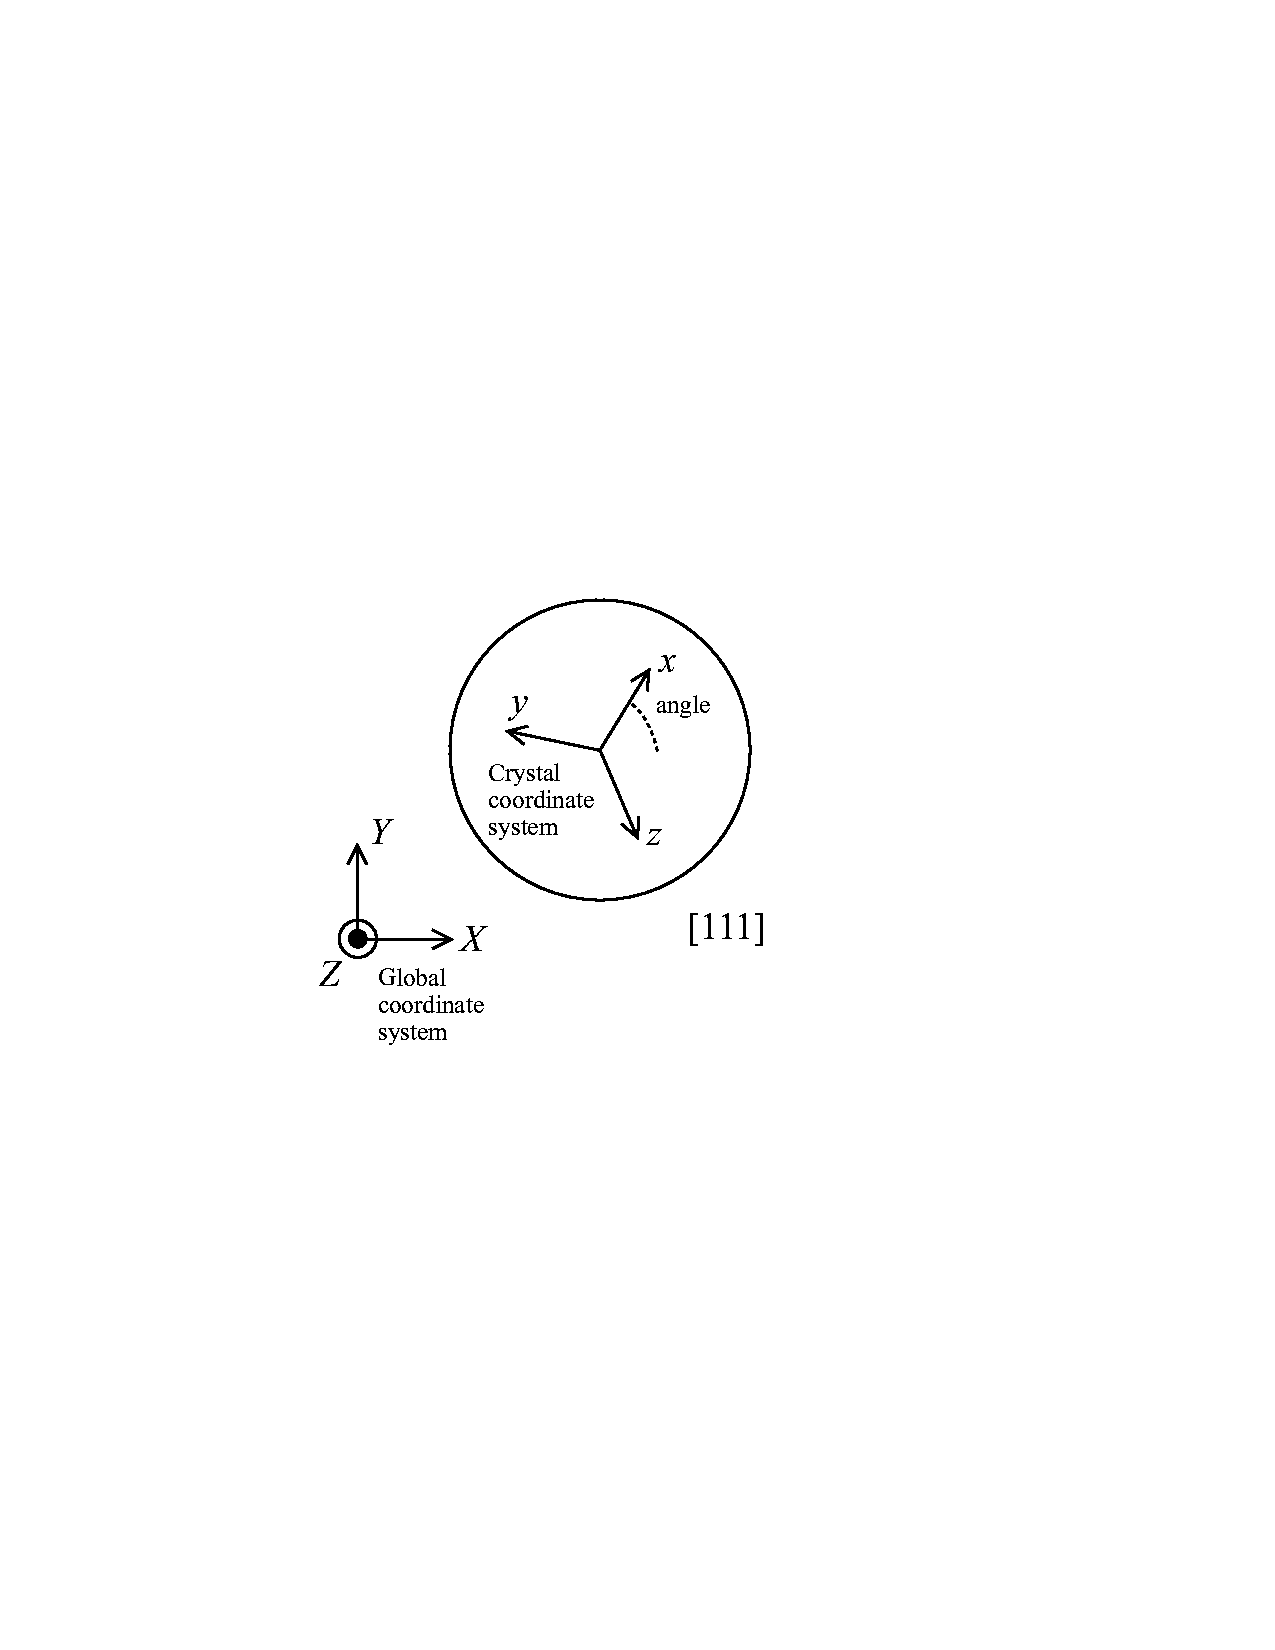
\includegraphics[trim=1.2in 4.0in 3.2in 3.0in, clip, height=2in]{fig/crystalaxis111.pdf}
    \caption{Crystal orientation (wafer and angle)}
    \label{fig:CrystalOrientation}
    \end{figure}
\end{codelist}

\begin{verbatim}
function isotropic_elasticity(mtype, etype, D)
function cubic_elasticity(mtype, etype, axis1, axis2, D)
function hexagonal_elasticity(mtype, etype, axis1, axis2, D)
\end{verbatim}
\begin{verbatim}
function isotropic_thermoelasticity(mtype, etype, Db)
function cubic_thermoelasticity(mtype, etype, axis1, axis2, Db)
\end{verbatim}
\begin{verbatim}
function piezoelectric_elasticity(mtype, etype, axis1, axis2, Db)
\end{verbatim}

\clearpage
\section{Non-dimensionalization}
The solution to involving coupled fields can
cause computational difficulties to the various
physical time scales that existent. As a result
the magnitude of the entries in the matrices can
vary tremendously, leading to very ill-conditioned
matrices. To circumvent this problem, non-dimensionalization
of dimensional parameters is conducted. 

\subsection{Incorporating non-dimensionalization}
Non-dimensionalization can easily be incorporated in the
analysis by specifying the functions summarized in 
Table~\ref{table:FunctionsNonDimensionalConstants}
at the beginning of the input file immediately
after the mesh construction. The only thing that the
user must take care is on which functions return 
dimensionalized values and which do not. Generally,
values which are intermediate results are returned in
non-dimensionlized form and those that are the final
results are dimensionalized. For instance, an array
returning just the free degrees of freedom would be 
non-dimensionalized as opposed to an array of nodal 
degrees of freedom at every node in the mesh would be 
dimensionalized.  
These are summarized in Tables 
\ref{table:DimensionalizingFunctions} and
\ref{table:NondimensionalizingFunctions}.
Thus if values are extracted from the arrays \ttt{disp}
or \ttt{force} obtained from,
\begin{verbatim}
      disp = Mesh_get_disp(mesh);
      force= Mesh_get_force(mesh);
\end{verbatim}
they will be in their dimensional form. Also extraction
of desired quantaties by multiplying \ttt{disp} or \ttt{force}
with the sense vectors obtained from,
\begin{verbatim}
      sense_disp_vec = Mesh_get_sense_disp(mesh,'disp_func');
      sense_force_vec= Mesh_get_sense_force(mesh,'force_func');
\end{verbatim}
will also result in dimensional results.

Vectors \ttt{U} or \ttt{F} obtained through,
\begin{verbatim}
      U = Mesh_get_u(mesh);
      F = Mesh_assemble_k(mesh) * U;
\end{verbatim}
will contain only the free dofs in their nondimensional form.
But multiplication of these vectors with the sense vectors
obtained through,
\begin{verbatim}
      sense_u_vec = Mesh_get_sense_u(mesh,'u_func');
      sense_f_vec = Mesh_get_sense_f(mesh,'f_func');
\end{verbatim}
will give dimensional results. 

See example of a MEMS cantilever in the Examples manual for
details on how to use these functions. 

\begin{table}[htbp]
\caption{Functions to evaluate non-dimensional constants}
\label{table:FunctionsNonDimensionalConstants}
\vspace{0.1in}
\centering
\begin{tabular}{l|m{2in}|l|l}
\hline
\multicolumn{1}{c|}{\tbf{Function name}} & 
\multicolumn{1}{c|}{\tbf{Required fields}}&
\multicolumn{1}{c|}{\tbf{Key constants}} & 
\multicolumn{1}{c}{\tbf{Aux constants}} \\
\hline
\hline
\ttt{mech\_nondim(mtype,cL)} &
\ttt{mtype.E}, \ttt{mtype.nu}, \ttt{mtype.rho}, \ttt{cL} &
\ttt{M,L,T} &
\ttt{F} \\
\hline
\ttt{ted\_nondim(mtype,cL)} &
\ttt{mtype.E},  \ttt{mtype.nu}, \ttt{mtype.rho}, 
\ttt{mtype.at}, \ttt{mtype.cp}, \ttt{mtype.kt}, 
(\ttt{mtype.T0} or \ttt{dim\_scales.T0}), \ttt{cL} &
\ttt{M,L,T,Th} &
\ttt{F,Qt} \\
\hline
\ttt{pz\_nondim(mtype,cL)} & 
\ttt{mtype.E},  \ttt{mtype.nu}, \ttt{mtype.rho}, 
\ttt{mtype.kds}, \ttt{mtype.d}, \ttt{cL} &
\ttt{M,L,T,A} &
\ttt{F,V,Q,E,R} \\
\hline
\ttt{em\_nondim(mtype,cL,(eps))} &
\ttt{mtype.E},  \ttt{mtype.nu}, \ttt{mtype.rho}, 
\ttt{mtype.kds}, \ttt{mtype.d}, \ttt{cL}, 
(\ttt{eps} or \ttt{mtype.eps} or \ttt{dim\_scales.eps})&
\ttt{M,L,T,A} &
\ttt{F,V,Q,E,R} \\
\hline
\end{tabular}
\end{table}

\begin{table}[htbp]
\centering
\caption{Returns dimensional quantaties}
\label{table:DimensionalizingFunctions}
\begin{tabular}{|l|m{3in}|}
\hline
function name & value returned \\
\hhline{|=|=|}
\ttt{Mesh\_x.m}                &  A coordinate of a specific node \\
\ttt{Mesh\_get\_x.m}           &  Array of nodal coordinates      \\
\hline
\ttt{Mesh\_get\_disp.m}        &  Array of nodal displacements    \\
\ttt{Mesh\_get\_force.m}       &  Array of nodal forces           \\
\hline
\ttt{Mesh\_get\_sense\_disp.m} &  Sense vector for nodal displacements \\
\ttt{Mesh\_get\_sense\_force.m}&  Sense vector for nodal forces        \\
\hline
\end{tabular}
\end{table}
\begin{table}[htbp]
\centering
\caption{Returns non-dimensional quantaties}
\label{table:NondimensionalizingFunctions}
\begin{tabular}{|l|m{3in}|}
\hline
function name & value returned \\
\hhline{|=|=|}
\ttt{Mesh\_get\_u.m}           & Vector of displacement free dofs       \\
\ttt{Mesh\_set\_u.m}           & Set a vector of displacement free dofs \\
\hline
\ttt{Mesh\_assemble\_k.m}            &Assemble stiffness matrix \\
\ttt{Mesh\_assemble\_mk.m}           &Assemble mass and stiffnes  matrices \\
\ttt{Mesh\_assemble\_mkc.m}          &Assemble mass,stiffness, and damping matrices \\
\ttt{Mesh\_assemble\_dR.m}           &Assemble gradient of residual \\
\ttt{Mesh\_assemble\_R.m}            &Assemble residual\\
\hline
\ttt{Mesh\_get\_sense\_u.m}    & Sense vector for displacement free dofs\\
\ttt{Mesh\_get\_sense\_f.m}    & Sense vector for force free dofs       \\
\ttt{Mesh\_get\_drive\_f.m}    & Drive vector for force free dofs       \\
\ttt{Mesh\_get\_sense\_globals\_u.m} &Sense vector for displacement global variable free dofs\\
\ttt{Mesh\_get\_sense\_globals\_f.m} &Sense vector for force global variable free dofs \\
\ttt{Mesh\_get\_sense\_globals\_f.m} &Sense vector for force global variable free dofs \\
\ttt{Mesh\_get\_drive\_elements\_u.m}&Drive vector for displacement element variable free dofs\\
\ttt{Mesh\_get\_sense\_elements\_f.m}&Sense vector for force global variable free dofs \\
\ttt{Mesh\_get\_drive\_elements\_f.m}&Drive vector for force global variable free dofs \\
\hline
\end{tabular}
\end{table}


\clearpage
\subsection{Compute non-dimensionalizing constants}

Depending on the fields that are involved, there are 
currently four functions shown in 
Table~\ref{table:FunctionsNonDimensionalConstants}
which compute the non-dimensionalizing
constants given representative material parameters and geometry.
The key constants are, \ttt{M}(mass), \ttt{L}(length),
\ttt{T}(time), \ttt{A}(current), and \ttt{Th}(temperature),
which are essential in non-dimensionalizing the appropriate fields.
The auxiliary constants, \ttt{F}(force), \ttt{Qt}(thermal flux),
\ttt{V}(voltage), \ttt{Q}(charge), \ttt{E}(e-field), and
\ttt{R}(resistance), are derived from these key constants.
Their dimensions are presented in 
Table~\ref{table:DimensionsOfAuxiliaryVariables}.

\begin{table}[htbp]
\caption{Dimensions of auxiliary variables}
\label{table:DimensionsOfAuxiliaryVariables}
\vspace{0.1in}
\centering
\begin{tabular}{c|l|c|c|c|c|c}
\hline
\multicolumn{1}{c|}{\tbf{Variable name}} &
\multicolumn{1}{c|}{\tbf{Field name}} &
\ttt{M} & \ttt{L} & \ttt{T} & \ttt{Th} & \ttt{A} \\ 
\hline
\hline
\ttt{F} & force        &  1 &  1 & -2 & - & - \\
\hline
\ttt{Qt}& thermal flux &  1 &  - & -3 & - & - \\
\hline
\ttt{Q} & current      &  - &  - &  1 & - & 1 \\
\ttt{V} & voltage      &  1 &  2 & -3 & - &-1 \\
\ttt{E} & e-field      &  1 &  1 & -3 & - &-1 \\
\ttt{R} & resistance   &  1 &  2 & -3 & - &-2 \\
\hline
\end{tabular}
\end{table}

Further details on how these are computed from the material 
properties are presented below in the codelist.
\begin{codelist}
  \item[mech\_nondim(mtype,cL)]
    Computes characteristic scales (\ttt{M,L,T}) and dimensional 
    quantaties (\ttt{F}) from a 
    table of material properties \ttt{mtype} and characteristic length
    scale \ttt{cL}, which are used for non-dimensionalization in a 
    mechanical problem. \ttt{mtype} must have the fields 
    \ttt{rho}(mass density) and \ttt{E} (Youngs modulus).
    \begin{eqnarray}
      \text{M} &=& \text{rho} * \text{cL}^3 \nonumber \\ 
      \text{L} &=& \text{cL}                \nonumber \\
      \text{T} &=& \frac{\text{cL}}{\sqrt{\text{E/rho}}} \nonumber 
    \end{eqnarray}
    A table named \ttt{dim\_scales} with these fields is returned. 
  \item[ted\_nondim(mtype,cL)] 
    Computes characteristic scales (\ttt{M,L,T,Th}) and dimensional 
    quantaties (\ttt{F,Qt}) from a 
    table of material properties \ttt{mtype} and characteristic length
    scale \ttt{cL}, which are used for non-dimensionalization in a 
    mechanical problem. \ttt{mtype} must have the fields 
    \ttt{rho}(mass density) and \ttt{E} (Youngs modulus),
    \ttt{at}(linear coefficient of thermal expansion), 
    \ttt{cp}(specific heat at constant pressure),
    and \ttt{T0}(ambient temperature).
    \begin{eqnarray}
      \text{M} &=& \text{rho} * \text{cL}^3 \nonumber \\ 
      \text{L} &=& \text{cL}                \nonumber \\
      \text{T} &=& \frac{\text{cL}}{\sqrt{\text{E/rho}}} \nonumber \\
      \text{Th}&=& \frac{\text{T0 * at * E}}{\text{rho*cp}} \nonumber
    \end{eqnarray}
    A table named \ttt{dim\_scales} with these fields is returned.
  \item[pz\_nondim(mtype,cL)] 
    Computes characteristic scales (\ttt{M,L,T,A}) and dimensional 
    quantaties (\ttt{F,V,Q,E,R}) from a 
    table of material properties \ttt{mtype} and characteristic length
    scale \ttt{cL}, which are used for non-dimensionalization in a 
    piezoelectric mechanical problem. \ttt{mtype} must have the fields 
    \ttt{rho}(mass density) and \ttt{E} (Youngs modulus),
    \ttt{kds}(permitivity at constant stress), 
    and \ttt{d}(piezoelectric strain coefficients).
    \begin{eqnarray}
      \text{M} &=& \text{rho} * \text{cL}^3 \nonumber \\ 
      \text{L} &=& \text{cL}                \nonumber \\
      \text{T} &=& \frac{\text{cL}}{\sqrt{\text{E/rho}}} \nonumber \\
      \text{A} &=& \frac{\text{kds * cL}^2}{\text{d * T}} \nonumber 
    \end{eqnarray}
    A table named \ttt{dim\_scales} with these fields is returned.
  \item[em\_nondim(mtype,cL,(eps))] 
    Computes characteristic scales (\ttt{M,L,T,A}) and dimensional 
    quantaties (\ttt{F,V,Q,E,R}) from a 
    table of material properties \ttt{mtype} and characteristic length
    scale \ttt{cL}, which are used for non-dimensionalization in a 
    electromechanical problem. \ttt{mtype} must have the fields 
    \ttt{rho}(mass density) and \ttt{E} (Youngs modulus),
    and \ttt{eps}(permitivity at constant stress).
    \begin{eqnarray}
      \text{M} &=& \text{rho} * \text{cL}^3 \nonumber \\ 
      \text{L} &=& \text{cL}                \nonumber \\
      \text{T} &=& \frac{\text{cL}}{\sqrt{\text{E/rho}}} \nonumber \\
      \text{A} &=& \frac{\text{eps * E * cL}^3}{\text{T}} \nonumber
    \end{eqnarray}
\end{codelist}

\subsection{Non-dimensionalize material parameters}
\begin{codelist}
  \item[material\_normalize(ftype,...)]
    Non-dimensionalizes all arguments \ttt{...} by the the dimensional
    scale \ttt{dim\_scales[ftype]}. \ttt{ftype} must be a string corresponding
    to a characteristic scale (\ttt{M,L,T,Th,A}) or a dimensional quantaty
    \ttt{F,V,Q,E,R,Qt,etc.} that has been predefined in the table 
    \ttt{dim\_scales}. If such a field does not exist, 
    \ttt{dim\_scales[ftype]} is assumed one. The number of input arguments
    will be returned.
  \item[mech\_material\_normalize(m)]
    Non-dimensionalizes the mechanical fields of the material \ttt{m} 
    given as a table by the characteristic scales defined in \ttt{dim\_scales}, 
    and returns a table with ONLY these mechanical fields. There is no 
    restriction on the fields existing in \ttt{m}, but only the fields,
    \ttt{rho, E, lambda, mu, alpha, c11, c12, c13, c33, c55} will be 
    non-dimensionalized. 
    If a field in \ttt{dim\_scales} does not exist, it
    will be assumed one. 
  \item[ted\_material\_normalize(m)]
    Non-dimensionalizes the thermomechanical fields of the material \ttt{m} 
    given as a table by the characteristic scales defined in \ttt{dim\_scales}, 
    and returns a table with ONLY these thermomechanical fields. There is no 
    restriction on the fields existing in \ttt{m}, but only the fields,
    \ttt{rho, E, lambda, mu, alpha, at, cp, kt, T0} will be 
    non-dimensionalized.
    If a field in \ttt{dim\_scales} does not exist, it
    will be assumed one. 
  \item[pz\_material\_normalize(m)]
    Non-dimensionalizes the piezoelectric-mechanical fields of the 
    material \ttt{m} 
    given as a table by the characteristic scales defined in \ttt{dim\_scales}, 
    and returns a table with ONLY these piezoelectric-mechanical fields. 
    There is no 
    restriction on the fields existing in \ttt{m}, but only the fields,
    \ttt{rho, c11, c12, c13, c33, c55, d16, d31, d33, kds1, kds3} will be 
    non-dimensionalized.
    If a field in \ttt{dim\_scales} does not exist, it
    will be assumed one. 
\end{codelist}

\newpage
\section{Basic functions (Matlab)}

\subsection{Loading and deleting Lua mesh input files}
The Lua object interface is used in the MATLAB \ttt{Mesh\_load}
function:
\begin{codelist}

  \item[Mesh\_load(filename,p)]
    Creates a Lua interpreter and executes the named file in order to
    generate a mesh object (which is returned).  The mesh should be
    named ``mesh''; if such an object is undefined on output,
    \ttt{Mesh\_load} returns an error message.  Before executing
    the named file, \ttt{Mesh\_load} copies the entries of the
    structure \ttt{p}, which may only be strings or doubles, into
    the Lua global state; in this way, it is possible to vary mesh
    parameters from MATLAB.

  \item[Mesh\_delete(mesh)]
    Deletes the mesh object.

\end{codelist}

\subsection{Getting Scaling parameters}
\begin{codelist}

  \item[scale\_param = Mesh\_get\_scale(scale\_name)]
  Get a characteristic scale described by the given name.

  \item[{[cu,cf]} = Mesh\_get\_scales(mesh)]
  Return an array of dimensional scales for the problem.
\begin{verbatim}
  Outputs:
   cu - scales for the primary variables
   cf - scales for the secondary (flux) variables
\end{verbatim}

\end{codelist}

\subsection{Obtain basic information about mesh}
\begin{codelist}

  \item[ndm = Mesh\_get\_ndm(mesh)]
  Return the dimension of the ambient space for the mesh.

  \item[numnp = Mesh\_numnp(mesh)]
  Return the number of nodal points in the mesh.

  \item[ndf = Mesh\_get\_ndf(mesh)]
  Return the number of degrees of freedom per node in the mesh.

  \item[numid = Mesh\_get\_numid(mesh)]
  Return the total number of degrees of freedom in the mesh.

  \item[numelt = Mesh\_numelt(mesh)]
  Return the number of elements in the mesh.

  \item[nen = Mesh\_get\_nen(mesh)]
  Return the maximum number of nodes per element.

  \item[numglobals = Mesh\_numglobals(mesh)]
  Return the number of global degrees of freedom in the mesh

  \item[nbranch\_id = Mesh\_nbranch\_id(mesh)]
  Return the number of branch variables in the mesh

  \item[x = Mesh\_get\_x(mesh, (cL))]
  Return an ndm-by-numnp array of node positions.
\begin{verbatim}
  Inputs:
  cL - characteristic length used for redimensionalization
        (default: mesh 'L' scale)
\end{verbatim}

  \item[e = Mesh\_get\_e(mesh)]
  Return the element connectivity array (a maxnen-by-numelt array).

  \item[id = Mesh\_get\_id(mesh)]
  Return the variable-to-identifier mapping (a maxndf-by-numnp array).
  Nodal variables subject to displacement BCs are represented by a 0.

  \item[bc = Mesh\_get\_bc(mesh)]
  Return an ndf-by-numnp array of boundary codes.  The codes are
\begin{verbatim}
  0 - No boundary condition for this dof
  1 - Displacement (essential) boundary conditions
  2 - Flux (natural) boundary conditions
\end{verbatim}

  \item[{[p,e,id,bc,numnp]} = Mesh\_get\_parameters(mesh,(cL))]
\begin{verbatim}
  Input:
  cL    - characteristic length to redim node positions
          (default: mesh 'L' parameter)
  Return mesh parameters:
  p     - Node position array
  e     - Element connectivity array (nen-by-numelt)
  id    - Variable identifier array (ndf-by-numnp)
  bc    - Boundary condition codes (see Mesh\_get\_bc)
  numnp - Number of nodal points
\end{verbatim}

\end{codelist}

\subsection{Obtain particular information about ids}
\begin{codelist}

  \item[ix = Mesh\_ix(mesh,i,j)]
  Return the ith node of element j

  \item[id = Mesh\_id(mesh,i,j)]
  Return the ith variable of node j

  \item[id = Mesh\_branchid(mesh,i,j)]
  Return the ith variable of branch j

  \item[id = Mesh\_globalid(mesh,j)]
  Return the id for jth global variable

  \item[nbranch\_id = Mesh\_nbranch\_id(mesh,j)]
  Return the number of variables of branch j

\end{codelist}

\subsection{Obtain particular information about id, nodes, or elements}
\begin{codelist}

  \item[x = Mesh\_x(mesh,i,j,(cL))]
  Return the ith coordinate of node j.
\begin{verbatim}
  Inputs:
   i  - coordinate index
   j  - node number
   cL - characteristic length scale for redimensionalization
        (default: mesh 'L' scale)
\end{verbatim}

  \item[nen = Mesh\_get\_nen\_elt(mesh,j)]
  Return the number of nodes for element j

\end{codelist}

\subsection{Getting displacements and force}
\begin{codelist}

  \item[{[u]} = Mesh\_get\_disp(mesh,is\_dim)]
  Get the node displacement array (dimensionless)
\begin{verbatim}
  Inputs:
   - is\_dim - should the vector be redimensionalized? (default: 1)
\end{verbatim}

  \item[{[f]} = Mesh\_get\_force(mesh,is\_dim)]
  Get the node force array (dimensionless)
\begin{verbatim}
  Inputs:
   - is\_dim - should the vector be redimensionalized? (default: 1)
\end{verbatim}

  \item[{[u]} = Mesh\_get\_u(mesh, cx, cv, ca, reduced, is\_dim)]
  Get the node displacement array (dimensionless)
\begin{verbatim}
  Inputs:
   - cx  For variables (default: 1)
   - cv  For 1st derivative variables
   - ca  For 2nd derivative variables
   - reduced or not?
\end{verbatim}

  \item[Mesh\_set\_u(mesh, u, v, a)]
  Set the displacement, velocity, and acceleration vectors.
  The vectors should be in dimensionless form.
\begin{verbatim}
  Inputs:
   u - displacement vector (or zero or no arg to clear the mesh u)
   v - velocity vector     (or zero or no arg to clear the mesh v)
   a - acceleration vector (or zero or no arg to clear the mesh a)
\end{verbatim}

\end{codelist}


\subsection{Functions to form global matrices}
\begin{codelist}

  \item[{[K]} = Mesh\_assemble\_k(mesh)]
  Assemble the stiffness matrix for the mesh.
  Matrix is in dimensionless form.

  \item[{[M,K]} = Mesh\_assemble\_mk(mesh)]
  Assemble the mass and stiffness matrices for the mesh.
  Matrices are in dimensionless form.

  \item[{[M,K,C]} = Mesh\_assemble\_mkc(mesh)]
  Assemble the mass, stiffness, and damping matrices.
  Matrices are in dimensionless form.

  \item[{[K]} = Mesh\_assemble\_dR(mesh, cx, cv, ca, reduced)]
  Assembles mass, damping, or stiffness matrix from mesh.
\begin{verbatim}
  If 'reduced' is given     -'reduced=1' Reduced form
                           -'reduced=0' Non-reduced form
\end{verbatim}
  Matrices are in dimensionless form.

  \item[[K] = Mesh\_element\_dR(mesh, eltid, cx, cv, ca)]
  Gets scattered mass, damping, or stiffness matrix from mesh element.
  Matrices are in dimensionless form.

  \item[{[R,Ri] = Mesh\_assemble\_R(mesh)}]
  Assemble the system residual vector and return it in R and Ri.
  The residual vector is in dimensionless form.
\begin{verbatim}
  Outputs:
    R  - real part of the residual vector
    Ri - imag part of the residual vector
\end{verbatim}

\end{codelist}

\subsection{Other useful functions}
\begin{codelist}
  \item[ E = Mesh\_mean\_power(mesh)]
  Compute the time-averaged energy flux at each node.
  TODO: The flux is currently in dimensionless form, but it probably
   shouldn't be.

  \item[f = Mesh\_get\_lua\_fields(mesh, name, nfields)]
  Return an array of field values.
\begin{verbatim}
  Inputs:
   name      - the name of the Lua function to define the fields
   nfields   - number of fields requested
\end{verbatim}

  \item[Mesh\_make\_harmonic(mesh,omega)]
  Set v = i*omega*u and a = -omega**2*u
\begin{verbatim}
  Input:
   omega - forcing frequency
   units - specify units of forcing frequency (default 'rs'):
     'hz': omega is in units of Hz
     'rs': omega is in units of rad/s
     'nd': omega is in dimensionless units
      cT : nondimensionalize omega using the given characteristic time
\end{verbatim}

\end{codelist}

\subsection{Assigning and reassigning ids}
\begin{codelist}
  \item[int = Mesh\_assign\_ids(mesh)]
  Number the degrees of freedom in the mesh.
  Returns the total number of dofs.

  \item[int = ted\_block\_mesh(mesh)]
  Relabel the nodal degrees of freedom so that all mechanical degrees of
  freedom come first, followed by all thermal degrees of freedom.  Return
  the total number of mechanical degrees of freedom.

  \item[int = pz\_block\_mesh(mesh)]
  Relabel the nodal degrees of freedom so that all mechanical degrees of
  freedom come first, followed by all potential degrees of freedom.  Return
  the total number of mechanical degrees of freedom.

\end{codelist}

\subsection{Producing forcing and sensing pattern vectors}
\begin{codelist}

  \item[u = Mesh\_get\_sense\_u(mesh, name, is\_reduced)]
  Return a vector for a displacement sense pattern.
  The vector is in dimensionless form.
\begin{verbatim}
  Inputs:
    name       - the name of the Lua function to define the pattern
   is\_reduced - do we want the reduced (vs full) vector?  Default: 1
\end{verbatim}

  \item[u = Mesh\_get\_sense\_disp(mesh, name, is\_reduced)]
  Return a vector for a displacement sense pattern.
  The vector is in dimension form.
\begin{verbatim}
  Inputs:
   name       - the name of the Lua function to define the pattern
   is\_reduced - do we want the reduced (vs full) vector?  Default: 1
\end{verbatim}

  \item[f = Mesh\_get\_sense\_f(mesh, name, is\_reduced)]
  Return a vector for a force sense pattern
  The vector is in dimensionless form.
\begin{verbatim}
  Inputs:
   name       - the name of the Lua function to define the pattern
   is\_reduced - do we want the reduced (vs full) vector?  Default: 1
\end{verbatim}

  \item[f = Mesh\_get\_drive\_f(mesh, name, is\_reduced)]
  Return a vector for a drive sense pattern
  The vector is in dimensionless form.
\begin{verbatim}
  Inputs:
   name       - the name of the Lua function to define the pattern
   is\_reduced - do we want the reduced (vs full) vector?  Default: 1
\end{verbatim}

  \item[f = Mesh\_get\_sense\_force(mesh, name, is\_reduced)]
  Return a vector for a force sense pattern
  The vector is in dimension form.
\begin{verbatim}
  Inputs:
   name       - the name of the Lua function to define the pattern
   is\_reduced - do we want the reduced (vs full) vector?  Default: 1
\end{verbatim}

  \item[u = Mesh\_get\_sense\_globals\_u(mesh, name)]
  Return a vector for a global variable displacement sense pattern.
  The vector is in dimensionless form.
\begin{verbatim}
  Inputs:
    name       - the name of the Lua function to define the pattern
\end{verbatim}

  \item[f = Mesh\_get\_sense\_globals\_f(mesh, name)]
  Return a vector for a global variable force sense pattern.
  The vector is in dimensionless form.
\begin{verbatim}
  Inputs:
    name       - the name of the Lua function to define the pattern
\end{verbatim}

  \item[f = Mesh\_get\_drive\_globals\_f(mesh, name)]
  Return a vector for a global variable force drive pattern.
  The vector is in dimensionless form.
\begin{verbatim}
  Inputs:
    name       - the name of the Lua function to define the pattern
\end{verbatim}

  \item[u = Mesh\_get\_sense\_elements\_u(mesh, name)]
  Return a vector for an element variable displacement sense pattern.
  The vector is in dimensionless form.
\begin{verbatim}
  Inputs:
    name       - the name of the Lua function to define the pattern
\end{verbatim}

  \item[f = Mesh\_get\_sense\_elements\_f(mesh, name)]
  Return a vector for an element variable force sense pattern.
  The vector is in dimensionless form.
\begin{verbatim}
  Inputs:
    name       - the name of the Lua function to define the pattern
\end{verbatim}

  \item[f = Mesh\_get\_drive\_elements\_f(mesh, name)]
  Return a vector for an element variable force drive pattern.
  The vector is in dimensionless form.
\begin{verbatim}
  Inputs:
    name       - the name of the Lua function to define the pattern
\end{verbatim}

\end{codelist}

\subsection{Getting and setting variables in the Lua environment}
\begin{codelist}

  \item[Lua\_set\_string(L, string\_name, string\_value)]
  Set a string variable in the Lua environment
\begin{verbatim}
  L            - the Lua interpreter object
  string\_name - the name of the Lua variable(must be string)
  s    - a string value(must be string)
\end{verbatim}

  \item[string = Lua\_get\_string(L, string\_name)]
  Get a string variable out of the Lua environment
\begin{verbatim}
  L    - the Lua interpreter object.
  name - the name of the Lua variable.
\end{verbatim}
  Returns an empty string if no such variable exists.

  \item[Lua\_set\_double(L, double\_name, double\_value)]
  Set a numeric variable in the Lua environment
\begin{verbatim}
  L    - the Lua interpreter object
  name - the name of the Lua variable
  x    - a number
\end{verbatim}

  \item[{[x]} = Lua\_get\_double(L, name)]
  Get a numeric variable out of the Lua environment
\begin{verbatim}
  x  - the value of the Lua variable   
\end{verbatim}

  \item[Lua\_set\_table\_double(L, table\_name, double\_name, double\_value x)]
  Set a numeric variable in a table in the Lua environment
\begin{verbatim}
  L     - the Lua interpreter object
  table\_name  - the name of the Lua table
  double\_name - the name of the Lua key
  double\_value- a number
\end{verbatim}
  key can be a number or a string.

  \item[{[x]} = Lua\_get\_table\_double(L, table\_name, double\_name)]
  Get a numeric variable out of a table in the Lua environment
\begin{verbatim}
  x  - the value of the Lua variable   
\end{verbatim}
  key can be a number or a string.

  \item[Lua\_set\_table\_string(L, table\_name, string\_name, string\_value)]
  Set a string variable in a table in the Lua environment
\begin{verbatim}
  L     - the Lua interpreter object
  table\_name  - the name of the Lua table
  string\_name - the name of the Lua key
  string\_value- a number
\end{verbatim}
  key can be a number or a string.

  \item[{[s]} = Lua\_get\_table\_string(L, table\_name, string\_name)]
  Get a string variable out of a table in the Lua environment
\begin{verbatim}
  s  - the string value of the Lua variable   
\end{verbatim}
  key can be a number or a string.

  \item[Lua\_set\_array(L, aname, array, a\_type)]
  Set a matrix variable in the Lua environment
\begin{verbatim}
  Input:
   L        - the Lua interpreter object
   aname    - the name of the matrix variable
   array    - a numeric array
   a\_type(0)- the type of array to construct
             0: Real array
             1: Real array of twice the size
                 (Not supported yet)
             2: Complex array
\end{verbatim}

  \item[{[m\_Object]} = Lua\_get\_array(L, name)]
  Get a matrix variable from the Lua environment
\begin{verbatim}
  Input:
  L     - the Lua interpreter object
  name  - the name of the Lua variable
\end{verbatim}

\end{codelist}

\subsection{Manipulating the Lua environment}
The same interfaces that are automatically bound to Lua are also
automatically bound to MATLAB.  In addition, several methods are
defined which allow MATLAB to manipulate a Lua interpreter:
\begin{codelist}

  \item[Lua\_open]      
    Return a pointer to a new Lua interpreter \ttt{L}

  \item[Lua\_close(L)]  
    Close the Lua interpreter

  \item[Lua\_dofile(L,filename)]
    Execute a Lua file

  \item[Lua\_set\_mesh(L,name,mesh)]
    Assign a mesh object to a Lua global

  \item[Lua\_get\_mesh(L,name)]
    Retrieve a mesh object from a Lua global

\end{codelist}

\clearpage
\section{Functions for analysis(MATLAB)}
\subsection{Static analysis}
  Solves for the static state of a device. The equation,
\begin{eqnarray}
  \bfR(\bfU) = 0
\end{eqnarray}
  for the general case, and 
\begin{eqnarray}
\bfK\bfU = \bfF
\end{eqnarray}
  for the linear case is solved. 

\begin{codelist}

  \item[static\_state(mesh,opt)]
  Solves for the static state. If the field nonlinear is 
  not specified only 1 iteration will be conducted.
\begin{verbatim}
 Input: mesh  - Mesh object
       *opt
         nonlinear('NR')- Conduct non-linear solve
                       'NR' :Newton-Raphson
                       'MNR':Modified-Newton-Raphson
         kmax(20)      - Max number of iterations
         du_tol(1e-15) - Tolerance for convergence
                         for increment
         R_tol (1e-15) - Tolerance for convergence
                         for residual
         U             - Initial starting vector for solve
\end{verbatim}

\end{codelist}

\subsection{Time-harmonic analysis}
Solves for the time harmonic state.
\begin{eqnarray}
\left(\bfK + i\omega \bfC - \omega^2\bfM\right)\bfu = \bfF
\end{eqnarray}

\begin{codelist}

 \item[harmonic\_state(mesh,F,w,opt)]
 Solves for the time-harmonic state.
\begin{verbatim}
 Input: mesh     - Mesh object
        F        - Forcing vector(in nondimensional form)
        w        - Forcing frequency
       *opt
         mkc(0)        - Include damping matrix
         kmax(1)       - Max number of iterations
         du_tol(1e-15) - Tolerance for convergence
                        for increment
         R_tol(1e-15)  - Tolerance for convergence
                        for residual
\end{verbatim}

\end{codelist}

\clearpage
\subsection{Modal analysis}
The MATLAB sparse eigensolver routine \ttt{eigs} is actually an
interface to ARPACK (see Section~\ref{section-eigs}).  We express all
frequencies in radians/s rather than Hertz.  We provide one function
to compute complex frequencies and associated mode shapes for PML
eigenvalue problems:
\begin{codelist}

  \item[{[V,w,Q]} = pml\_mode(M,K,w0,nmodes,opt)]
    Find the requested number of modes closest in frequency to
    \ttt{w0}.  Return an array of mode shapes, a vector of complex
    frequencies, and a vector of $Q$ values.  Options are 
    \begin{codelist}[use\_umfpack]
      \item[use\_matlab]  Use MATLAB's eigs rather than ARPACK?
      (default: false)
      \item[use\_umfpack]  Use UMFPACK with MATLAB eigs, if present?
      (default: true)
      \item[disp]  Verbosity level? (default: 0)
    \end{codelist}

   \item[{[V,w,Q]} = tedmode(mesh, w0, nev, opt)]
   Computes the eigenfrequencies and modes of a thermoelastic problem.
\begin{verbatim}

 Compute nev complex frequencies w (in rad/s) near target frequency
 w0, and also associated Q values.  V contains the eigenvectors
 (mechanical and thermal parts).

 *Note*: tedmode will reorder the degrees of freedom in the mesh.

 opt   contains optional parameters:
   mech - Conduct purely mechanical analysis
   type - Use a perturbation method ('pert') or linearization
          ('full').  Default is 'full'.
   T0   - Baseline temperature for use in symmetric linearization
   cT   - Characteristic time scale for redimensionalization
          (Default: Mesh_get_scale('T')
   use_matlab - use matlab eigs or not (Default:0)
\end{verbatim}

   \item[{[V,w,Q]} = emmode(mesh, w0, nev, opt)]
   Computes the eigenfrequencies and modes of a electromechanical problem.
\begin{verbatim}
 Compute nev complex frequencies w (in rad/s) near target frequency
 w0, and also associated Q values.  V contains the eigenvectors


 opt   contains optional parameters:
   mech - Conduct purely mechanical analysis
   type - Use a perturbation method ('pert') or linearization
          ('full').  Default is 'full'.
   cT   - Characteristic time scale for redimensionalization
          (Default: Mesh_get_scale('T')
   use_matlab - use matlab eigs or not (Default:1)
   idg_m - array of global numbers for mechanical variables
   idg_p - array of global numbers for potential variables

\end{verbatim}

   \item[{[V,w,Q]} = emcmode(mesh, w0, nev, opt)]
   Computes the eigenfrequencies and modes of a electromechanical problem with 
   surrounding circuitry.
\begin{verbatim}
 Compute nev complex frequencies w (in rad/s) near target frequency
 w0, and also associated Q values.  V contains the eigenvectors


 opt must contain following parameters
   eno - array of element numbers for electrodes
   idg - array of global number for driving electrode

 opt   contains optional parameters:
   mech - Conduct purely mechanical analysis
   type - Use a perturbation method ('pert') or linearization
          ('full').  Default is 'full'.
   cT   - Characteristic time scale for redimensionalization
          (Default: Mesh_get_scale('T')
   use_matlab - use matlab eigs or not (Default:1)

\end{verbatim}

\end{codelist}

\clearpage
\subsection{Transfer function evaluation}
\begin{codelist}

  \item[{[H,freq]} = second\_order\_bode(mesh,wc,drive\_pat,sense\_pat,opt)]
  Computes the transfer function given the driving pattern and sensing pattern.
  The frequency range is set by specifying the center frequency \ttt{wc} and
  the range. Model reduction can be conducted by specifying the number of iterations
  \ttt{kmax} conducted to produce the reduced order model. Different projection 
  bases can also be selected.
\begin{verbatim}

   Output: freq          - Frequency array [rad/s]
           H             - Output
   Input:  mesh          - the mesh input
           wc            - center frequency[rad/s]
           drive_pat     - Driving pattern vector
           sense_pat     - Sensing pattern vector
          *opt
          -freq          - Predefined array of freq
          -mkc(0)        - Include damping or not
          -cT            - Characteristic time scale for
                           redimensionalization
                           (Default: Mesh_get_scale('T')
          -wr_min(0.90)  - left  value mag of bode plot
          -wr_max(1.10)  - right value mag of bode plot
          -w_ndiv(50)    - number divisions in bode plot
          -w_type('lin') - division type (linspae or logspace)
          -kmax(0)       - number of arnoldi iterations
          -realbasis(0)  - use real basis??
          -structurep(0) - use structure preserving basis??
          -use_umfpack   - use UMFPACK?? (Default: use if exist)
 If kmax and wc are given, use model reduction via an Arnoldi
 expansion about the shift w0.  
\end{verbatim}

\end{codelist}

\subsection{Model reduction}
There is currently one model reduction routine in the MATLAB support
files for \hiq.  As before, all frequencies are expressed in radians/s
rather than Hz.
\begin{codelist}

  \item[{[Mk,Dk,Kk,Lk,Bk,Vk]} = rom\_arnoldi(M,K,l,b,kk,w0,opt)] 
    Takes \ttt{kk} steps of
    shift-and-invert Arnoldi to form a basis for the Krylov subspace
    $\mathcal{K}_k\left( (K-(2 \pi \omega_0)^2 M)^{-1} M, b \right)$
    in order to form a reduced system to estimate the system transfer
    function.  Returns reduced matrices $M_k$, $K_k$, $l_k$, and
    $b_k$, along with the projection basis $V_k$.  If
    \ttt{opt.realbasis} is set to true (default is false), then the
    projection will use a real basis for the span of $[\Re(V_k),
    \Im(V_k)]$.  To do this, the matrix $[\Re(V_k), \Im(V_k)]$ will be
    orthonormalized using an SVD, and vectors corresponding to values
    less than \ttt{opt.realtol} (default $10^{-8}$) will be dropped.

   \item[{[Mk,Dk,Kk,Lk,Bk,Vk]} = rom\_soar(M,D,K,L,B,kk,w0,opt)]
    Takes \ttt{kk} steps of 
    shift-and-invert SOAR to form a basis for the second order 
    Krylov subspace,
    in order to form a reduced system to estimate the system transfer
    function.  Returns reduced matrices $M_k$, $K_k$, $l_k$, and
    $b_k$, along with the projection basis $V_k$.  If
    \ttt{opt.realbasis} is set to true (default is false), then the
    projection will use a real basis for the span of $[\Re(V_k),
    \Im(V_k)]$.  To do this, the matrix $[\Re(V_k), \Im(V_k)]$ will be
    orthonormalized using an SVD, and vectors corresponding to values
    less than \ttt{opt.realtol} (default $10^{-8}$) will be dropped.
    To form the structure preserving base for the thermoelastic problem,
    the id array must be reordered so that the mechanical dofs come first
    before the thermal dofs. \ttt{opt.structurep} must be set to 1, and 
    the number of mechanical degrees of freedom must also be specified.

\end{codelist}

\newpage
\section{Basic analysis (Lua)}
\subsection{Functions to obtain basic information about mesh}
\begin{codelist}

  \item[ndm = Mesh:get\_ndm()]
  Return the dimension of the ambient space for the mesh.

  \item[numnp = Mesh:numnp()]
  Return the number of nodal points in the mesh.

  \item[ndf = Mesh:get\_ndf()]
  Return the number of degrees of freedom per node in the mesh.

  \item[numid = Mesh:get\_numid()]
  Return the total number of degrees of freedom in the mesh.

  \item[numelt = Mesh:numelt()]
  Return the number of elements in the mesh.

  \item[nen = Mesh:get\_nen()]
  Return the maximum number of nodes per element.

  \item[numglobals = Mesh:numglobals()]
  Return the number of global degrees of freedom in the mesh

  \item[nbranch\_id = Mesh:nbranch\_id()]
  Return the number of branch variables in the mesh

\end{codelist}

\subsection{Obtain particular information about ids}
\begin{codelist}

  \item[id = Mesh:id(mesh,i,j)]
  Return the ith variable of node j

  \item[id = Mesh:branchid(mesh,i,j)]
  Return the ith variable of branch j

  \item[id = Mesh:globalid(mesh,j)]
  Return the id for jth global variable

  \item[nbranch\_id = Mesh:nbranch\_id(mesh,j)]
  Return the number of variables of branch j

\end{codelist}





%\begin{verbatim}
%- plotmesh(mesh) to plot the mesh what boundary codes mean
%-- F =-Mesh_assemble_R(mesh);
%-- K = Mesh_assemble_k(mesh);
%%-- U = K\F;
%-- Mesh_set_u(mesh, U);
%-- disp = Mesh_get_disp(mesh);
%-- plotfield2d(mesh);
%-- Mesh_delete(mesh);
%-- Mesh_get_id(mesh);
%-- How do you compute stresses???
%\end{verbatim}
%\subsection{Static analysis}
%\subsection{Modal analysis}
%\subsection{Time-harmonic analysis}
%\subsection{Model reduction}

\newpage
\section{Plotting results (Matlab)}
\subsection{Mesh plots}
There are several plotting routines for viewing the behavior of 2D
meshes:
\begin{codelist}

  \item[plotmesh(mesh,opt)]  Plots a given mesh.  Options are
    \begin{codelist}
      \item[anchors]  Marker for nodes with displacement BC
        (default: \ttt{'g+'})
      \item[forces]   Marker for nodes with force BC
        (default: \ttt{'r+'})
      \item[deform]   Deform mesh according to first to fields of $u$?
        (default: false)
      \item[clf]      Clear the figure before display?
        (default: true)
      \item[axequal]  Use equal axes in plots? (default: false)
    \end{codelist}

\end{codelist}


\subsection{Plotting the deformed mesh}

\begin{codelist}

  \item[plotfield1d(mesh,opt)]
  Colors are chosen according to the magnitudes of the u components.
      \begin{codelist}
      \item[ufields]  Fields to use for displacement 
        (default: \ttt{[1]})
      \item[cfields]  Fields to use for coloring
        (default: \ttt{[1]})
      \item[ncfields] Number of color Fields to obtain
      \item[axequal]  Use equal axes in plots? (default: false)
      \item[subplot]  Subplot setup (default: \ttt{[length(nfields), 1]})
      \item[deform]   Deform mesh according to first to fields of $u$?
        (default: false)
      \item[clf]      Clear the figure before display?
        (default: true)
      \item[axis]     Set axes
      \item[subplot]  Subplot size (default is [nfields 1])
      \item[xscale]   Amount to scale by (for unit change)(Default:1)
      \item[xlabel]   X label (Default: [])
      \item[ylabel]   Y label (Default: []) 
      \item[titles]   Title (can be a cell array of titles)(Default: []) 
      \end{codelist}

  \item[plotfield2d(mesh,opt)]
  Colors are chosen according to the magnitudes of the u components.
      \begin{codelist}
      \item[ufields]  Fields to use for displacement 
        (default: \ttt{[1,2]})
      \item[cfields]  Fields to use for coloring
        (default: \ttt{[1,2]})
      \item[ncfields] Number of color Fields to obtain(defualt:1)
      \item[cbias]    Bias of the color scale (cmax/cbias->red)(default: 3)
      \item[cbar]     Add colorbar (Default: false)
      \item[cscale]   Scale field colors together? (Default: false)
      \item[axequal]  Use equal axes in plots? (default: false)
      \item[subplot]  Subplot setup (default: \ttt{[length(nfields), 1]})
      \item[deform]   Deform mesh according to first to fields of $u$?
        (default: false)
      \item[clf]      Clear the figure before display?
        (default: true)
      \item[axis]     Set axes
      \item[subplot]  Subplot size (default is [nfields 1])
      \item[xscale]   Amount to scale by (for unit change)(Default:1)
      \item[xlabel]   X label (Default: [])
      \item[ylabel]   Y label (Default: []) 
      \item[titles]   Title (can be a cell array of titles)(Default: []) 
      \end{codelist}

\end{codelist}

\subsection{Animations}

\begin{codelist}

  \item[plotcycle1d(mesh,s,opt)]
    Plot an animation of the motion of the mesh.  The amplitude of
    motion is scaled by the factor \ttt{s} (which defaults to one
    if it is not provided).  The frames can be written to disk as a
    sequence of PNG files to make a movie later.
    The following options can be set through the \ttt{opt} structure
    \begin{codelist}[framepng]
      \item[framepng] Format string for movie frame files (default: [])
      \item[nframes]  Number of frames to be plotted (default: 32)
      \item[fpcycle]  Frames per cycle (default: 16)
      \item[startf]   Start frame number (default: 1)
      \item[fpause]   Pause between re-plotting frames (default: 0.25)
      \item[axequal]  Use equal axes in plots? (default: false)
      \item[axis]     Set axes
      \item[subplot]  Subplot size (default is [nfields 1])
      \item[xscale]   Amount to scale by (for unit change)(Default:1)
      \item[xlabel]   X label (Default: [])
      \item[ylabel]   Y label (Default: []) 
      \item[titles]   Title (can be a cell array of titles)(Default: []) 
      \item[avi\_file]Title of avi file to generate(Default: []) 
                         (Default: NO AVI FILE IS PRODUCED)
      \item[avi\_w]    Width  of the window size(Default: 300) 
      \item[avi\_h]    Height of the window size(Default: 300) 
      \item[avi\_left] Window distance from left side of monitor(Default: 10) 
      \item[avi\_bottom]Window distance from bottom    of monitor(Default: def) 
                        (Default is set so window touches top of monitor)
    \end{codelist}


  \item[plotcycle2d(mesh,s,opt)]
    Plot an animation of the motion of the mesh.  The amplitude of
    motion is scaled by the factor \ttt{s} (which defaults to one
    if it is not provided).  The frames can be written to disk as a
    sequence of PNG files to make a movie later.
    The following options can be set through the \ttt{opt} structure
    \begin{codelist}[framepng]
      \item[framepng] Format string for movie frame files (default: [])
      \item[nframes]  Number of frames to be plotted (default: 32)
      \item[fpcycle]  Frames per cycle (default: 16)
      \item[startf]   Start frame number (default: 1)
      \item[fpause]   Pause between re-plotting frames (default: 0.25)
      \item[cscale]   Color all fields on the same scale? (default: false)
      \item[cbias]    Bias of the color scale (cmax/cbias->red)(default: 3)
      \item[ufields]  Fields to use for displacement 
        (default: \ttt{[1 2]})
      \item[cfields]  Fields to use for coloring
        (default: \ttt{[1 2]})
      \item[axequal]  Use equal axes in plots? (default: false)
      \item[subplot]  Subplot setup (default: \ttt{[length(cfields), 1]})

      \item[axis]     Set axes
      \item[subplot]  Subplot size (default is [nfields 1])
      \item[xscale]   Amount to scale by (for unit change)(Default:1)
      \item[xlabel]   X label (Default: [])
      \item[ylabel]   Y label (Default: []) 
      \item[titles]   Title (can be a cell array of titles)(Default: []) 
      \item[avi\_file]Title of avi file to generate(Default: []) 
                         (Default: NO AVI FILE IS PRODUCED)
      \item[avi\_w]    Width  of the window size(Default: 300) 
      \item[avi\_h]    Height of the window size(Default: 300) 
      \item[avi\_left] Window distance from left side of monitor(Default: 10) 
      \item[avi\_bottom]Window distance from bottom    of monitor(Default: def) 
                        (Default is set so window touches top of monitor)

    \end{codelist}
\end{codelist}

\subsection{Plotting Bode plots}

In addition, there is a function for viewing Bode plots:
\begin{codelist}

  \item[plot\_bode(freq,H,opt)]
    Plots a Bode plot.  \ttt{H} is the transfer function evaluated
    at frequency points \ttt{freq}.  The option structure \ttt{opt}
    may contain the following options:
    \begin{codelist}[magnitude]
    \item[usehz]     Assume \ttt{freq} is in Hz (default: false)
    \item[logf]      Use a log scale on the frequency axis (default: false)
    \item[magnitude] Plot magnitude only (default: false)
    \item[visualQ]   Visually compute $Q$ for the highest peak (default: false)
    \item[lstyle]    Set the line style for the plot (default: \ttt{'b'})
    \end{codelist}
    For example, to plot a reduced model Bode plot on top of an exact
    Bode plot, we might use the following code:
    \begin{verbatim}
  figure(1); hold on
  opt.logf = 1;
  opt.lstyle = 'b' ; plot_bode(freq_full, H_full, opt);
  opt.lstyle = 'r:'; plot_bode(freq_rom,  H_rom,  opt);
  hold off
    \end{verbatim}

\end{codelist}
It is also possible to simultaneously show a deformed mesh and a Bode
plot with a marker indicating the excitation frequency.
\begin{codelist}
  \item[plotmesh\_bode(mesh,f,H,fcurrent,opt)]
    Plot the deformed mesh and create a Bode plot.  The \ttt{opt}
    field is passed through to \ttt{plotmesh}.
\end{codelist}


\end{document}
